\documentclass[../PhD.tex]{subfiles}

\begin{document}

%%%%%%%%%%%%%%%%%%%%%%%%%%%%%%%%%%%%%%%%%
%%%%%%%%%%%%%%%%%%%%%%%%%%%%%%%%%%%%%%%%%

\chapter{Perturbative Stability of Massless Scalars in AdS$_4$}
\label{ch: ttf}

Having examined the collapse of massive scalars fields in AdS$_5$, we now wish to explore the perturbatively stable solutions for massless scalars. These solutions resist gravitational collapse and give analytic descriptions of the direct and inverse energy cascades that must be balanced for stability to be achieved. 

The Two-Time Formalism (TTF) allows for renormalization flow equations that absorb secular terms into renormalized integration constants in the first-order solution for the scalar field. These flow equations become algebraic under a quasi-periodic (QP) ansatz for the amplitudes and phases. While the TTF theory technically involves an infinite sum of terms, by truncating the series to a finite $\jm$ value, numerical values for the amplitudes and phases can be calculated. How the truncation value affects the space of solutions, and the limits of the solution space itself, remains to be addressed.

\section{Contributions of Authors}

In this collaboration, QP solutions to \eqref{qp eqn} were found numerically through programs initially written by N.~Deppe, but later expanded and developed by myself. In particular, I developed code to achieve the tail fitting and seeding procedure detailed in appendix~\ref{app: seeding} that allowed for solutions to \eqref{qp eqn} to be developed for $\jm$ values of several hundred -- almost an order of magnitude greater than the solutions previously found in the literature. Implementation of the high temperature perturbation method outlined in \ref{ssec: highT} was done using code I developed, as was the procedure of reoptimization that allowed for the high temperature solution to be projected back to the QP solution surface at various frequencies. Finally, I developed the constant-$T$ solution finding method using a Newton-Raphson solver. Evolution of the solutions was based on numerical methods initially developed by N.~Deppe, then further developed by me. All data management and analysis was done using programs I wrote.

Much of the numerical work for this project was done using the University of Winnipeg's tesla server, where CPU hours are not tracked. However, for larger systems increased computing power was required, which necessitated transferring all code to Compute Canada's new Cedar cluster. Once there, I used 5.43 CPU years' worth of computing power to run evolutions and analysis of the results. Finally, I have written the manuscript, with input from the other authors, that appears here.

As is common for these types of projects, all members of the collaboration were equally involved in the interpretation of the data, as well as the late stages of editing. Authors are listed alphabetically and it is understood that all members contribute equally to the publication.

\newpage

%%%%%%%%%%%%%%%%%%%%%%%%%%%%%%%%%%%%%%%%%
%%%%%%%%%%%%%%%%%%%%%%%%%%%%%%%%%%%%%%%%%

\begin{center}
{\bf{\Large On the Stability of High-Temperature, Quasi-Periodic Solutions for Massless Scalars in AdS$_4$}} \\
\bigskip
{\bf To Appear on \href{https://arxiv.org}{arxiv.org}} \\
\bigskip
\bigskip
Brad Cownden$^1$, Nils Deppe$^2$, and Andrew R.~Frey$^{1,3}$\\
\bigskip

$^1${\it Department of Physics \& Astronomy,\\ University of Manitoba\\
66 Chancellors Cir, Winnipeg, Manitoba R3T 2N2, Canada}
\vspace{0.1in}

$^2${\it Cornell Center for Astrophysics and Planetary Science and
Department of Physics,\\ Cornell University\\
122 Sciences Drive, Ithaca, New York 14853, USA}
\vspace{0.1in}

$^3${\it Department of Physics and Winnipeg Institute for Theoretical
Physics,\\ University of Winnipeg\\
515 Portage Avenue, Winnipeg, Manitoba R3B 2E9, Canada }
\end{center}

\bigskip

We examine a family of numerical solutions in the Two-Time Formalism (TTF) description of massless scalars in AdS$_4$ parameterized by the dimensionless parameter $T$. Numerical solutions can only be found by truncating a sum over frequency components to some finite number. However, any numerical solution must be robust against an increase in the number of frequencies. We extensively verify the robustness of such solutions against truncation, and over a range of $T$. We find that solutions with low values of $T$ are in general robust as the number of modes is increased, while solutions with higher values of $T$ are not. Finally, we examine the evolution of possible quasi-periodic solutions within the TTF description and show that low-$T$ solutions maintain their quasi-periodicity while higher $T$ solutions do not.

%%%%%%%%%%%%%%%%%%%%%%%%%%%%%%%%%%%%%%%%%
%%%%%%%%%%%%%%%%%%%%%%%%%%%%%%%%%%%%%%%%%

\section{Introduction}

The question of the nonperturbative stability of ($d+1$)-dimensional Anti-de Sitter spacetime against horizon formation has been examined extensively, both as a question of mathematical physics and given its application to the AdS/CFT correspondence; see reviews such as \cite{1708.05600}. Beginning with the seminal work of \cite{1104.3702}, others (including \cite{1108.4539, 1106.2339, 1110.5823, 1210.0890, 1510.02592}) have repeatedly demonstrated the generic instability of spherically symmetric AdS$_{d+1}$ gravity minimally coupled to a scalar field. The primary driver of the instability in the fully nonlinear system is the turbulent flow of energy to short length scales. However, \cite{1303.3186, 1307.2875, 1403.5434} and others have shown that some initial conditions in asymptotically AdS spacetimes resist gravitational collapse; these conditions form islands of stability in the space of initial data. As these islands of stability continue to be explored, more subtle behaviours continue to be identified, particularly along the ``shorelines'' \cite{1508.02709, 1711.00454,1602.03535, 1803.02830}. Within the stability islands are various solutions created from exciting a single linear mode, known as oscillons or breathers for real scalars \cite{1104.3702,1210.0890,1303.3186,1503.07746}, boson stars for complex scalars (on a fixed metric)\cite{1304.4166,1307.2875}, and geons in pure gravity \cite{1109.1825,1208.5772}.

While the nonperturbative physics of AdS instability requires numerical study, the perturbative formulation is purely analytical and encapsulates the weakly turbulent physics at $\mc O(\epsilon^3)$ in a small-amplitude expansion. The linear-order system is simply a massless scalar in global AdS whose solution is written as a sum over the spatial eigenfunctions of AdS. At this order, the scalar field is stable for all times. The next-to-leading order in the expansion -- $\mc O(\epsilon^3)$ for the scalar field -- gives an equation of motion for the scalar field that is sourced by the scalar's backreaction with non-trivial metric functions. It is at this order that resonant sources terms arise which grow with time and invalidate the perturbative description. When only a single eigenmode is excited, resonances can be removed by frequency shifts; however, multimode data contain resonances that cannot be removed this way \cite{1109.1825}. For fields constructed from multiple excited eigenmodes, the secular growth of resonant terms triggers the onset of instability \cite{1109.1825, 1306.0317, 1312.5544, 1506.03519}.

To describe the secular growth, the amplitude and phase of each eigenmode are allowed to flow with respect to time. Applying renormalization techniques to these new slowly-varying amplitudes and phases leads to a ladder of coupled first-order ordinary differential equations describing the flow.  There are several equivalent methods to arrive at the flow equations: the Two-Time Formalism (TTF) -- wherein the slow time $\tau = \epsilon^2 t$ is the flow parameter \cite{1403.6471} -- a renormalization-like formalism \cite{1407.6273,1412.3249}, and time averaging procedure \cite{1412.3249,1510.07836}. The $\mc O(\epsilon^3)$ resonances are then controlled by absorbing the secular terms into the renormalized amplitudes and phases.

In order to numerically solve the flow equations for a general scalar field, one naturally must truncate the mode expansion at a maximum eigenmode number $\jm$. By taking a quasi-periodic (QP) ansatz for the amplitude and phase variables, we are guaranteed a stable solution. These QP solutions, like all other solutions in the TTF description, have constant energy $E$ and particle number $N$, and families of solutions are parameterized by a unit-less ``temperature" parameter $T= E/N$ \cite{1403.6471,1507.08261}. Understanding the bounds of the space of QP solutions allows us to better understand how to construct more general long-lived scalar fields. QP solutions are special in that the time-dependence of each mode is harmonic, so QP solutions satisfy algebraic equations. The first family of low-temperature solutions is found by directly solving these algebraic equations. High temperature solutions were purportedly found by \cite{1507.08261} through repeatedly perturbing low-temperature solutions up to a maximum temperature of $T_{max} = 2\jm + d$. 

In this work, we ask when QP solutions to the truncated TTF theory extend to the full untruncated theory. We explore the space of high temperature solutions using established perturbative methods, and solutions are tested against various choices of $\jm$. We then examine the stability of both classes of solutions through indicators such as the scalar curvature and energy transfer among eigenmodes. 

This work is organized as follows: we begin in \S~\!\ref{sec: scalar in AdS} with a review of the linearized solutions for a minimally coupled, massless scalar field in AdS$_{d+1}$, as well as the renormalization flow equations that govern the time evolution of the amplitudes and phases in the TTF theory. In \S~\!\ref{sec: qp}, we find quasi-periodic solutions in AdS$_4$ by numerically solving a set of algebraic equations and establish the bounds of low-temperature QP solutions. We then consider methods of probing the space of QP solutions to include high-temperature solutions in \S\!~\ref{ssec: highT}, and examine the evolution of all QP solutions within the perturbative theory in \S\!~\ref{sec: time evolution}. We end with a discussion of results in \S~\!\ref{sec: ttf discussion}. 

%%%%%%%%%%%%%%%%%%%%%%%%%%%%%%%%%%%%%%%%%
%%%%%%%%%%%%%%%%%%%%%%%%%%%%%%%%%%%%%%%%%

\section{Minimally Coupled Scalar Fields in AdS$_{d+1}$}
\label{sec: scalar in AdS}

Consider a spherically-symmetric, asymptotically AdS$_{d+1}$ spacetime with characteristic curvature $L=1$. Written in Schwarzschild-like coordinates, the metric is given by
\begin{align}
ds^2 = \frac{1}{\cos^2(x)} \left( -Ae^{-2\delta} dt^2 + A^{-1}dx^2 + \sin^2(x) d\Omega^{d-1}\right) \, ,
\end{align}
where the radius $x \in [0,\pi/2]$ and $-\infty < t < \infty$. A minimally-coupled, massless scalar field $\phi(t,x)$ is subject to the following Einstein and Klein-Gordon equations:
\begin{align}
\label{EEs}
G_{ab} + \Lambda g_{ab} &= 8\pi \left( \nabla_a \phi \nabla_b \phi - \frac{1}{2} g_{ab} (\nabla \phi)^2 \right) \\
\label{KG}
0 &= \frac{1}{\sqrt{-g}} \p_a \sqrt{-g} \, g^{ab} \p_b \phi \, .
\end{align}
The canonical equations of motion for the scalar field are
\begin{align}
\p_t \phi = A e^{-\delta} \Pi, \quad \p_t \Phi = \p_x ( A e^{-\delta} \Pi), \quad \text{and} \quad \p_t \Pi = \frac{\p_x \left(\Phi A e^{-\delta} \tan^{d-1} (x) \right)}{\tan^{d-1}(x)} \, ,
\end{align}
where the canonical momentum is $\Pi(t,x) = A^{-1}e^\delta \phi$ and $\Phi(t,x) \equiv \p_x \phi$ is an auxiliary variable. In terms of these fields, \eqref{EEs} reduces to 
\begin{align}
	\label{EE const1}
	\p_x \delta &= - \left( \Pi^2 + \Phi^2 \right) \sin(x) \cos(x), \\
	\label{EE const2}
	\p_x A &= \frac{d - 2 + 2\sin^2(x)}{\sin (x)\cos(x)} (1 - A) - A \sin(x) \cos(x) (\Pi^2 + \Phi^2) \, .
\end{align}

%%%%%%%%%%%%%%%%%%%%%%%%%%%%%%%%%%%%%%%%%

\subsection{Linearized Solutions}

The linearized scalar field solutions come from expanding in terms of a small amplitude
\begin{align}
\label{eps expansion}
\phi(t,x) = \sum_{j=0}^\infty \epsilon^{2j+1} \phi_{2j+1}(t,x), \quad \! \! A(t,x) = 1 - \sum_{j=1}^\infty \epsilon^{2j} A_{2j}(t,x), \quad \! \! \delta(t,x) = \sum_{j=1}^\infty \epsilon^{2j} \delta_{2j} (t,x) . \hspace{-0.1in}
\end{align}
Under this expansion, the $\mc O(\epsilon)$ terms give the linearized equation of motion for the scalar field
\begin{align}
\label{ttf eom}
\p^2_t \phi_1 + \hat L \phi_1 = 0 \quad \text{where} \quad \hat L_1 \equiv - \frac{1}{\tan^{d-1}(x)} \p_x \left( \tan^{d-1}(x) \p_x \right) \, .
\end{align}
The eigenfunctions of $\hat L$ satisfy $\hat L e_j = \omega^2_j e_j$, where $\omega_j = 2d + j$ and 
\begin{align}
\label{ttf eigens}
e_j (x) = k_j \cos^d (x) P^{(\frac{d}{2} - 1, \frac{d}{2})}_j \left( \cos(2x) \right) \quad \text{with} \quad k_j = \frac{2 \sqrt{j! (j + d - 1)!}}{\Gamma(j + \frac{d}{2})} \, .
\end{align}
Note that the normalizations are chosen such that 
\begin{align}
\langle e_i,  e_j \rangle \equiv \int^{\frac{\pi}{2}}_0 dx \, e_i e_j \tan^{d-1}(x) = \delta_{ij}\, .
\end{align}
By expanding the scalar field functions in terms of the eigenbasis given in \eqref{ttf eigens} and substituting into \eqref{ttf eom}, we find that the time-dependent functions {$c^{(2j + 1)}_n (t) = \langle \phi_{2j + 1}(t,x), e_n (x) \rangle$} satisfy ${\ddot c_j^{(1)} + \omega^2_j c_j^{(1)} = 0}$. The general solution for the scalar field is can then be written as a sum over eigenfunctions with time-independent amplitude and phase variables
\begin{align}
\label{ttf phi}
\phi_1 (t,x) = \sum_{j=0}^\infty A_j \cos \left(\omega_j t + B_j \right) e_j (x) \, .
\end{align}

As discussed in \cite{1412.3249, 1407.6273, 1508.04943}, the integer nature of the mode frequencies mean that the spectrum is fully resonant. In general, secular growth caused by resonances cannot be absorbed by frequency shifts, and therefore result in \emph{secular} terms: resonant contributions that grow rapidly with time and induce collapse. These resonant terms appear at $\mc O (\epsilon^3)$ and can be expressed in terms of a source $S(t)$ such that 
\begin{align}
\ddot \phi_3 + \hat L \phi_3 = S(t) \equiv 2 (A_2 - \delta_2) \ddot \phi_1 + ( \dot A_2 - \dot \delta_2 ) \dot \phi_1 + (A'_2 - \delta'_2) \phi'_1 \, ,
\end{align}
where $A_2$, $\delta_2$ are the leading-order contributions to the metric functions in \eqref{eps expansion} that are determined by the $\mc O(\epsilon^2)$ backreaction of the metric. Projecting onto the $e_j(x)$ basis, the source term is
\begin{align}
\ddot c_j^{(3)} + \omega_j^2 c_j^{(3)} = S_j \, .
\end{align}  

To describe the growth of secular terms, \cite{1412.3249} used renormalization techniques to absorb secular contributions into the $\mc O(\epsilon^2)$ contributions to amplitudes and phases from \eqref{ttf phi}. In particular, a set of renormalization flow equations were found that determined the time derivatives of the amplitudes and phases. As explained in \cite{1412.3249}, this procedure also allows for explicit expressions for the source term $S_j$ to be calculated on resonance. These resonances occur for specific combinations of the frequencies found in $S_j$, such that the frequency of the $\ell^{th}$ mode is equal to either $\omega_i + \omega_j + \omega_k$, $\omega_i - \omega_j - \omega_k$, or $\omega_i + \omega_j - \omega_k$. After direct calculation of the source terms in each of these cases, \cite{1412.3249} showed that the source terms naturally vanished for both the $\omega_\ell = \omega_i + \omega_j + \omega_k$ and $\omega_\ell = \omega_i - \omega_j -\omega_k$ channels. It was only for $\omega_\ell = \omega_i + \omega_j - \omega_k$ that $S(t) \neq 0$.

%%%%%%%%%%%%%%%%%%%%%%%%%%%%%%%%%%%%%%%%%

\subsection{Two-Time Formalism}

The Two-Time Formalism (TTF) introduces a second time scale, the slow time $\tau = \epsilon^2 t$, that dictates the evolution of the amplitude and phase variables. In terms of $\tau$, the scalar field is
\begin{align}
\label{phi ttf}
\phi(t,x) = \epsilon \sum_{j=0}^\infty A_j (\epsilon^2 t) \cos \left(\omega_j t + B_j(\epsilon^2 t) \right) e_j(x) \, ,
\end{align}
where $A_j (\tau)$ and $B_j(\tau)$ now contain both $\mc O(1)$ and $\mc O(\epsilon^2)$ contributions. In this description, the next non-trivial order in the equations of motion include gravitational self-interactions of the scalar field, and provides source terms for the time derivatives of $A_j$ and $B_j$. Following the renormalization procedure of \cite{1407.6273} the derivatives of the $\ell^{th}$ amplitudes and phases are given by
\begin{align}
\label{RN1}
-\frac{2\omega_\ell}{\epsilon^2} \frac{d A_\ell}{d t} &= \stackrel{\ell \leq i + j}{\sum_{i \neq \ell} \sum_{j \neq \ell}} S_{ij (i + j -\ell) \ell} A_i A_j A_{i + j - \ell} \sin \left( B_\ell + B_{i+j-\ell} - B_i - B_j \right) , \\
\label{RN2}
- \frac{2 \omega_\ell A_\ell}{\epsilon^2} \frac{d B_\ell}{dt} &= T_\ell A_\ell^3 + \sum_{i \neq \ell} R_{i \ell} A^2_i A_\ell  \nonumber \\
& \qquad + \stackrel{\ell \leq i + j}{\sum_{i \neq \ell} \sum_{j \neq \ell}} S_{ij (i + j -\ell) \ell} A_i A_j A_{i + j - \ell} \cos \left( B_\ell + B_{i+j-\ell} - B_i - B_j \right) \, .
\end{align}
{\it NB.} The remaining non-vanishing resonance condition allows us to write $\ok = \oi + \oj - \ol$ above. The coefficients $T_i, R_{ij}, S_{ijk}$ are calculated directly from integrals over the product of eigenmodes. Computationally, we find it more convenient to write these in terms of auxiliary coefficients with greater symmetry properties (as shown in \cite{1508.04943}). The explicit expressions for these integrals in the interior gauge, in which $\delta(t,x=0)=0$, are given in appendix~\ref{app: integrals}. 

Using a complex amplitude of the form $\mc A_j(\tau) = A_j \exp (-i B_j )$ in \eqref{phi ttf} allows us to combine equations \eqref{RN1} and \eqref{RN2} into a single equation
\begin{align}
\label{ttf eqn}
-2i \ol \frac{\mc A_\ell}{d \tau} = T_\ell |\mc A_\ell|^2 \mc A_\ell + \sum_{i \neq \ell} R_{i\ell} |\mc A_i|^2 \mc A_\ell + \stackrel{\ell \leq i+j}{\sum_{i \neq \ell} \sum_{j \neq \ell}} S_{ij(i+j-\ell)\ell} \mc A_i \mc A_j \bar{\mc A}_{i+j-\ell} \, ,
\end{align}
where $\bar{\mc A}$ denotes the complex conjugate. It was further demonstrated by \cite{1412.4761} that the TTF theory resulted in a set of conserved quantities: the energy of the system, $E$, and particle number, $N$. The simultaneous conservation of both $E$ and $N$ imply the existence of inverse energy cascades that must balance direct cascades, thereby providing a mechanism through which two-mode data could remain stable.

%%%%%%%%%%%%%%%%%%%%%%%%%%%%%%%%%%%%%%%%%
%%%%%%%%%%%%%%%%%%%%%%%%%%%%%%%%%%%%%%%%%

\section{Quasi-periodic Solutions in AdS$_4$}
\label{sec: qp}

The stability of the solutions to \eqref{ttf eqn} can be examined using a \emph{quasi-periodic} (QP) ansatz for the complex amplitude
\begin{align}
\label{qp ansatz}
\mc A_j = \alpha_j e^{i \beta_j \tau} \, ,
\end{align}
where $\alpha_j, \beta_j \in \mathbb{R}$. Substituting \eqref{qp ansatz} into \eqref{phi ttf} allows us to relate the QP modes $\alpha_j$ and $\beta_j$ to the amplitude/phase modes via $A_j = 2 \alpha_j$, $B_j = \beta_j \tau$. The time dependence in \eqref{ttf eqn} is removed via the condition $\beta_j = \beta_0 + j(\beta_1~-~\beta_0)$, leaving $\beta_0$ and $\beta_1$ as unknown parameters. Considering modes of \eqref{phi ttf} up to some $j_{max}$, the QP ansatz results in a set of $j_{max} + 1$ algebraic equations for $j_{max} + 3$ unknowns
\begin{align}
\label{qp eqn}
2 \omega_\ell \alpha_\ell \beta_\ell = T_\ell \alpha_\ell^3 + \sum_{i \neq \ell} R_{i\ell} \alpha_i^2 \alpha_\ell + \stackrel{\ell \leq i + j}{\sum_{i \neq \ell} \sum_{j \neq \ell}} S_{ij(i+j-\ell)\ell} \alpha_i \alpha_j \alpha_{i+j-\ell} \, .
\end{align}
As shown in \cite{1507.08261, 1510.07836}, the TTF is invariant under two $U(1)$ transformations which lead to the conserved quantities
\begin{align}
\label{qp cons}
E = 4\sum_j \omega^2_j \alpha_j^2 \qquad \text{and} \qquad N= 4 \sum_j \omega_j \alpha_j^2 \, .
\end{align}
The energy $E$ is the perturbative form of the exactly conserved energy in the system. The other quantity, $N$, is interpreted as the particle number because the contribution per mode has one fewer power of the frequency compared to the energy. Together, these definitions allow for two of the free parameters to be fixed. Families of solutions can be examined by fixing $\alpha_0 = 1$ and sampling a range of $\alpha_1$ values in the range $\alpha_1 \ll \alpha_0$. The families of solutions can be distinguished by their ``temperature'', or energy per particle number $T=E/N$\footnote{Note that the temperature $T$ is distinct from the source coefficients $T_i$ that appear in \eqref{RN2}, \eqref{ttf eqn}, and \eqref{qp eqn}.}. 

Practically speaking, finding solutions to the $j_{max}$ equations that arise from \eqref{ttf eqn} requires truncating the series at a finite value $j_{max} < \infty$. Then, one of the free parameters (either $\alpha_1$ or $T$) is set and used to generate seed values so that \eqref{ttf eqn} can be solved using a Newton-Raphson solver (see appendix~\ref{app: seeding} for more details). Within a space spanned by $\{\alpha_1, \ldots, \alpha_{\jm} \}$ we can imagine a surface that represents all possible QP solutions. For a set of seed values, solving \eqref{qp eqn} with fixed $\alpha_1$ ($T$) is tantamount to moving along lines of constant $\alpha_1$ ($T$) until the solution surface is intersected\footnote{For low temperatures, the same QP solution is found whether travelling along lines of constant $\alpha_1$ or $T$. For higher temperatures, however, this picture becomes more complicated.}. For this reason, we refer to solving the QP equation \eqref{qp eqn} given seed values for ${[ \alpha_2, \ldots, \alpha_{\jm} ]}$ and one fixed value as \emph{projecting back} to the solution surface.

%%%%%%%%%%%%%%%%%%%%%%%%%%%%%%%%%%%%%%%%%

\subsection{Persistence at Large $j_{max}$}
\label{ssec: large jmax}

The question of edge effects in determining the robustness of a particular solution is important to investigate. For instance, if a particular solution to \eqref{qp eqn} is found for some $\alpha_1$ when $j_{max} = 50$, does this continue to be a solution when we consider more modes, say $j_{max} = 250$? By following the methods outlined in appendix~\ref{app: seeding}, we are able to start with a low $j_{max}$ solution and incrementally increase the number of modes being considered up to several hundred. This method was found to be more successful, given the optimization algorithms being used, than other seeding methods.

As an example, consider solutions to \eqref{qp eqn} with the conditions $\alpha_0 = 1.0$ (since all QP solutions are defined up to an overall scale, $\alpha_0 = 1.0$ is taken to always be true) and $\alpha_1 = 0.2$, which corresponds to a temperature of $T \simeq 3.146$. In figure~\ref{fig: a0.2solns}, we present an overlay of QP solutions generated by successive solving, fitting, and seeding from $j_{max} = 50$ to $j_{max}=500$ for a family of QP solutions. Similar high $j_{max}$ solutions were confirmed for $\alpha_1 \leq 0.442$ and are shown in figure~\ref{fig: j350 solutions}.

\begin{figure}[ht]
	\centering
	\begin{subfigure}[t]{0.47\textwidth}
		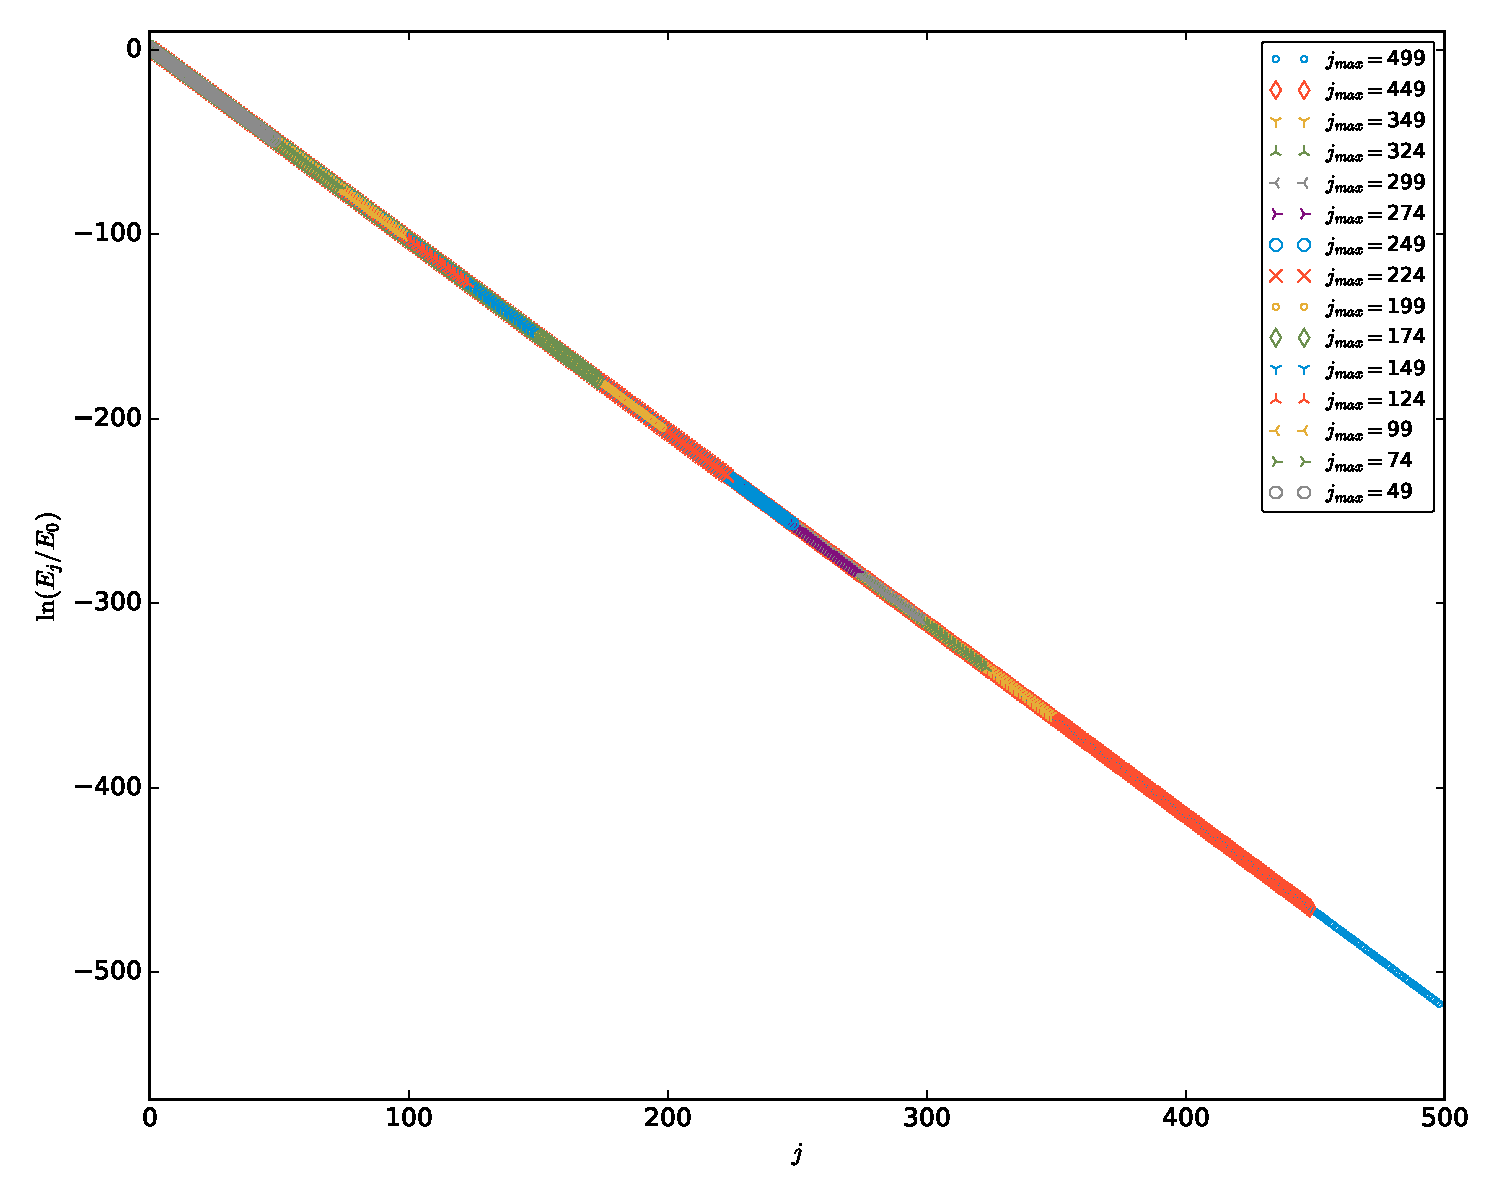
\includegraphics[width=\textwidth]{/Users/bradc/Research/Thesis/PhD/Chapter2/figs/a020_overlay_4paper}
		\caption[The smooth continuation of a low temperature QP solution from $\jm = 50$ to $\jm = 500$]{An overlay of QP solutions with $\alpha_1 = 0.2$, corresponding to $T \simeq 3.146$, for increasing values of $\jm$.}
		\label{fig: a0.2solns}
	\end{subfigure}
	\hfill
	\begin{subfigure}[t]{0.47\textwidth}
		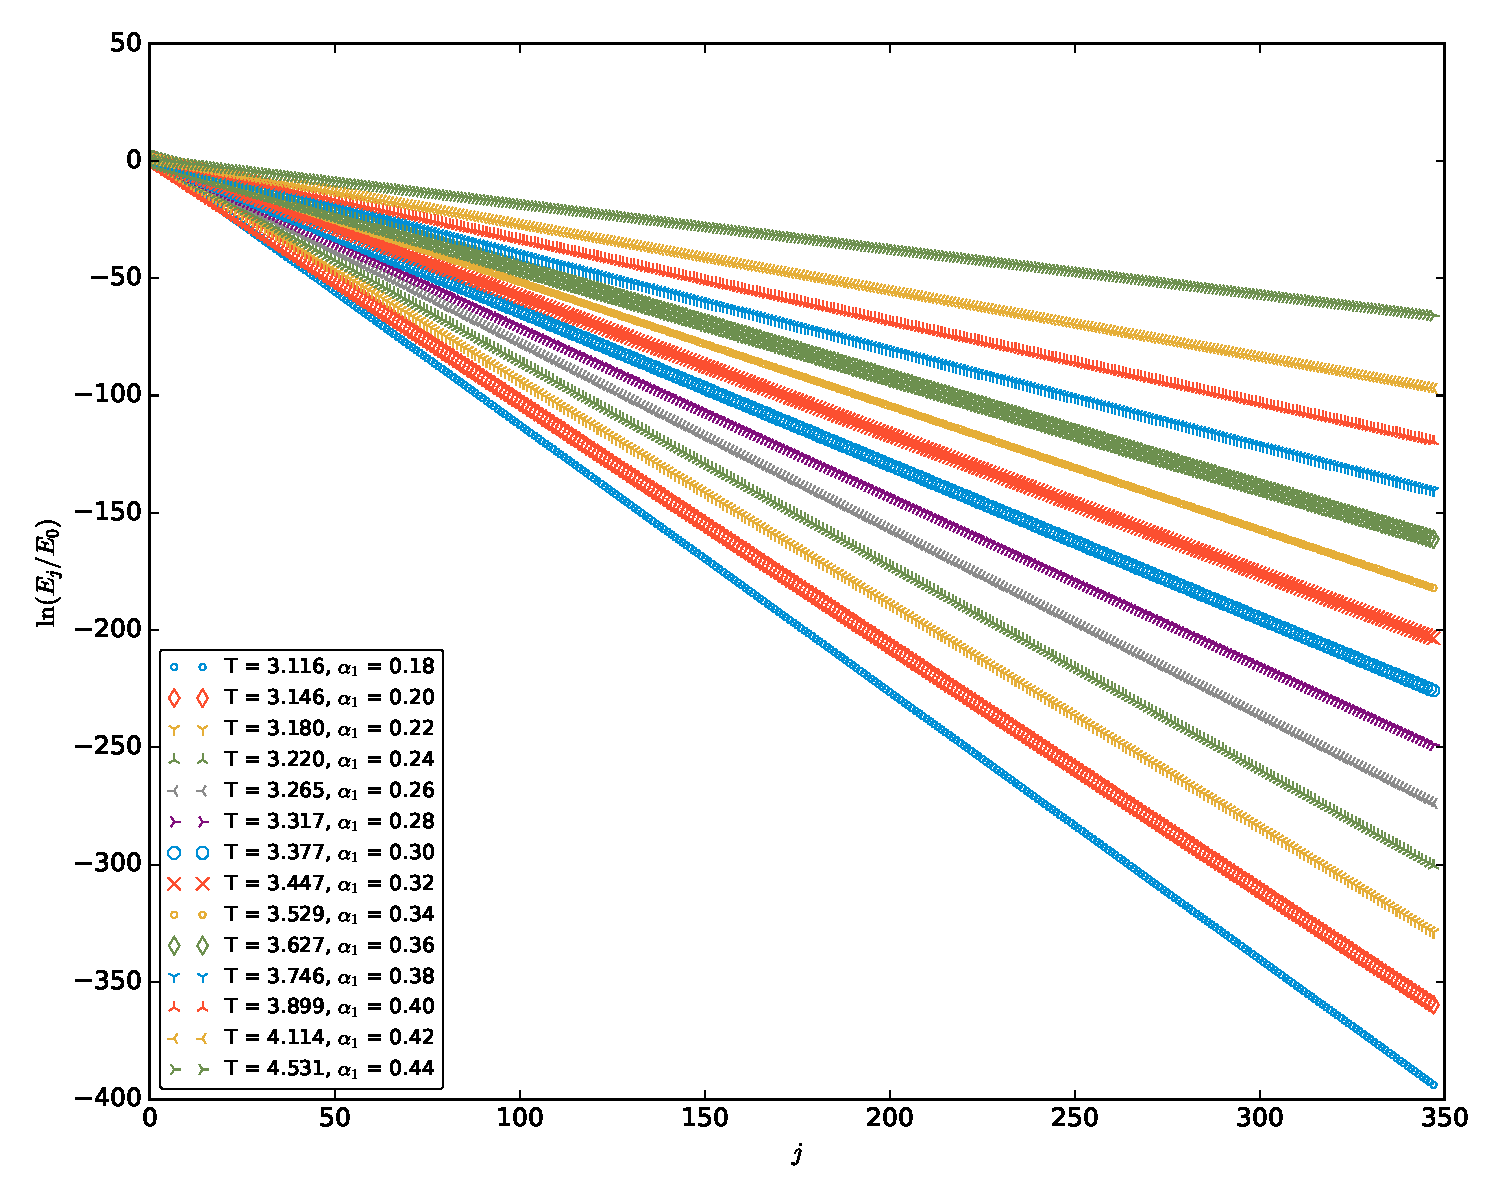
\includegraphics[width=\textwidth]{/Users/bradc/Research/Thesis/PhD/Chapter2/figs/j350_solutions_4paper}
		\caption{QP solutions with ${j_{max} = 350}$ spanning temperatures of ${3.116 \lesssim T \lesssim 4.531}$.}
		\label{fig: j350 solutions}
	\end{subfigure}
	\caption[Energy spectra for various low-$T$ QP solutions]{Energy spectra for various low temperature QP solutions.}
\end{figure}

When examining the range of $\alpha_1$ values that yield low temperature QP solutions, it was found that any small $j_{max}$ QP solution could be extended to large $j_{max}$ with proper seeding and sufficient computing power; that is, there seem to be no solutions that exist at low $j_{max}$ that cease to exist at high $j_{max}$. However, a hard limit exists at the maximum $\alpha_1$ value of $\alpha_1=0.442$, corresponding to a temperature of $T \simeq 4.643$. Above this limit, no QP solutions can be found by directly solving \eqref{qp eqn}, even with $j_{max}$ values as low as $j_{max}=50$. Conversely, there is no lower limit to $\alpha_1$ values; as $\alpha_1 \to 0$ with $\alpha_j > \alpha_{j+1}$, the TTF solution approaches the well-known single-mode solution.

%%%%%%%%%%%%%%%%%%%%%%%%%%%%%%%%%%%%%%%%%
%%%%%%%%%%%%%%%%%%%%%%%%%%%%%%%%%%%%%%%%%

\section{High Temperature Perturbations}
\label{ssec: highT}

In \cite{1507.08261}, additional QP solutions were found by repeatedly perturbing away from existing solutions: the addition of some energy $\delta E$ corresponds to the changes $\alpha_j \to \alpha_j + u_j$ and $\beta_j \to \beta_j + \theta_1 + \omega_j \theta_2$. The perturbed quantities are given by the system of linear equations
\begin{align}
\label{HT1}
\delta E &= 4 \sum_j \omega^2_j \alpha_j u_j \\
\label{HT2}
\delta N &= 4 \sum_j \oj \alpha_j u_j = 0 \\
\label{HT3}
0 &= \ol \left( \alpha_\ell (\theta_1 + \ol \theta_2) +\beta_\ell u_\ell \right) + 6T_\ell \alpha_\ell^2 u_\ell + 2 \sum_{i \neq \ell} R_{i\ell} (\alpha_i^2 u_\ell + 2 \alpha_i \alpha_\ell u_\ell ) \nonumber \\
& + 2 \stackrel{\ell \leq i + j}{\sum_{i \neq \ell} \sum_{j \neq \ell}} S_{ij(i+j-\ell)\ell} \left[ u_i \alpha_j \alpha_{i+j-\ell} + u_j \alpha_i \alpha_{i+j-\ell} + \alpha_i \alpha_j u_{i+j-\ell} \right].
\end{align}
Therefore, by solving \eqref{HT1}-\eqref{HT3} for $\{ u_j, \theta_1, \theta_2 \}$, the existing QP solution can be updated and the process can be repeated. 

For a standard QP solution with $\alpha_1 = 0.2$, the initial temperature is $T \simeq 3.146$. By applying the high temperature perturbation method described above, we are able to increase the temperature of the solution. However, this process must be examined with some scrutiny; applying repeated perturbations to a known solution does not guarantee the final result remains a valid solution. To investigate this further, we have implemented two high temperature solvers, both of which increment the energy of the system using \eqref{HT1}-\eqref{HT3} and are able to use the updated values of $\alpha_j$ and $\beta_j$ as seeds to solve \eqref{qp eqn} using a Newton-Raphson solver.

The projection used by the first solver follows the form used in \cite{1507.08261} and takes an input $\alpha_1$ value when projecting to the QP solution surface, while the second holds the temperature of the solution fixed during projection. To hold the temperature fixed, we use the definition of $T$ and the freedom to rescale the $\alpha_j$ such that $\alpha_0 = 1$ to solve for $\alpha_1$ via
\begin{align}
\label{a1 eqn}
\alpha_1^2 = \frac{1}{\omega_1 (T - \omega_1)} \left( \omega_0 (\omega_0 - T) + \sum_{j \geq 2} \omega_j (\omega_j - T) \alpha_j^2 \right)
\end{align}
It can easily be seen that $\alpha_1$ will become singular when $T = \omega_1 = 5$ in AdS$_4$. Since we are inputting a value for the temperature $T$ instead of a $\alpha_1$, we are still solving a system of $j_{max} + 1$ equations for $j_{max} + 1$ unknowns.

%%%%%%%%%%%%%%%%%%%%%%%%%%%%%%%%%%%%%%%%%

\subsection{Projections at Constant $\alpha_1$}
\label{ssec: a1 projections}

Let us first consider the results of the $\alpha_1$ projection method, shown in figure~\ref{fig: reop comparisons}. We have fixed the perturbation amount $\delta E$ to $1\%$ of the energy of the initial solution. Beginning with an $\alpha_1 = 0.44$ solution with low $\jm$, we apply repeated energy perturbations and project back to the QP solution surface with a frequency of once per 5 temperature iterations (see appendix~\ref{app: reop freq} for further discussion  on projection frequency and energy perturbation value). Figure~\ref{fig: a_1andTa0.2reop5} shows the resulting values of $\alpha_1$ and $T$ during these perturbations. We see that $\alpha_1$ approaches an attractor solution of $\alpha_1 \simeq 0.43$ with $T \simeq 4.3$. The energy perturbations between projections are insufficient to escape this local minimum, thus repeated projections return the same solution. However, when the projection frequency is decreased to once every 20 iterations, the resulting QP solution is able to bypass the attractor solution (variations of the projection frequency and energy perturbations are discussed in appendix~\ref{app: reop freq}). Note that as the iteration number increases, we actually see a \emph{decrease} in $\alpha_1$ value while the temperature continues to increase. At iteration 150 in figure~\ref{fig: a_1andTa.2reop20}, there is a cusp in $\alpha_1$ and a discontinuity in the temperature. After several hundred iterations, $\alpha_1$ becomes negative.

\vspace{0.15in}

\begin{figure}[ht]
	\centering
	\begin{subfigure}[t]{0.47\textwidth}
		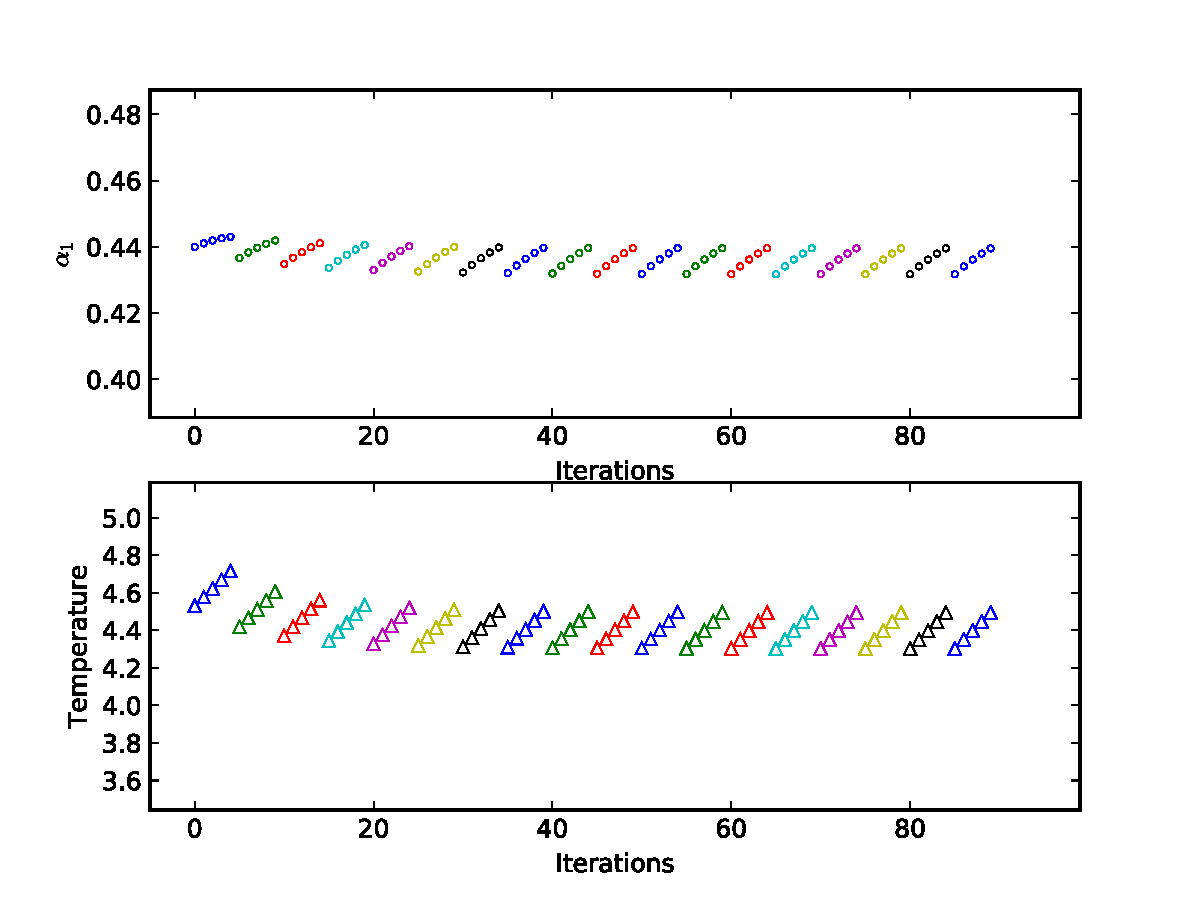
\includegraphics[width=\textwidth]{/Users/bradc/Research/Thesis/PhD/Chapter2/figs/a_1andTvsIteration_reop5}
		\caption{Applying repeated energy perturbations to an initial QP solution with $\alpha_1=0.44$, then projecting back to the QP surface every five iterations.}
		\label{fig: a_1andTa0.2reop5}
	\end{subfigure}
	\hfill
	\begin{subfigure}[t]{0.47\textwidth}
		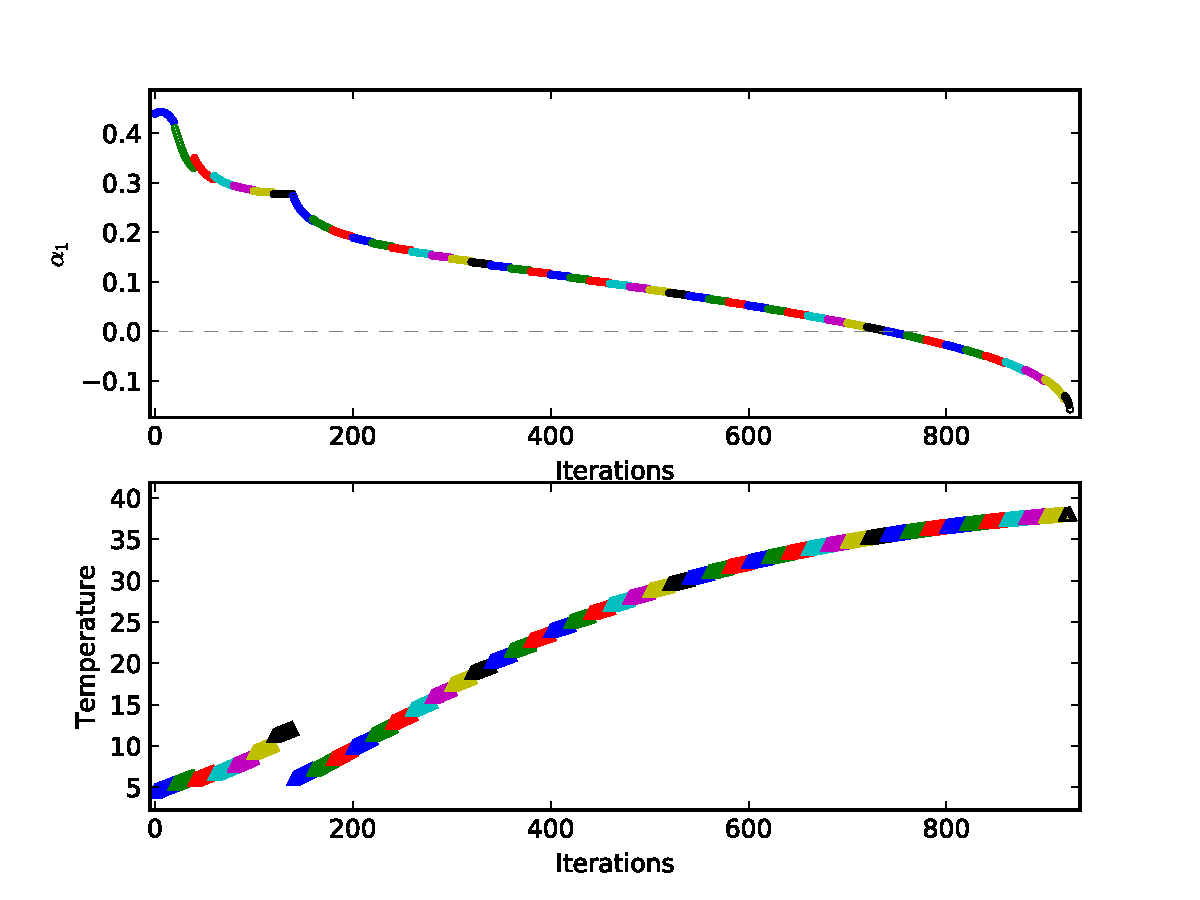
\includegraphics[width=\textwidth]{/Users/bradc/Research/Thesis/PhD/Chapter2/figs/a_1andTvsIteration_reop20}
		\caption{Beginning with the same $\alpha_1 = 0.44$ QP solution, the same process of energy perturbations are applied, this time projecting back to the QP surface every 20 iterations.}
		\label{fig: a_1andTa.2reop20}
	\end{subfigure}
	\caption[High temperature solutions resulting from projecting back to the QP solution surface at various frequencies]{The results of projecting a $j_{max}=50$, $\alpha_1 = 0.44$ solution back to the QP surface at various frequencies during high temperature perturbations. Colour changes indicate that the solution has been projected back to the QP surface.}
	\label{fig: reop comparisons}
\end{figure}

Let us examine the energy spectra of these solutions. In figure~\ref{fig: spec comparisons reop5} we see that when we choose a high projection frequency, the resulting energy spectra do not deviate far from the initial solution (using the $\alpha_1$ projection method) in either shape or temperature, but rather approach an attractor solution. The temperature of this attractor solution is robust against increases in $\jm$, as shown in table~\ref{tab: T_thresh}.

\begin{table}[h]
	\centering
	\begin{tabular}[t]{|c|c|c|}
		\hline
		$\jm$ & $T$ & Iterations \\ \hline
		$50$ & 4.30344575697724e+00 & $350$ \\ \hline
		$75$ & 4.30344544264076e+00 & $210$ \\ \hline
		$100$ & 4.30344544023857e+00 & $540$ \\ \hline
		$150$ & 4.30344544024198e+00 & $280$ \\ \hline
		$200$ & 4.30344544023915e+00 & $300$ \\ \hline
	\end{tabular}
	\caption[Attractor solution temperature for different truncation values with constant projection frequency]{The temperature of the attractor solution for various $\jm$ values. Also included is the number of iterations applied (projecting back to the solution surface with constant $\alpha_1$ after every five iterations).}
	\label{tab: T_thresh}
\end{table}

When the projection frequency is decreased, the solution is able to pass the attractor in temperaure. However, as seen in figure~\ref{fig: spec comparisons reop20}, projections back to the QP surface give $\alpha_1 < 0$ and an energy spectrum that is no longer a smooth\footnote{Here we appeal to the colloquial meaning of ``smooth'' instead of a strictly mathematical meaning, since $E_j$ is a function of a discrete variable.} function of $j$ ({\it c.f.} spectra of iterations 120 and 180). This in itself is not necessarily a breakdown of the quasi-periodic nature of the solution. However, upon examining the condition number of the matrix formed by \eqref{HT1}-\eqref{HT3}, we find that in fact the problem becomes ill-conditioned. This results in a absolute value of $u_i$ that is greater than $\alpha_i$; that is, the perturbative condition required to derive the system of linear equations \eqref{HT1}-\eqref{HT3} breaks down. For many prospective high-temperature solutions, this break-down of the perturbative condition is signalled by the loss of a smooth energy spectrum due to the values of $\alpha_j$ becoming negative. 

\vspace{0.1in}

\begin{figure}[H]
	\centering
	\begin{subfigure}[t]{0.47\textwidth}
		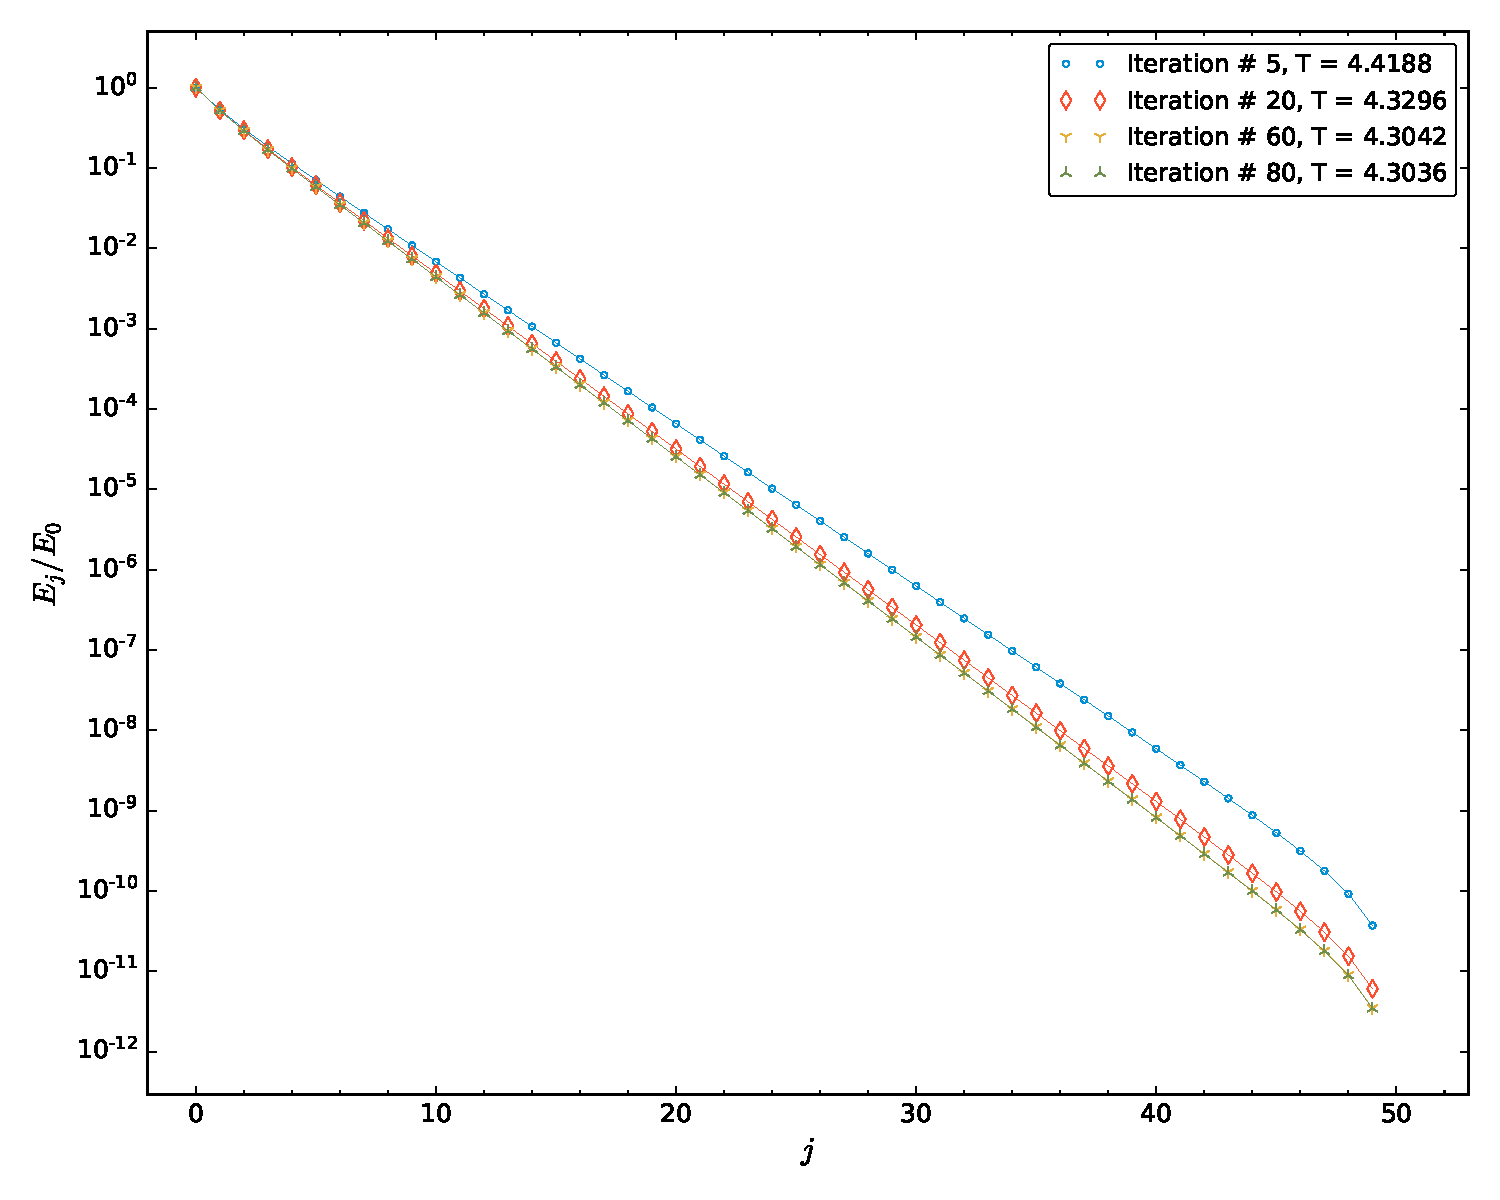
\includegraphics[width=\textwidth]{/Users/bradc/Research/Thesis/PhD/Chapter2/figs/spectracomp_a044_reop5_4paper}
		\caption{Energy spectra when projecting back to the QP solution surface every 5 iterations for an initial ${\alpha_1 = 0.44}$, QP solution (see figure~\ref{fig: a_1andTa0.2reop5} for temperature and $\alpha_1$ as a function of iteration).}
		\label{fig: spec comparisons reop5}
	\end{subfigure}
	\hfill
	\begin{subfigure}[t]{0.47\textwidth}
		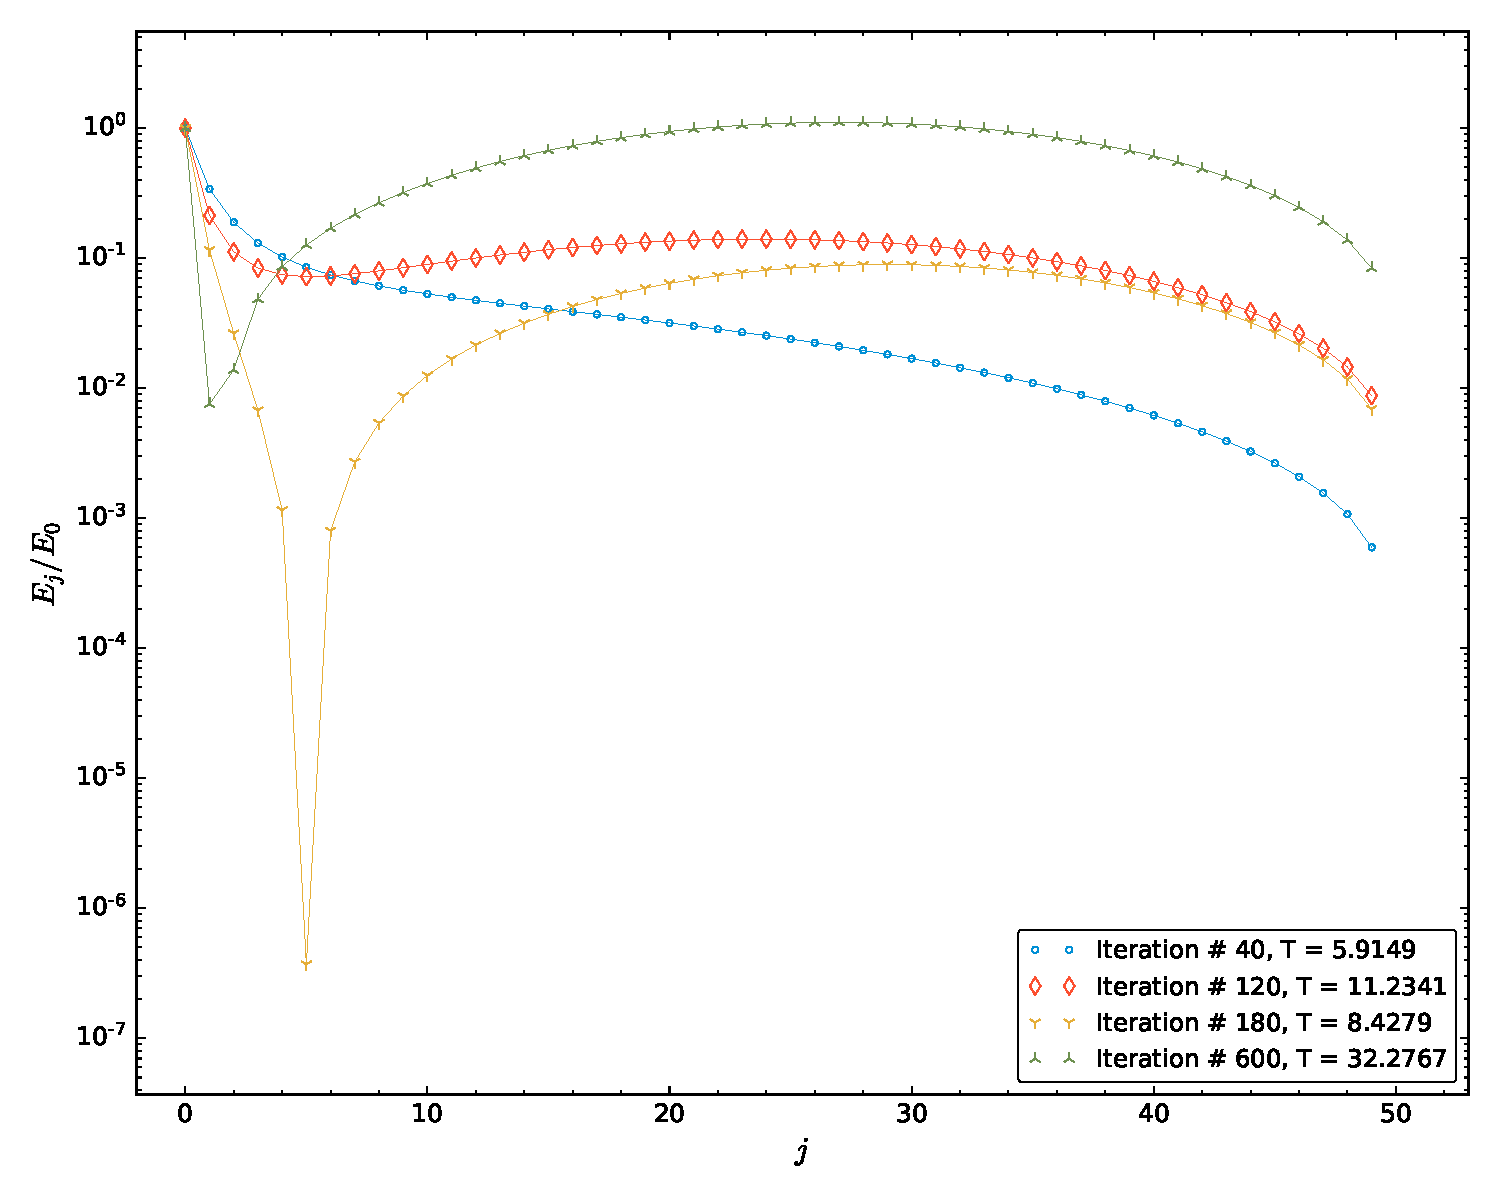
\includegraphics[width=\textwidth]{/Users/bradc/Research/Thesis/PhD/Chapter2/figs/spectracomp_a044_reop20_4paper}
		\caption{The same initial QP solution as figure~\ref{fig: spec comparisons reop5} is used, but is projected back to the QP surface every 20 iterations.}
		\label{fig: spec comparisons reop20}
	\end{subfigure}
	\caption[Energy spectra resulting from perturbing the same QP solution at differing frequencies]{Comparing energy spectra of high-temperature perturbations of an $\alpha_1=0.44$ QP solution that have been projected back to the QP surface at different frequencies.}
	\label{fig: spec comps with reop}
\end{figure}


%%%%%%%%%%%%%%%%%%%%%%%%%%%%%%%%%%%%%%%%%

\subsection{Projections at Constant Temperature}
\label{ssec: T projections}

We again use a series of small energy perturbations to seek high-temperature QP solutions, this time using a constant-temperature projection method at regular intervals. Starting from a standard $\alpha_1 = 0.44$ QP solution, we apply successive perturbations to increase the temperature. After five increments, the temperature is calculated and used as the input to the second nonlinear solver. This ensures that the temperature is not changed when projecting back to the QP solution surface. The seed values were projected back to the QP solution surface when goal temperatures of $T=5.5$, $6.0$, and $7.0$ were reached (or at the first perturbation when these temperatures were exceeded). The resulting spectra for each temperature goal over several choices of $\jm$ are shown in figure~\ref{fig: const T perturbs}. It is worth noting that we did not include the spectra for $\jm = 250$ solutions with goal temperatures of $T=6.0$ and $7.0$ because the fixed-temperature projection failed to find a solution.

\begin{figure}[tp!]
	\centering
		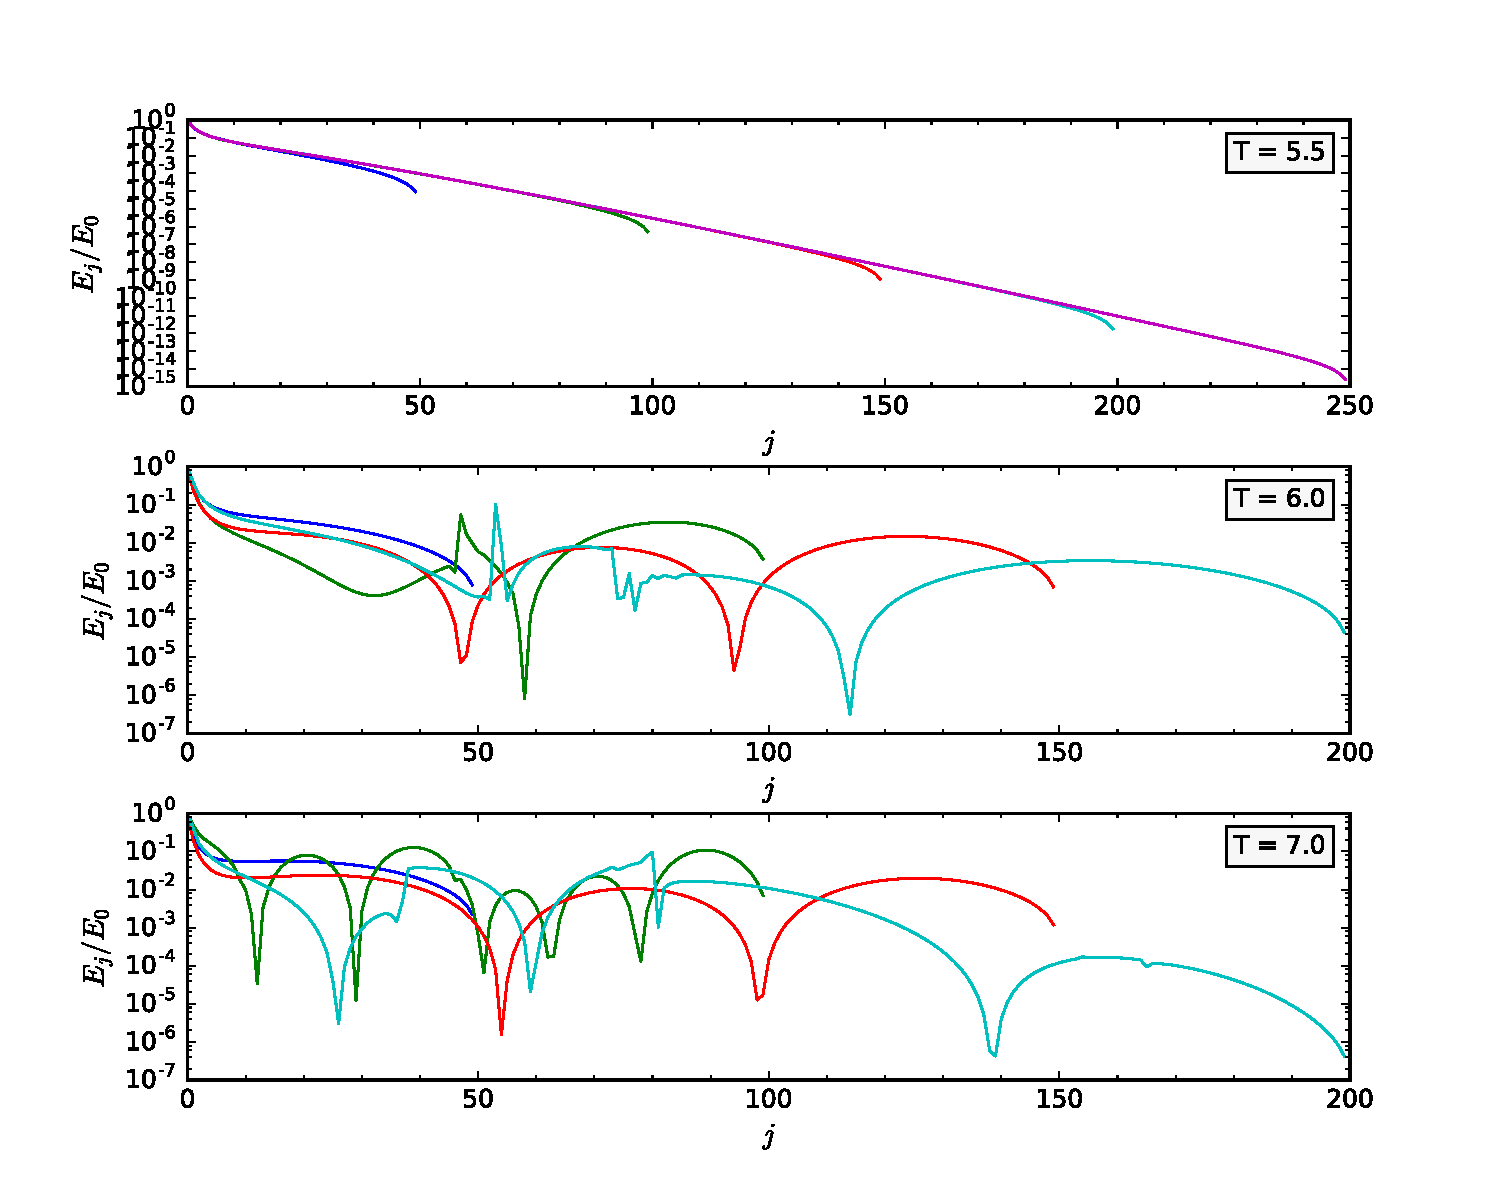
\includegraphics[width=\textwidth]{/Users/bradc/Research/Thesis/PhD/Chapter2/figs/HighTemperatureComparison}
		\caption[Finding high temperature QP solutions using repeated perturbations with regular projections back to the QP surface]{For each panel, a goal temperature (top right of plot) is set. Beginning with $\alpha_1 = 0.44$ QP solutions with ${\jm = 50, 100, 150, 200, 250}$ repeated energy perturbations are applied. After five energy perturbations, the data is projected back to the QP surface at constant $T$. When the goal temperature is either reached or exceeded for the first time, the data is again projected back at constant temperature.}
		\label{fig: const T perturbs}
\end{figure}

Recall that solutions must be robust in the limit of $\jm \to \infty$ in order to be considered solutions to the full TTF theory. While the upper panel of figure~\ref{fig: const T perturbs} suggests that solutions with temperatures at or near $T=5.5$ can be constructed in the large-$\jm$ limit, we do not find evidence that low $\jm$ solutions with $T=6.0, 7.0$ extend to the full theory.

%%%%%%%%%%%%%%%%%%%%%%%%%%%%%%%%%%%%%%%%%

\subsection{Building High-Temperature Solutions}
\label{ssec: by hand highT}

In figure~\ref{fig: const T perturbs} we see that QP solutions with smooth spectra exist for goal temperatures of $T=6.0$ and $7.0$ when $\jm = 50$ but cease being smooth as $\jm$ increases and the temperature is held constant. It is therefore reasonable to ask whether high temperature, low $\jm$ QP solutions can be extended to higher $\jm$ by using a fitting procedure to generate seed values for the fixed-$\alpha_1$ Newton-Raphson solver. In figure~\ref{fig: manual highT}, instead of fitting $\alpha_j$ values for modes ${[ j_{max} - 30, j_{max} - 10 ]}$ (as outlined in appendix~\ref{app: seeding}), we have applied the fitting method to final 5 modes and used the result to generate seed values for a solution with $\jm + 5$ modes. This method was successful in finding QP solutions with substantially higher temperatures than the previous seeding method. 

However, the solutions were not robust with the addition of extra modes. Instead, the distribution of energy in the resulting spectra becomes increasingly concentrated in {high-$j$} modes with the addition of as few as five extra modes. As we seed in figure~\ref{fig: manual highT}, fitting the tail of the $\jm = 75$, $T \simeq 27$ and producing seed values for a $\jm = 80$ solution resulted in a QP solution with $T \simeq 38$ after projecting back to the QP surface with constant $\alpha_1$. Because these solutions were not robust as $\jm$ was increased, they do not provide evidence of solutions to the untruncated theory at those temperatures.

\begin{figure}[ht]
	\centering
	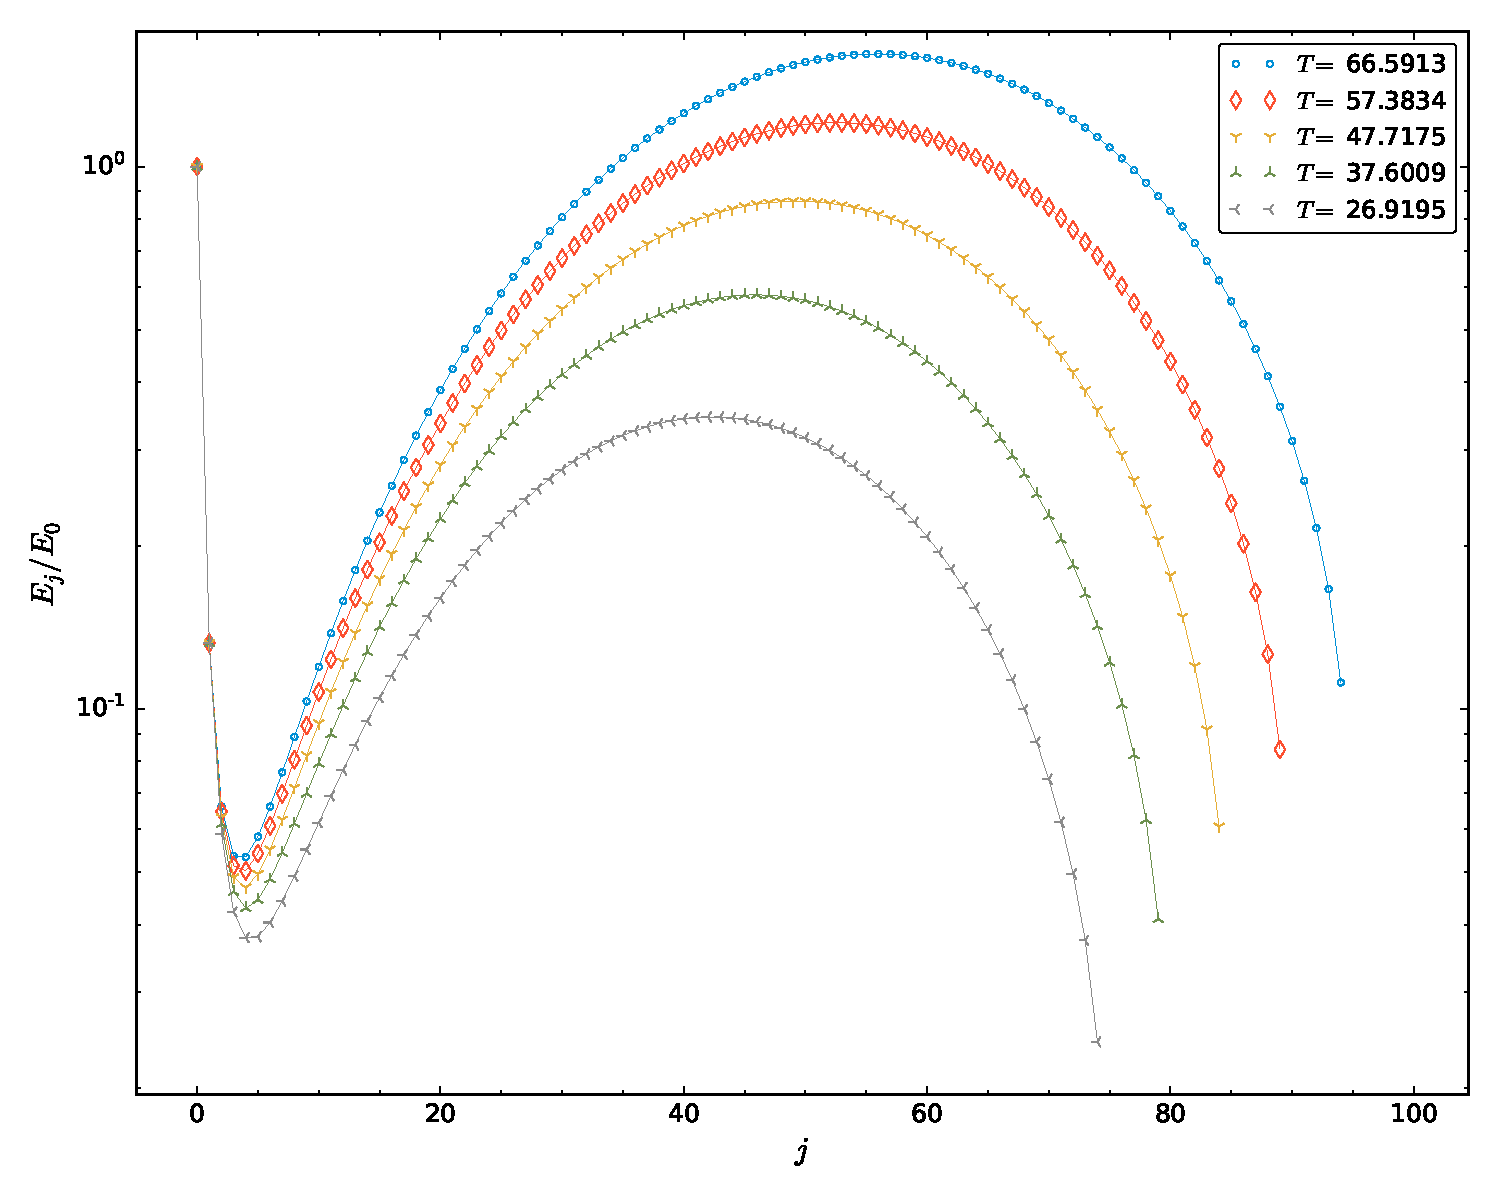
\includegraphics[width=0.75\textwidth]{/Users/bradc/Research/Thesis/PhD/Chapter2/figs/T30_extend_highj_4paper}
	\caption[Constructing high temperature solutions by hand]{Beginning with the $\jm = 75$, $T \simeq 27$ solution (grey left-tri), a fit is applied to the final five modes to generate seed values that are used in the fixed-$\alpha_1$ Newton-Raphson solver find the next QP solution. The procedure is repeated to generate the $\jm = 80$, $T \simeq 38$ (green up-tri), $\jm = 85$, $T \simeq 48$ (yellow down-tri), $\jm = 90$, $T \simeq 57$ (red diamonds), and $\jm = 95$, $T \simeq 67$ (blue circles) QP spectra.}
	\label{fig: manual highT}
\end{figure}

In \cite{1507.08261}, it was suggested that QP solutions should exist in a continuous region of temperature space ${T \in [T_{min}, T_{max}] = [d, 2\jm + d]}$. To produce high-temperature solutions, successive energy perturbations could be applied to a low-temperature solution with a low frequency of projecting back to the QP surface. However, we have found that the high temperature solutions produced using regular projections back to the solution surface are not robust as $\jm$ increases and therefore do no constitute physical solutions. In further pursuit of high temperature QP solutions, we investigated additional methods for generating these solutions.

First, we considered applying a similar fitting technique to a $T \simeq 5.4$ QP solution as that which was used to extend low-temperature QP solutions. In this case, values were taken from the middle\footnote{Typically at $\jm / 2$, where the power law scaling has not been affected by edge effects.} of high temperature solutions with $\jm = 50$ and fit with an exponential function (see figure~\ref{fig: solutionfitting} for a similar procedure with tail values) to produce 10 new modes, $\{ \alpha_{fit} \}$. We then inserted the new values $\alpha_{fit}$ with the existing data so that $\alpha_j = \langle \alpha_{j< j_{mid}}, \alpha_{fit}, \alpha_{j > j_{mid}} \rangle$. The result was to extend the data by 10 modes and slightly increase the temperature, thereby providing a good seed for the constant-temperature nonlinear solver. However, no solutions were found by the Newton-Raphson solver, starting either with $\jm = 50$, $T>5.5$ data, or $\jm = 200$, $T \simeq 5.5$ data.

Next, we considered perturbing up to an intermediate temperature $5.5 \ll T_{int} < T_{max}$ before attempting to project back to the QP surface using the $T_{int}$ data as seed values. In particular, we repeatedly perturbed a $T \simeq 4.5$ solution using the method described in \S~\ref{ssec: highT} to a temperature of $T_{int} = 20$ without projecting back to the QP surface \emph{at any point}. For $\jm \lesssim 100$, projection back to the solution surface finds a new solution with $T < T_{int}$ that -- much like the spectra shown in figure~\ref{fig: spec comparisons reop20} -- loses its smooth profile. Under evolution within the TTF theory (discussed below), the fractional energy in the low-frequency modes oscillates rapidly over several orders of magnitude during the evolution and the Ricci scalar reaches values $\mc O (10^6)$; these solutions are almost certainly not quasi-periodic. The same result is found for high-temperature solutions created by fitting tail data (see figure~\ref{fig: manual highT} for example spectra). Finally, for $\jm \geq 100$, projection back to the QP solution surface once $T = T_{int}$ fails entirely. Thus, we did not find evidence for QP solutions with temperatures above $T \simeq 5.5$.




%Despite high-temperature solutions being inaccessible via repeated energy perturbations, we may ask if such solutions can be found by using different methods. First, we consider perturbing a known QP solution to a high temperature \emph{without} regular projections back to the QP surface. Then, at some sufficiently high temperature $T_{max}$, we attempt to project back to the QP surface. In figure~\ref{fig: T30 vs j_max}, the spectra of QP solutions before and after projection are shown for increasing $j_{max}$. For solutions with $\jm \geq 100$, high-temperature solutions are in fact projected to low-temperature solutions that may contain negative $\alpha_j$ values. Low-$\jm$ solutions, however, appear to remain at high-temperatures after projecting back to the surface. We use this type of solution in our next method.
%\begin{figure}[ht]
%	\centering
%	\begin{subfigure}[t]{0.45\textwidth}
%		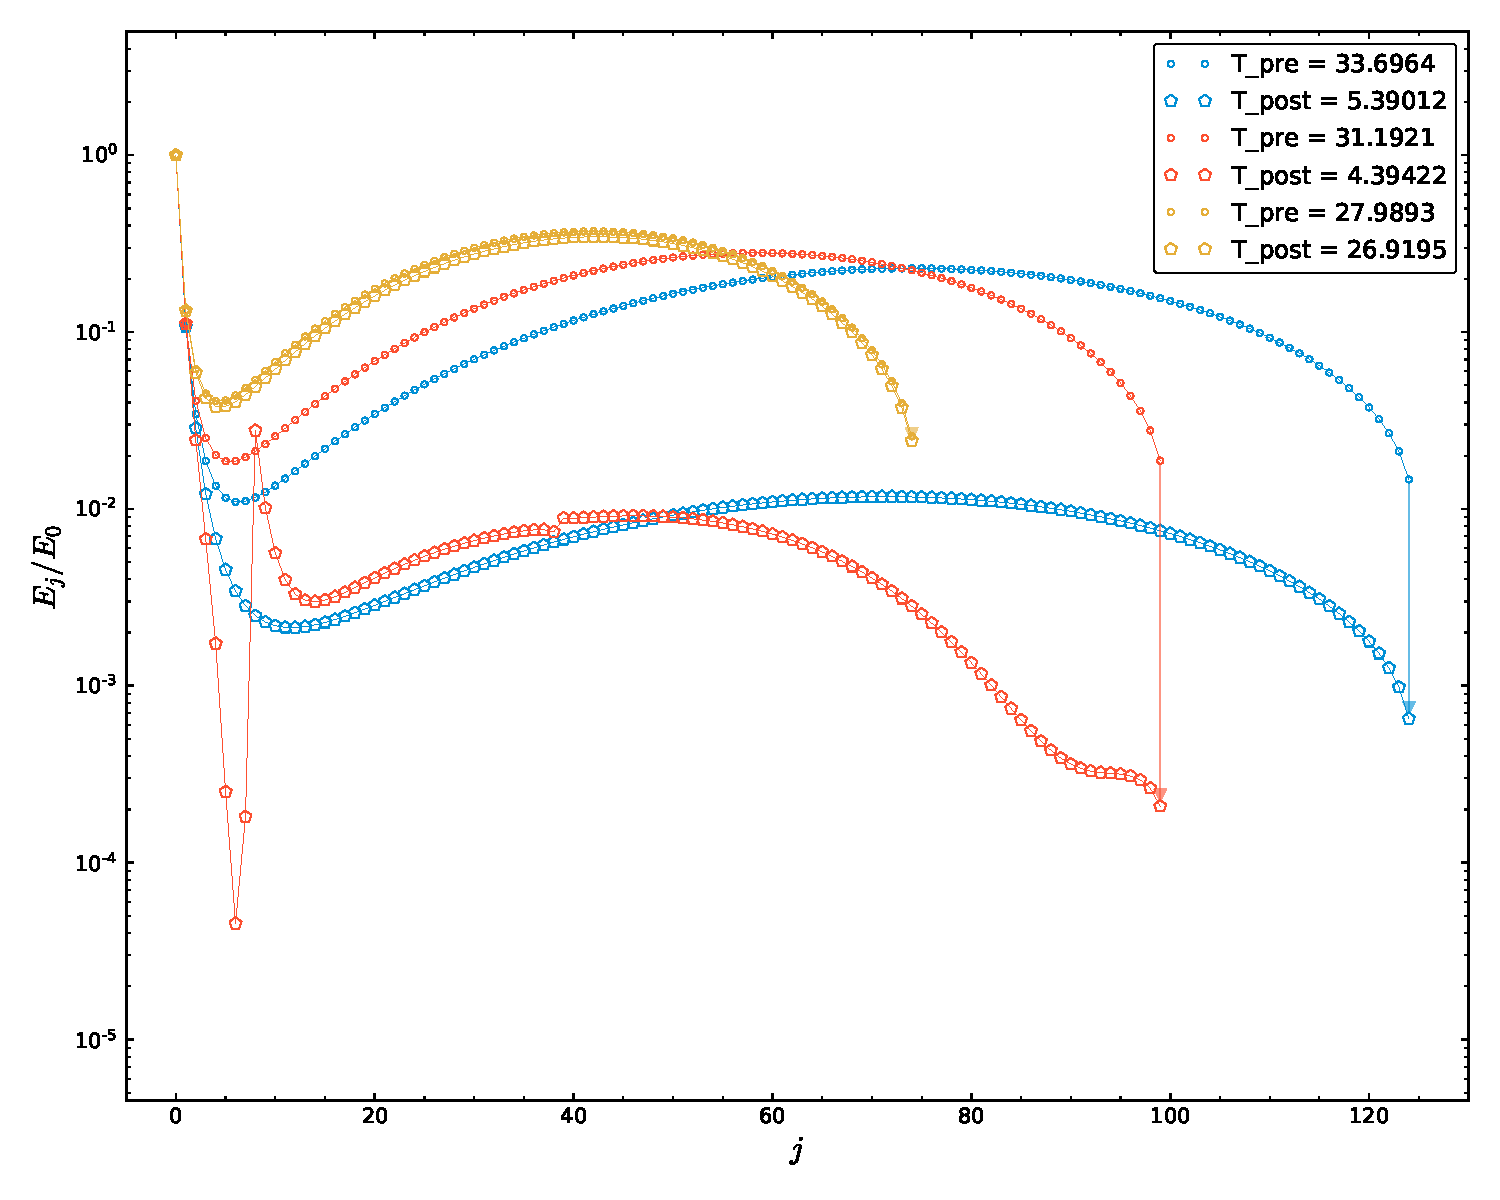
\includegraphics[width=\textwidth]{/Users/bradc/Research/Thesis/PhD/Chapter2/figs/T30vsj_max_partial_4paper}
%		\caption{QP solutions perturbed to $T_{max}=30.00$, which were then used as seeds for the nonlinear solver. Arrows are oriented from pre-optimized to post-optimized solutions.}
%		\label{fig: T30 vs j_max}
%	\end{subfigure}
%	\;
%	\begin{subfigure}[t]{0.45\textwidth}
%		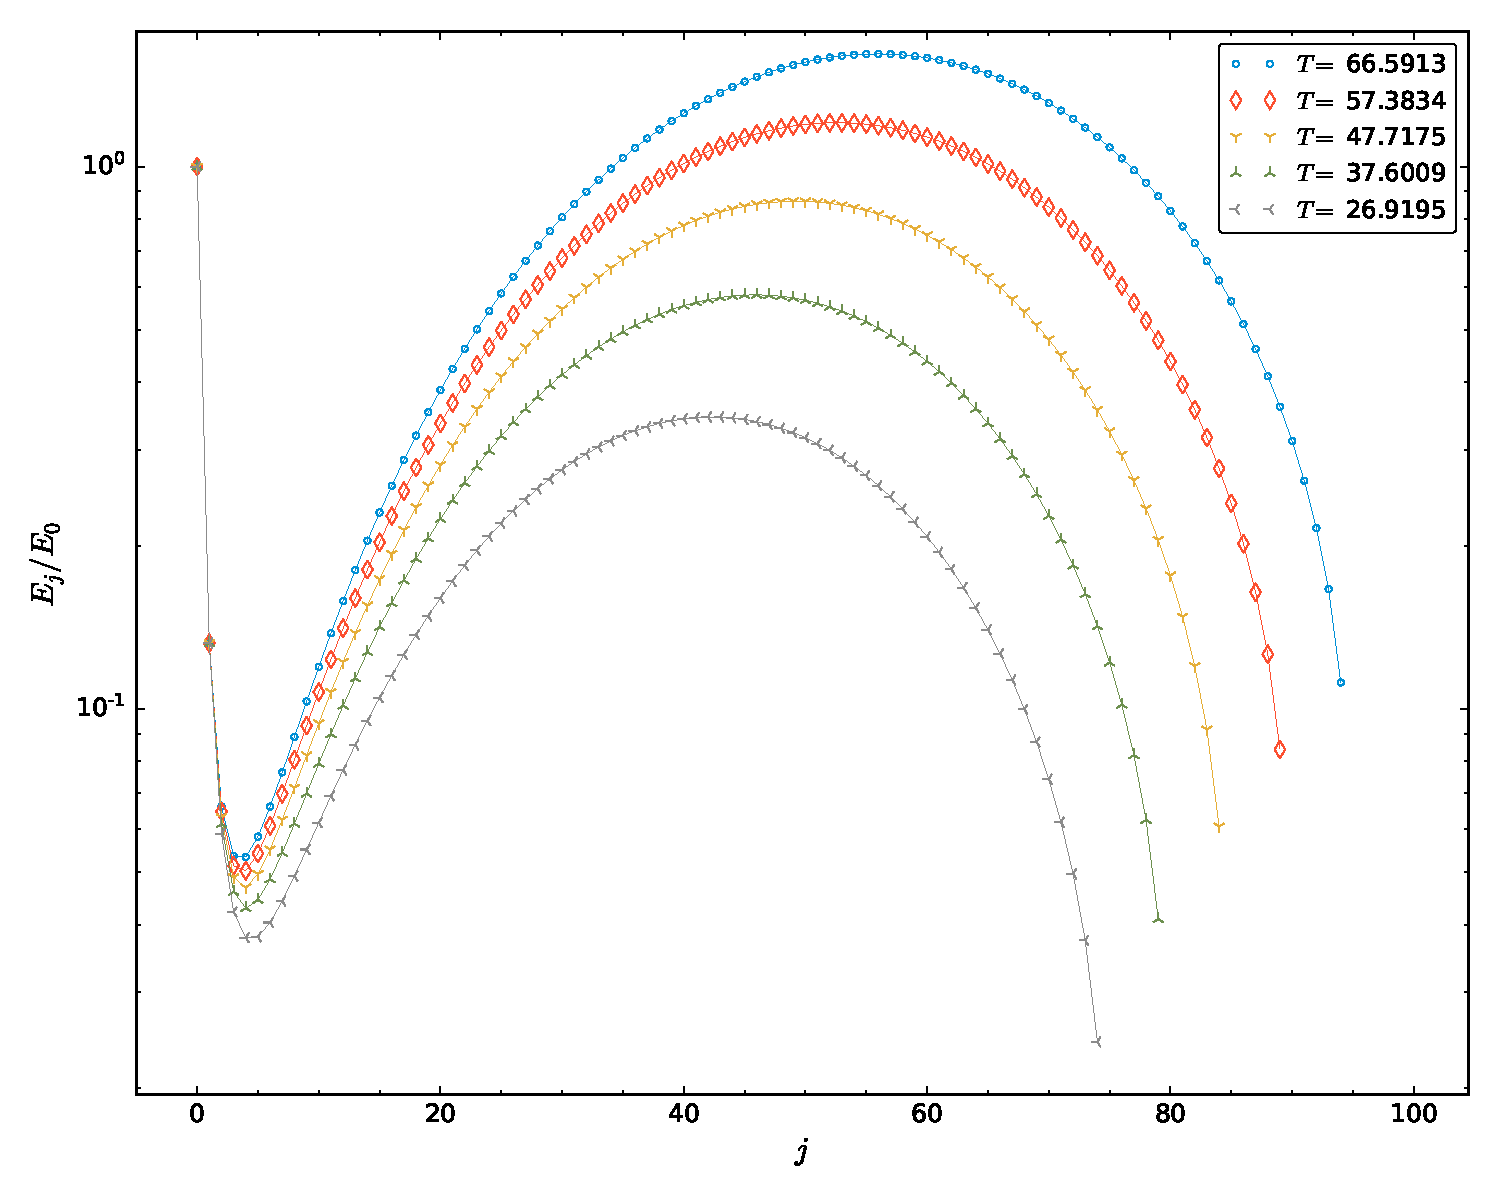
\includegraphics[width=\textwidth]{/Users/bradc/Research/Thesis/PhD/Chapter2/figs/T30_extend_highj_4paper}
%		\caption{Extensions of the $j_{max}=50$ solution from figure~\ref{fig: T30 vs j_max} to larger $j_{max}$ solutions using tail fitting on only the final 5 modes of the solution.}
%		\label{fig: manual highT}
%	\end{subfigure}
%	\caption[Constructing high temperature solutions by hand]{Constructing high temperature solutions ``by hand.''}
%	\label{fig: making highT}
%\end{figure}


%%%%%%%%%%%%%%%%%%%%%%%%%%%%%%%%%%%%%%%%%

%\begin{figure}[ht]
%	\centering
%	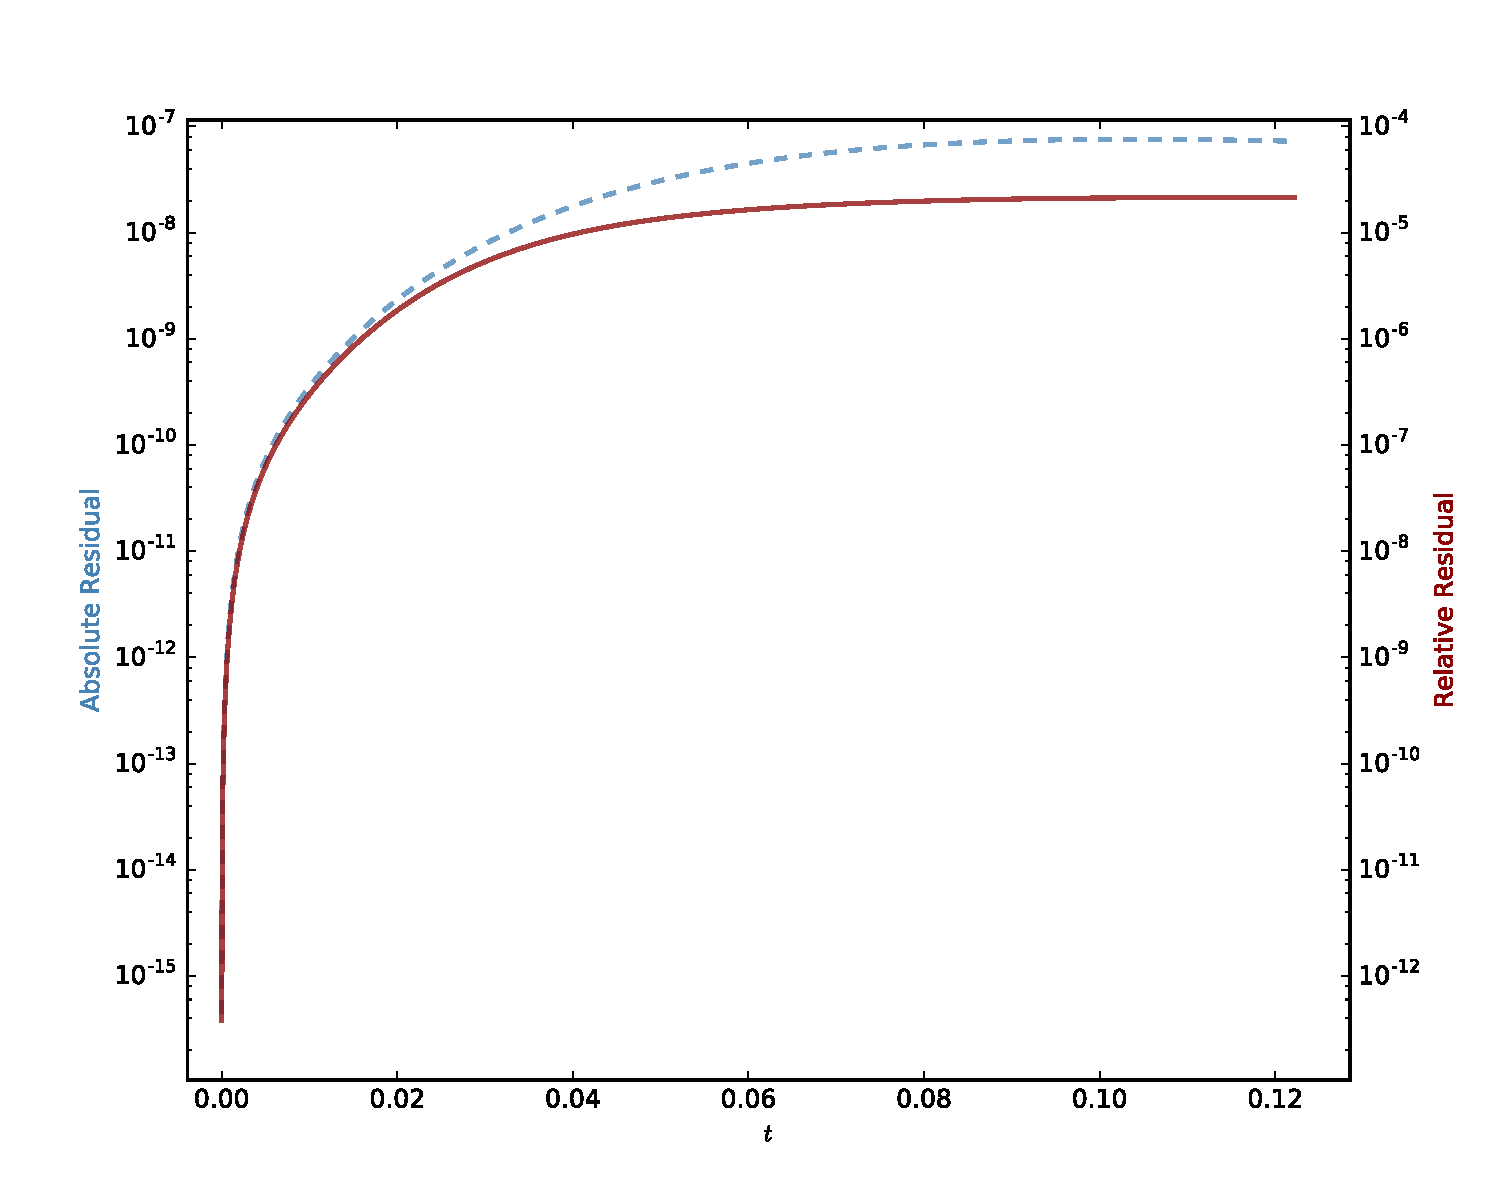
\includegraphics[0.75\textwidth]{/Users/bradc/Research/Thesis/PhD/Chapter2/figs/Qpa4_40e-01j100EEresids}
%	\caption[Absolute and relative residuals for a low-temperature QP solution]{Absolute and relative residuals during evolution of a low-temperature, $\jm = 100$ QP solution with $\epsilon = 0.001$.}
%	\label{fig: qpEEresids}
%\end{figure}

%%%%%%%%%%%%%%%%%%%%%%%%%%%%%%%%%%%%%%%%%
%%%%%%%%%%%%%%%%%%%%%%%%%%%%%%%%%%%%%%%%%

\section{Time Evolution of Quasi-Periodic Solutions}
\label{sec: time evolution}

The weakly turbulent behaviour of the scalar field in the TTF is captured by the $\mc O(\epsilon^2)$ renormalization group flow equations {\eqref{RN1}-\eqref{RN2}}. Having identified different families of quasi-periodic solutions, we wish to evolve these solutions within the TTF description. Furthermore, we may also be able to identify previously inaccessible solutions by evolving a QP solution within the TTF framework before attempting to project back to the QP surface. To achieve these aims, we use numerical methods first described by \cite{1606.02712} and take both low-temperature and high-temperature QP solutions as initial data. 

%%%%%%%%%%%%%%%%%%%%%%%%%%%%%%%%%%%%%%%%%

\subsection{Low-temperature QP data}

Let us consider the evolution of a ``typical'' QP solution: a solution to \eqref{qp eqn} with $\alpha_1 = 0.2$ and $\jm = 100$, corresponding to a temperature of $T \simeq 3.146$. Choosing an amplitude of $\epsilon = 0.01$ (note that the TTF equations are invariant under $\mc A(\tau) \to \epsilon \, \mc A(\tau / \epsilon^2)$ and so the value of $\epsilon$ does not change the physics), figure~\ref{fig:qpevo} shows the evolution of the fraction of the total energy per mode. We see that energy in the lowest-$j$ modes remains constant over the duration of the evolution, while the fraction in the highest-$j$ modes increases after $t \simeq 300$. Similar behaviour is observed for higher $\jm$ solutions and over values of $0.2 \leq \alpha_1 \leq 0.44$. Given the scale of the energy in the modes $j \geq 96$, the growing energy fractions in these modes can mainly be attributed to numerical errors rather than direct energy cascades.

\begin{figure}[H]
	\centering
	\begin{subfigure}[t]{0.47\textwidth}
		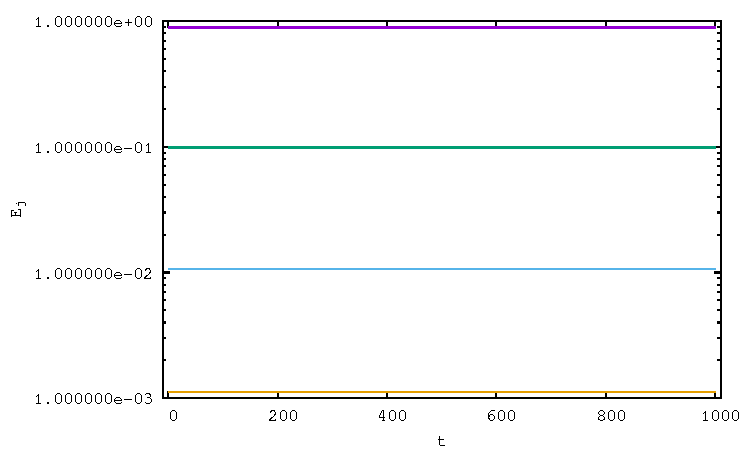
\includegraphics[width=\textwidth]{/Users/bradc/Research/Thesis/PhD/Chapter2/figs/QPa2_00e-01_j100_lowjenergyevo}
		\caption{From top to bottom: $j=0, 1, 2, 3$ (purple, green, blue, orange).}
	\end{subfigure}
	\hfill
	\begin{subfigure}[t]{0.47\textwidth}
		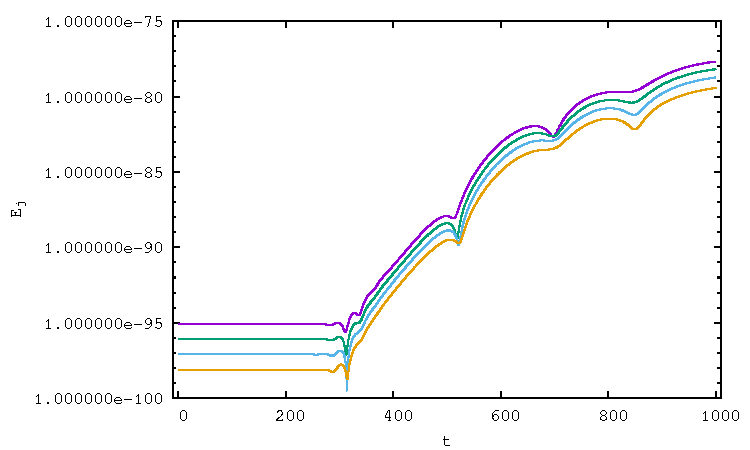
\includegraphics[width=\textwidth]{/Users/bradc/Research/Thesis/PhD/Chapter2/figs/QPa2_00e-01_j100_highjenergyevo}
		\caption{From top to bottom: $j=96, 97, 98, 99$ (purple, green, blue, orange).}
	\end{subfigure}
	\caption[Evolution of QP solutions at low temperature]{Fraction of the total energy in each mode during evolution of an $\alpha_1 = 0.2$, $\jm = 100$, QP solution with $\epsilon=0.01$.}
	\label{fig:qpevo}
\end{figure}

%To better understand how well such solutions continue to satisfy the TTF equation throughout their time evolution, we evaluate the residuals of \eqref{qp eqn} at regular intervals of $t=0.025$ during the evolution of a $\jm = 100$, $T=4.531$ QP solution using data taken during the evolution. Figure~\ref{fig: Qpa4_40e-01QPresids} is a sample of the $L^2$-norm of these residuals for 

%\begin{figure}[ht]
%	\centering
%	\begin{subfigure}[t]{0.45\textwidth}
%		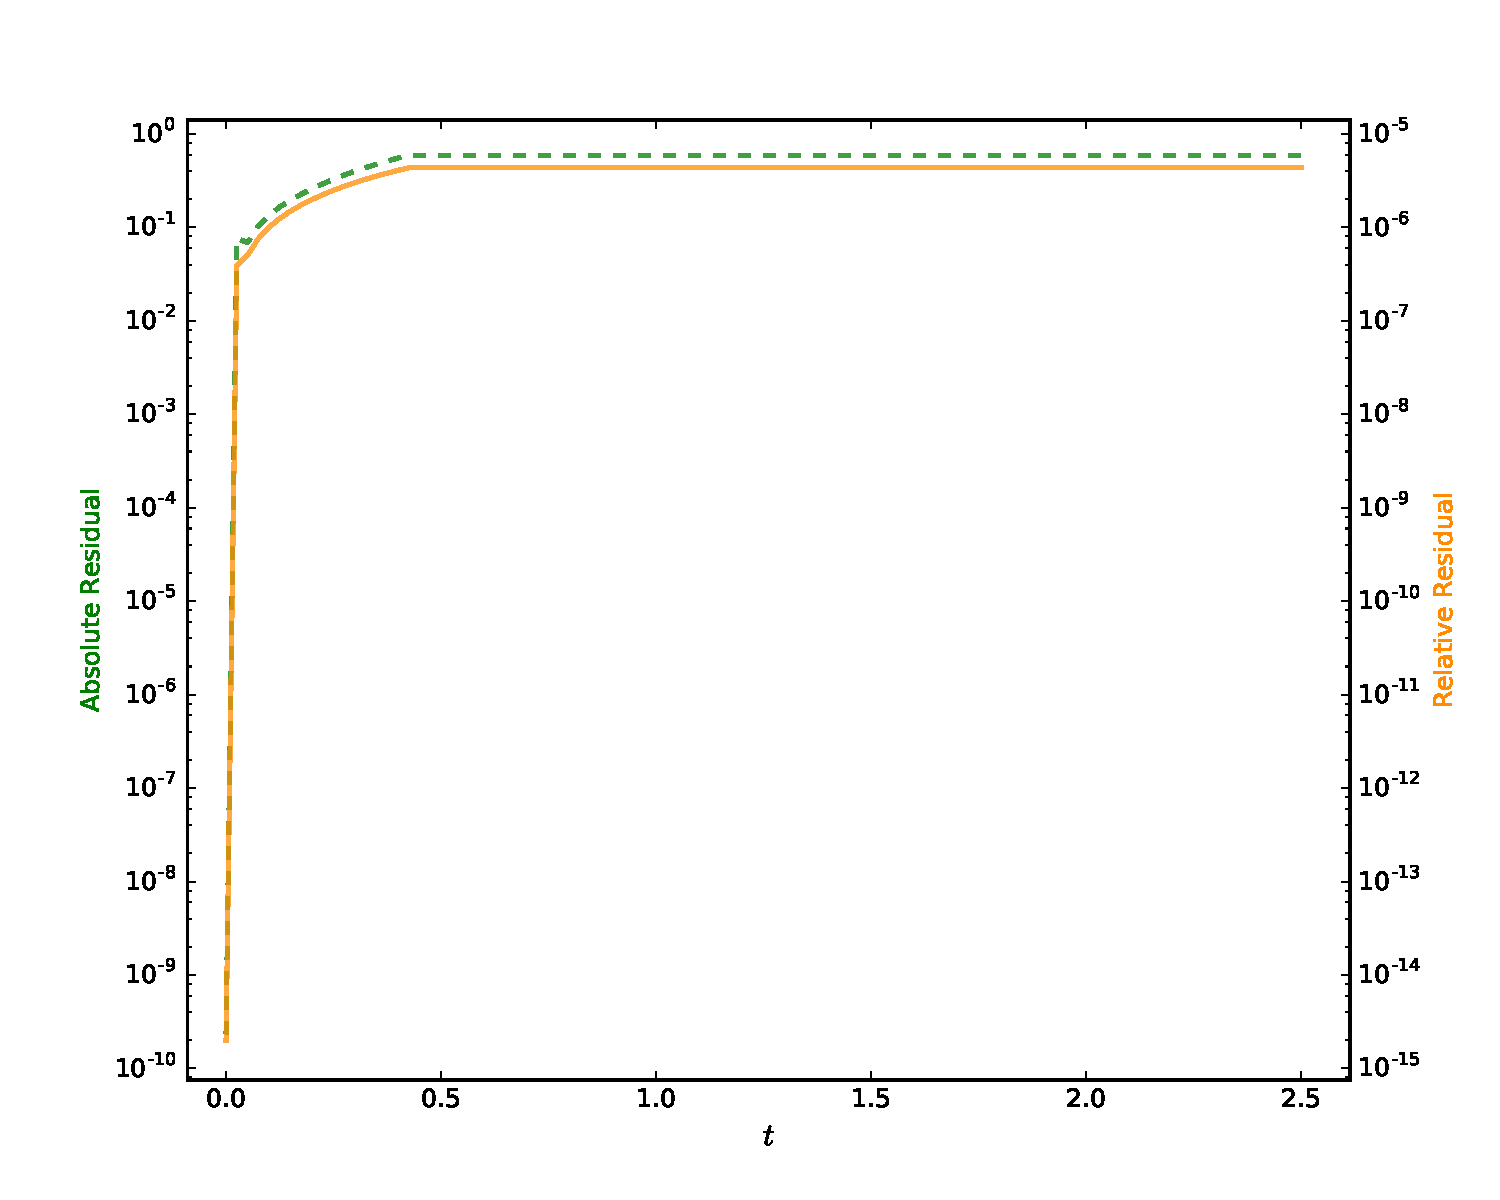
\includegraphics[width=\textwidth]{/Users/bradc/Research/Thesis/PhD/Chapter2/figs/Qpa4_40e-01QPresids}
%	\end{subfigure}
%	\;
%	\begin{subfigure}[t]{0.45\textwidth}
%		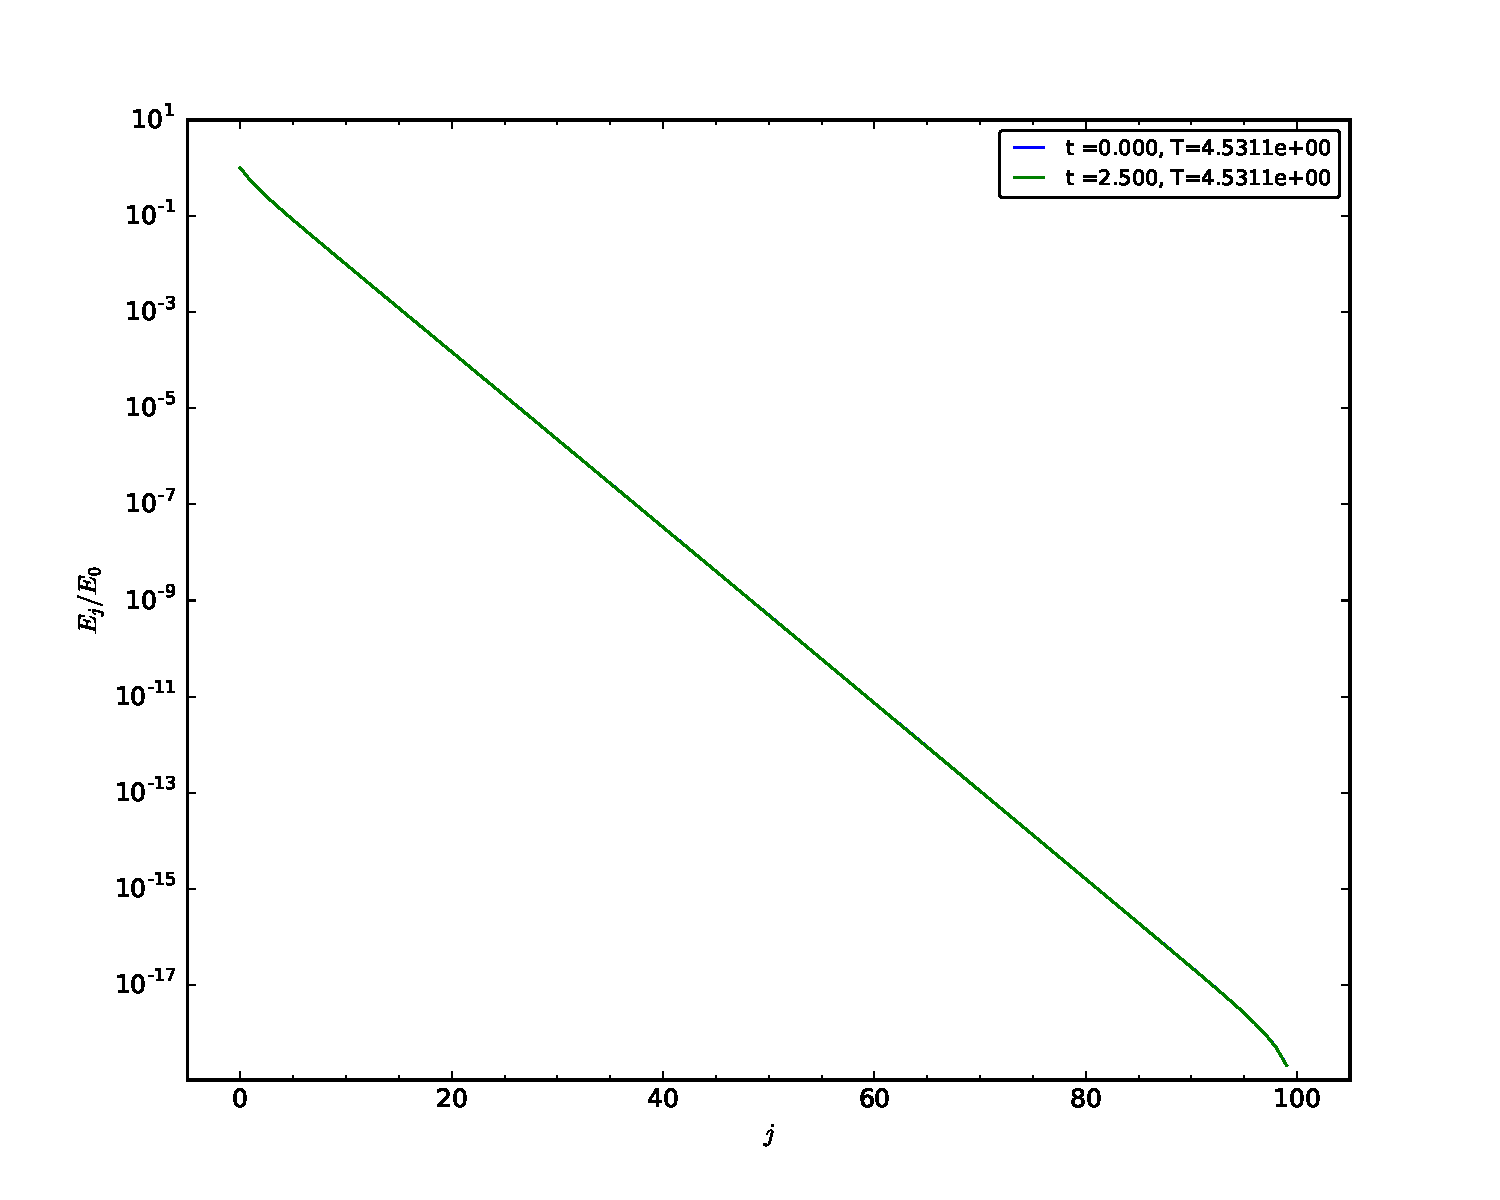
\includegraphics[width=\textwidth]{/Users/bradc/Research/Thesis/PhD/Chapter2/figs/Qpa4_40e-01specevo}
%	\end{subfigure}
%	\caption[Residual and spectrum of a low-temperature QP solution during evolution]{{\it Left:} $L^2$-norm of the residuals of \eqref{qp eqn} evaluated at intervals of $0.025$ during the evolution of a $\jm = 100$, $\alpha_1 = 0.44$ QP solution with $\epsilon = 0.1$. {\it Right:} The spectra of the QP solution at the beginning and end of the evolution.}
%	\label{fig: Qpa4_40e-01QPresids}
%\end{figure}

We may also ask: does a given quasi-periodic solution remain unique under evolution? That is, will the solution project back to itself during its evolution? To answer this, we evolve the same low-temperature, QP solution and take the spectra at different times as seed values for projecting back to the QP surface. We see that seed values taken from data with $t > 0$ are projected back to themselves (using the constant $\alpha_1$ Newton-Raphson method) at all times during the evolution, and that the resulting solutions solve the QP equation \eqref{qp eqn} to a high degree of accuracy (see figure~\ref{fig: Qpa4_40e-01j100EvolutionProjection}). 

%While this is to be expected for such low-temperature QP solutions, we will soon see that even padding a known QP solution with zeros causes the loss of quasi-periodicity during evolution. For comparison, figure~\ref{fig: QPa4_40e-01padj200_evolutionprojection} shows the results of attempting to project a QP solution that has been padded with zeros back to the QP surface during its evolution. Note the scale on the plot of the $L^2$-norm in either case.

\begin{figure}[ht]
	\centering
	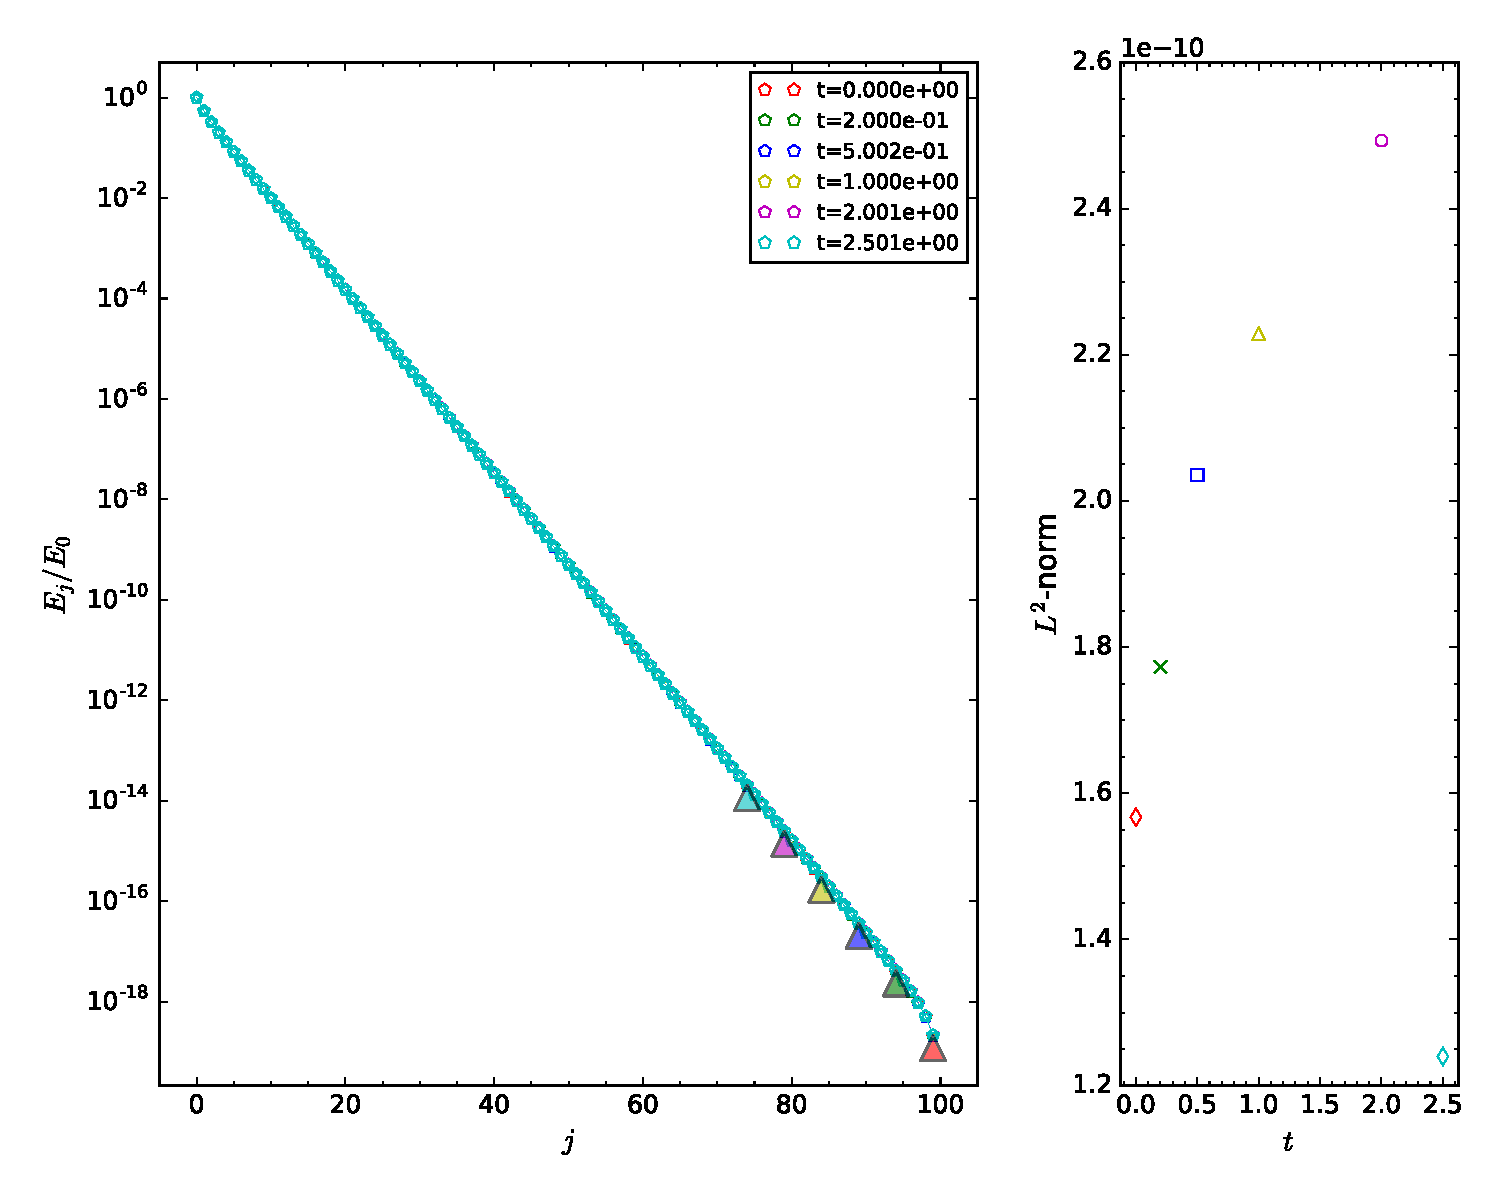
\includegraphics[width=0.6\textwidth]{/Users/bradc/Research/Thesis/PhD/Chapter2/figs/Qpa4_40e-01j100EvolutionProjectionPlot}
	\caption[Taking the spectrum of a QP solution during evolution to use as a seed to find new QP solutions]{Left: Projecting a low-temperature solution back to the QP surface with constant $\alpha_1$ during its evolution. Arrows are oriented from amplitude/phase seed values (circles) to QP surface projections (pentagons). Right: the $L^2$-norms of the errors between  solutions at $t\simeq 0.0, 0.2, 0.5, 1.0, 2.0, 2.5$ (red diamond, green cross, blue square, yellow triangle, magenta circle, blue diamond).}
	\label{fig: Qpa4_40e-01j100EvolutionProjection}
\end{figure}

%\begin{figure}[ht]
%	\centering
%	\begin{subfigure}[t]{0.45\textwidth}
%		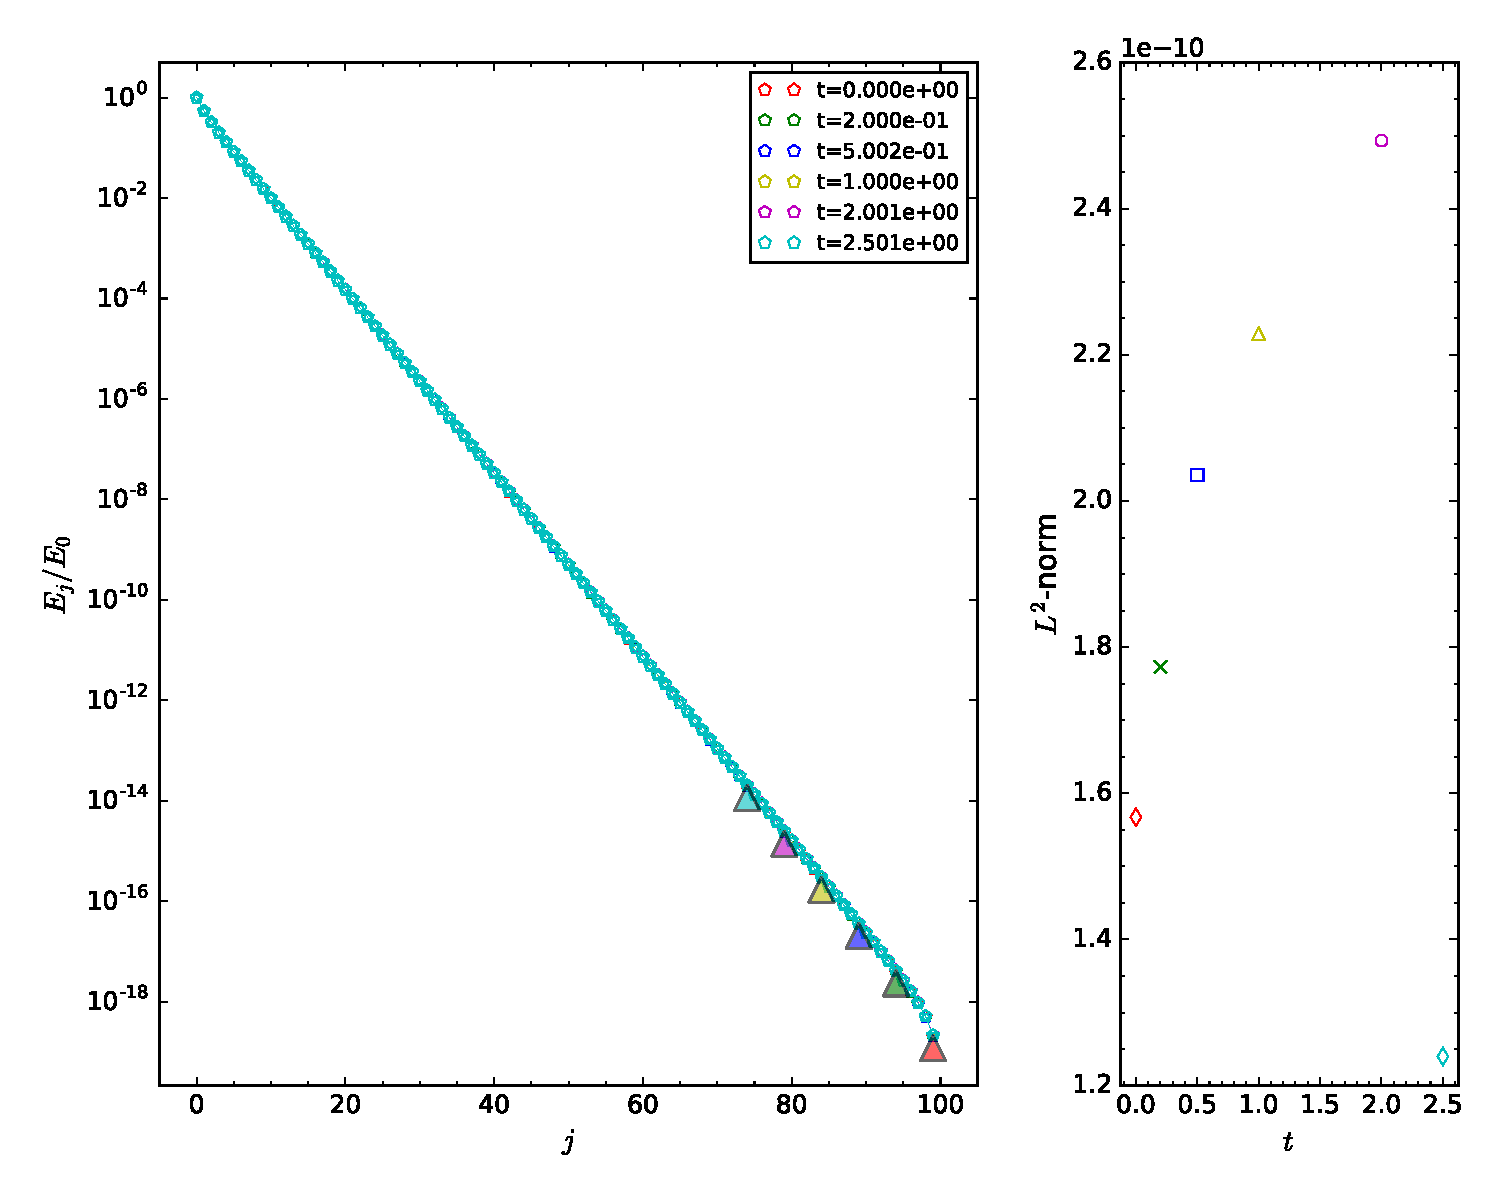
\includegraphics[width=\textwidth]{/Users/bradc/Research/Thesis/PhD/Chapter2/figs/Qpa4_40e-01j100EvolutionProjectionPlot}
%		\caption{Projected solutions for a low-temperature, QP solution and their $L^2$-norms at $t\simeq 0.0, 0.2, 0.5, 1.0, 2.0, 2.5$ (red diamond, green cross, blue square, yellow triangle, magenta circle, blue diamond).}
%		\label{fig: Qpa4_40e-01j100EvolutionProjection}
%	\end{subfigure}
%	\;
%	\begin{subfigure}[t]{0.45\textwidth}
%		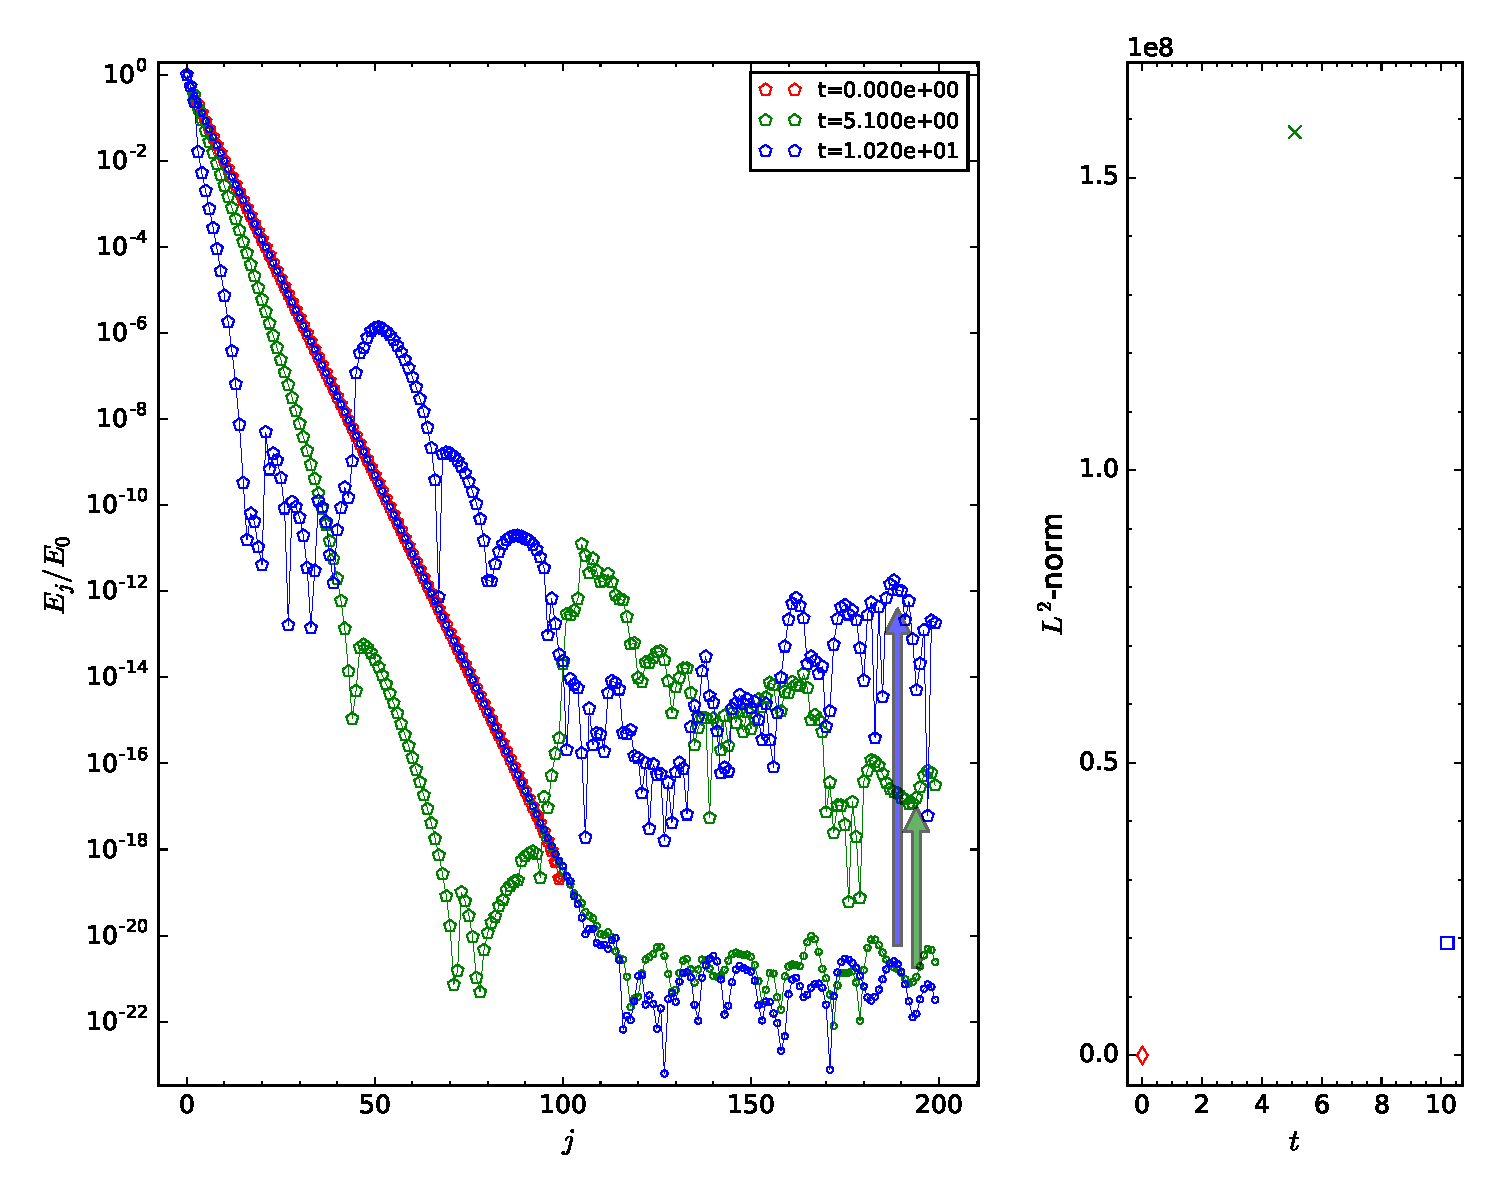
\includegraphics[width=\textwidth]{/Users/bradc/Research/Thesis/PhD/Chapter2/figs/QPa4_40e-01padj200_evolutionprojection}
%		\caption{The same QP solution is padded with zeros out to $\jm = 200$ and evolved in time. Intermediate solutions are projected back to the QP surface at $t \simeq 0.0, 5.1, 10.2, ...$ (red diamond, green cross, blue square ...)}
%		\label{fig: QPa4_40e-01padj200_evolutionprojection}
%	\end{subfigure}
%	\caption[Taking the spectrum of a QP solution during evolution to use as a seed to find new QP solutions]{Intermediate values from the amplitude/phase evolution of a solution are used as seeds for the nonlinear solver at various times. Arrows are oriented from amplitude/phase seed values (circles) to QP surface projections (pentagons).}
%\end{figure}

\vspace{-0.1in}

In an effort to find new QP solutions, we consider an alternative method for finding solutions that may not be accessible through established seeding methods. We pad a given quasi-periodic solution with extra modes that are initially set to zero and project back to the QP solution surface. Upon amplitude-phase evolution via \eqref{RN1}-\eqref{RN2}, the energy in the lower-$j$ modes will flow into the higher-$j$ modes. This may lead to new quasi-periodic solution with the same temperature but larger $\jm$. In figure~\ref{fig:paddedqpevo}, we construct initial data from a known $\jm = 100$, $T \simeq 3.14$ solution by padding the data with zeros up to $\jm = 200$. As in the case of unpadded QP solution, the fraction of the total energy in the first four modes does not vary significantly during the evolution and the highest modes accumulate some numerical error before levelling off. Despite the somewhat normal profile of the spectra of padded QP solution (shown in figure~\ref{fig: paddedqp_fullspecevo}) and the relatively low value of the Ricci scalar (see figure~\ref{fig: Qpa2_00e-01padj200_ricci}), we find that the Newton-Raphson solver -- both constant-$\alpha_1$ and constant-$T$ -- is not able to project back to the QP surface when the evolved QP solution is used as seed data. To check whether the failure to project back to the QP surface is due to the addition of too many extra modes, we also investigated incrementally adding a small number of modes. Beginning with the same $\jm = 100$ QP solution, we padded with only five modes. Despite a QP solution with $\jm = 105$ already being known, the evolution did not result in the padded solution approaching the known solution. 
%\vspace{-0.125in}
\begin{figure}[ht]
	\centering
	\begin{subfigure}[t]{0.45\textwidth}
		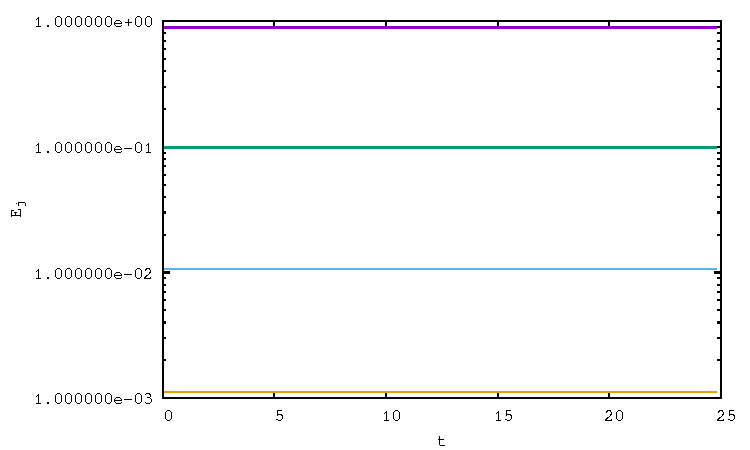
\includegraphics[width=\textwidth]{/Users/bradc/Research/Thesis/PhD/Chapter2/figs/paddedQPa2_00e-01_j200_lowjenergyevo}
		\caption{The evolution of the first four modes of the padded QP solution: {$j=0,1,2,3$} (purple, green, blue, orange).}
	\end{subfigure}
	\hfill
	%\begin{subfigure}[t]{0.45\textwidth}
	%	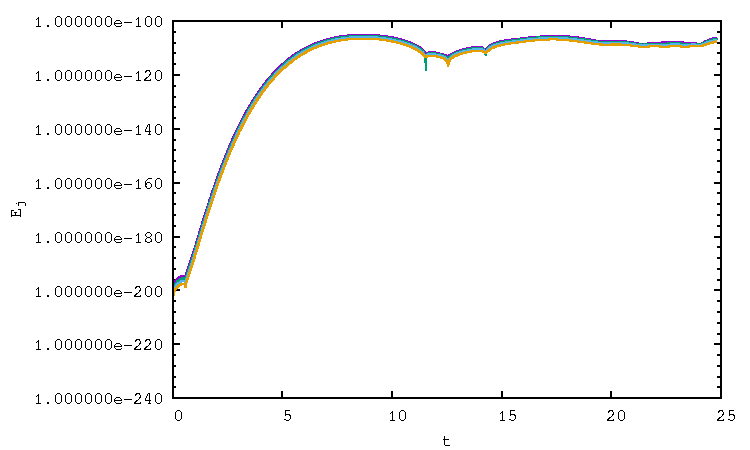
\includegraphics[width=\textwidth]{/Users/bradc/Research/Thesis/PhD/Chapter2/figs/paddedQPa2_00e-01_j200_highjenergyevo}
	%	\caption{The evolution of the last four modes: ${j = 196, 197, 198, 199}$ (purple, green, blue, orange).}
	%\end{subfigure}
	%\;
	\begin{subfigure}[t]{0.45\textwidth}
		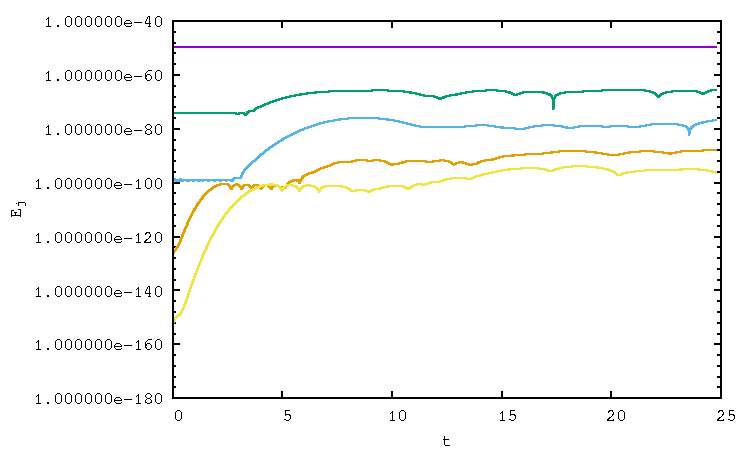
\includegraphics[width=\textwidth]{/Users/bradc/Research/Thesis/PhD/Chapter2/figs/paddedQPa2_00e-01_j200_energyevo}
		\caption{Comparing the evolution of a selection of modes: {$j= 50, 75, 100, 125, 150$} (purple, green, blue, orange, yellow).}
	\end{subfigure}
	\\
	\begin{subfigure}[t]{0.45\textwidth}
		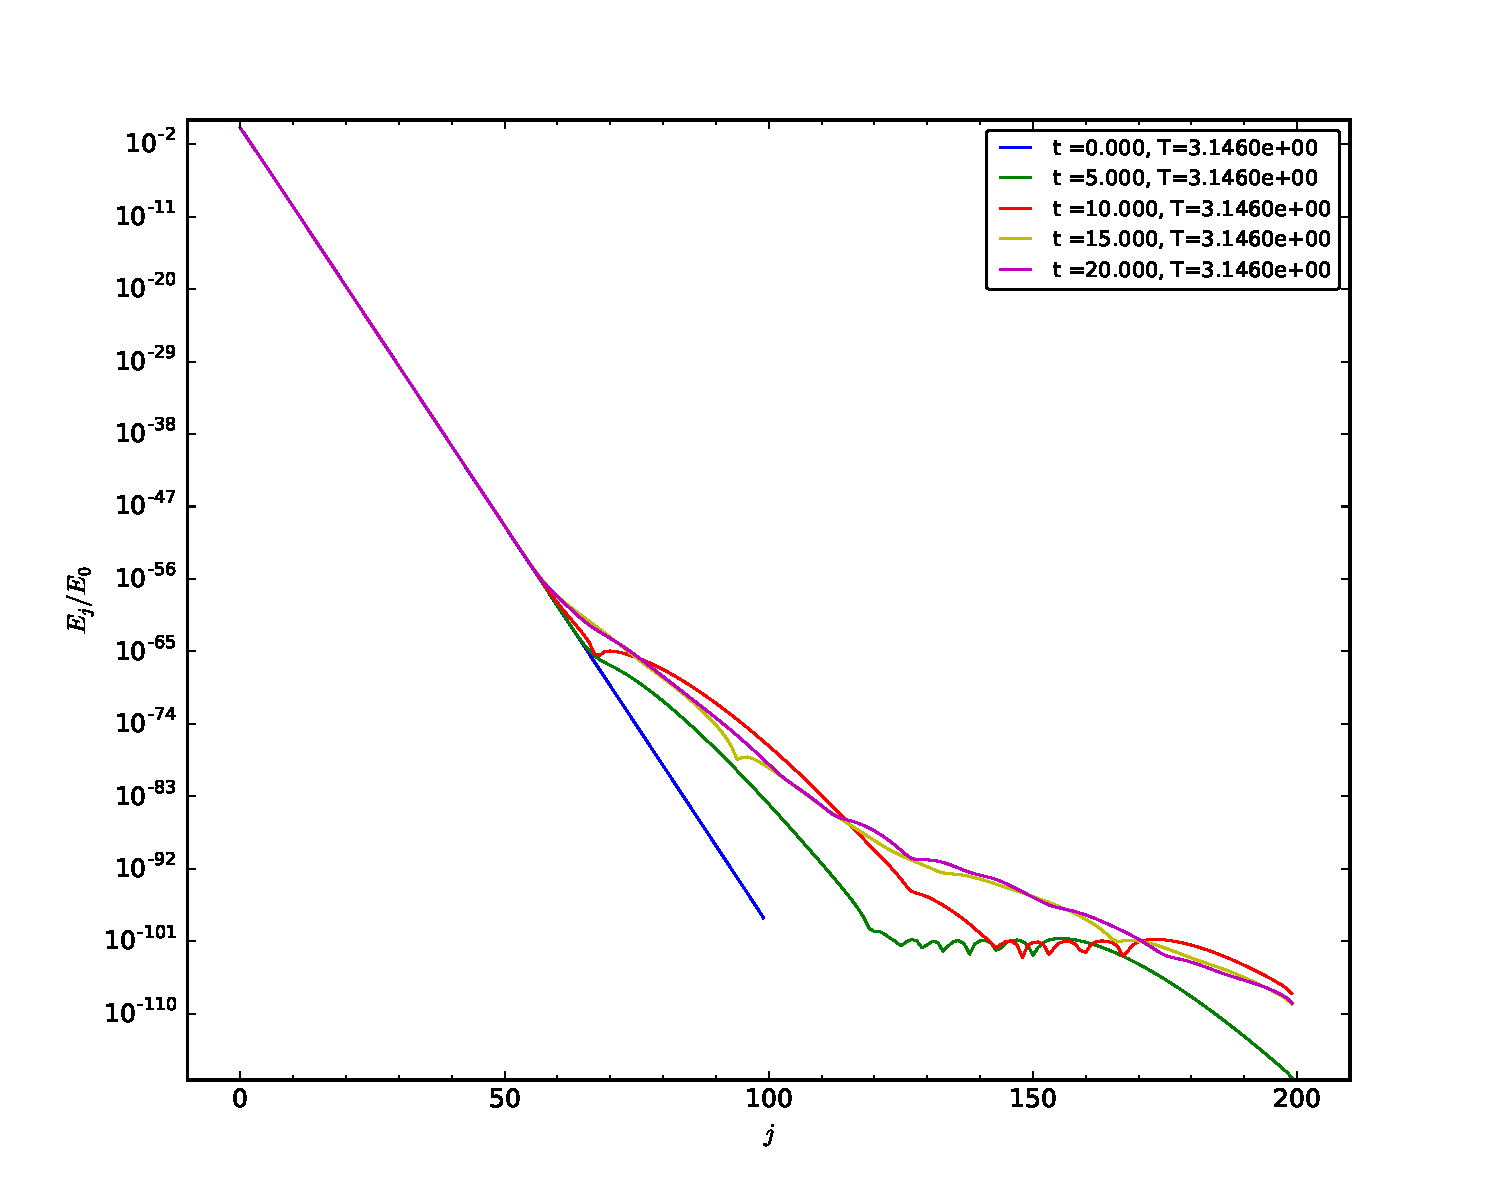
\includegraphics[width=\textwidth]{/Users/bradc/Research/Thesis/PhD/Chapter2/figs/paddedQPa2_00e-01_j200_spectrumevo}
		\caption{The total spectrum of the padded QP solution as a function of time.}
		\label{fig: paddedqp_fullspecevo}
	\end{subfigure}
	\:\:\:
	\begin{subfigure}[t]{0.45\textwidth}
		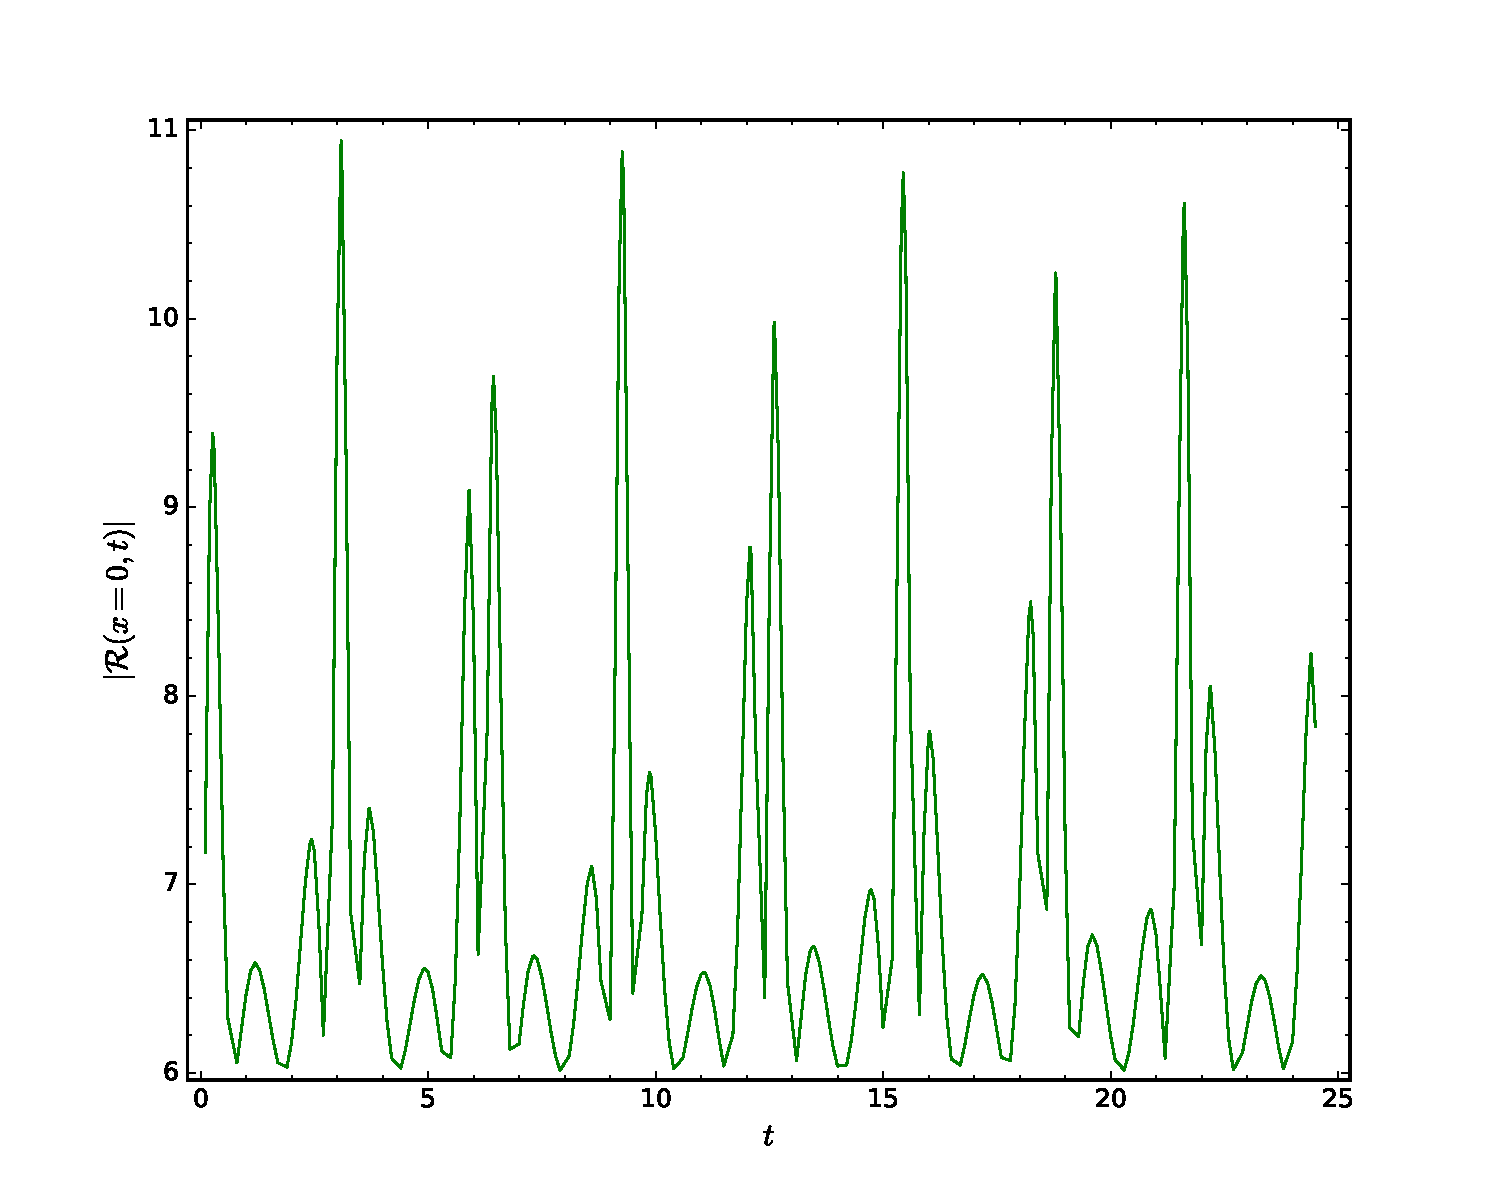
\includegraphics[width=\textwidth]{/Users/bradc/Research/Thesis/PhD/Chapter2/figs/Qpa2_00e-01padj200_ricci}
		\caption{The Ricci scalar at the origin as a function of time.}
		\label{fig: Qpa2_00e-01padj200_ricci}
	\end{subfigure}
	\caption[The evolution of a padded QP solution]{The evolution of the padded QP solution for $\alpha_1 =0.2$ and $\jm = 200$, with amplitude $\epsilon=0.27$ over $t \in [0, 25]$.}
	\label{fig:paddedqpevo}
\end{figure}

%\begin{figure}[ht]
%	\centering
%	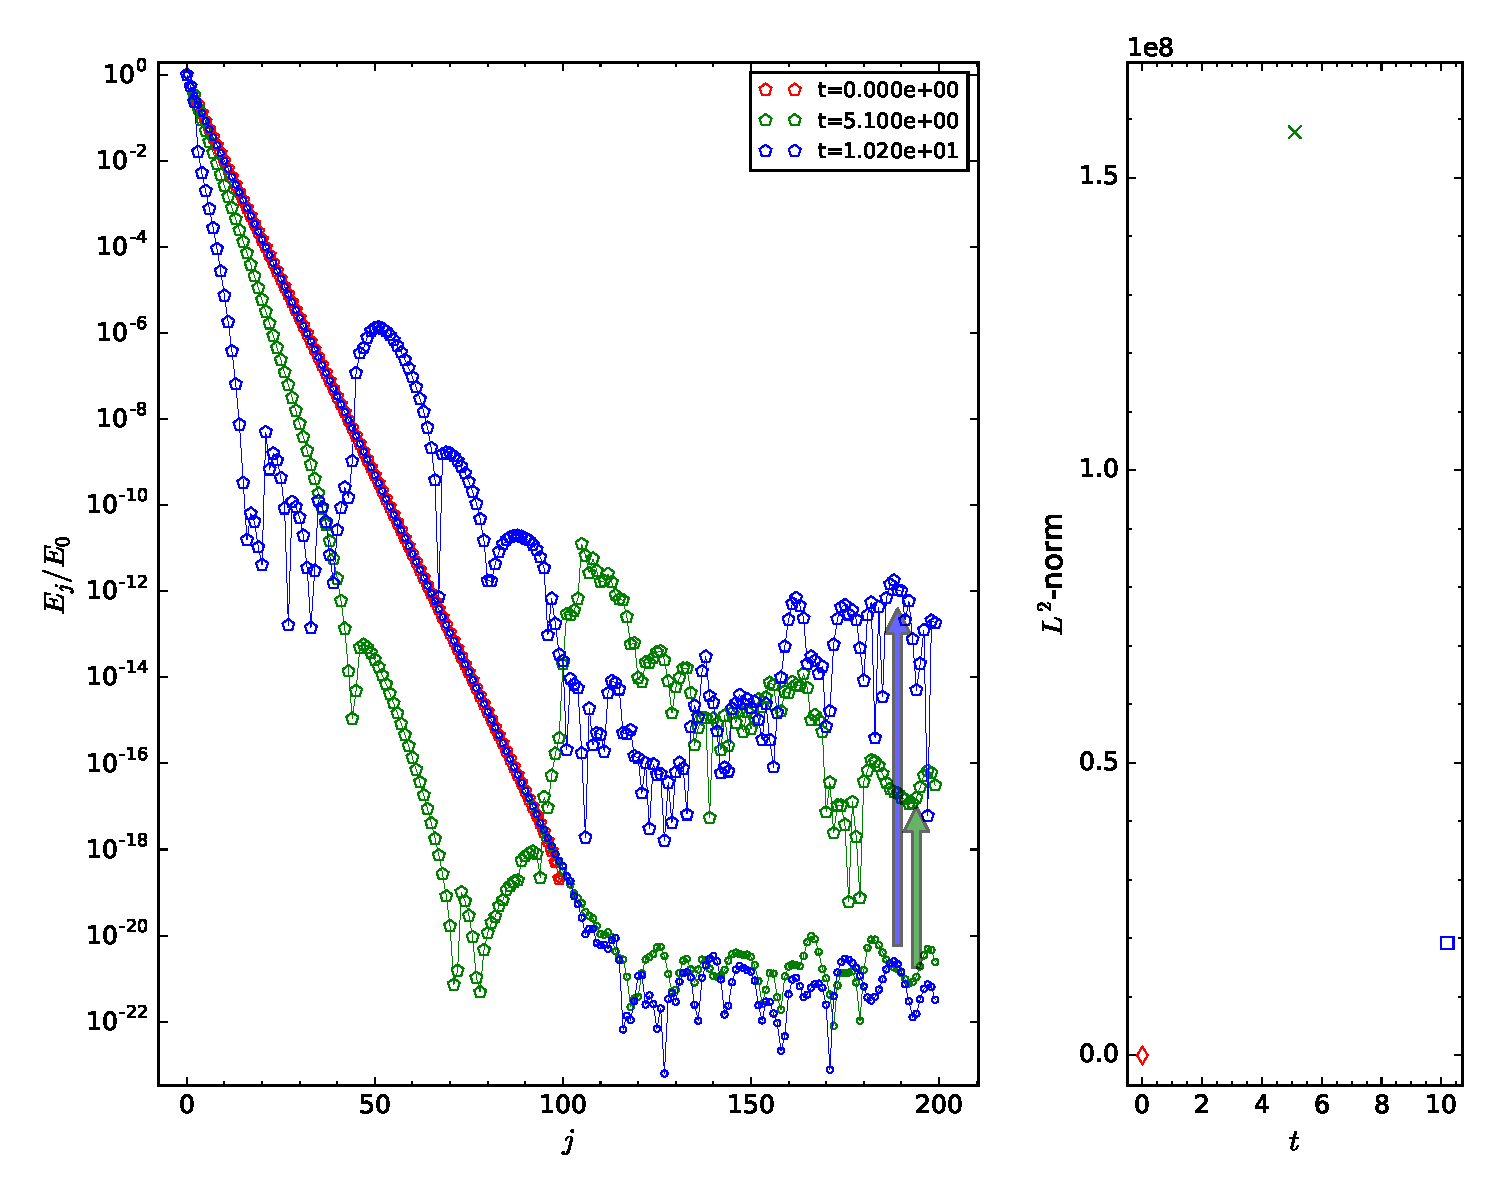
\includegraphics[width=0.75\textwidth]{/Users/bradc/Research/Thesis/PhD/Chapter2/figs/QPa4_40e-01padj200_evolutionprojection}
%	\caption[Evolving a padded QP solution]{A low temperature QP solution is padded with zeros out to $\jm = 200$ and evolved in time with $\epsilon=0.1$. Intermediate solutions are projected back to the QP surface at $t \simeq 0.0, 5.1, 10.2 $ (red diamond, green cross, blue square)}
%	\label{fig: QPa4_40e-01padj200_evolutionprojection}
%\end{figure}

%\begin{figure}[ht]
%	\begin{subfigure}[t]{0.45\textwidth}
%		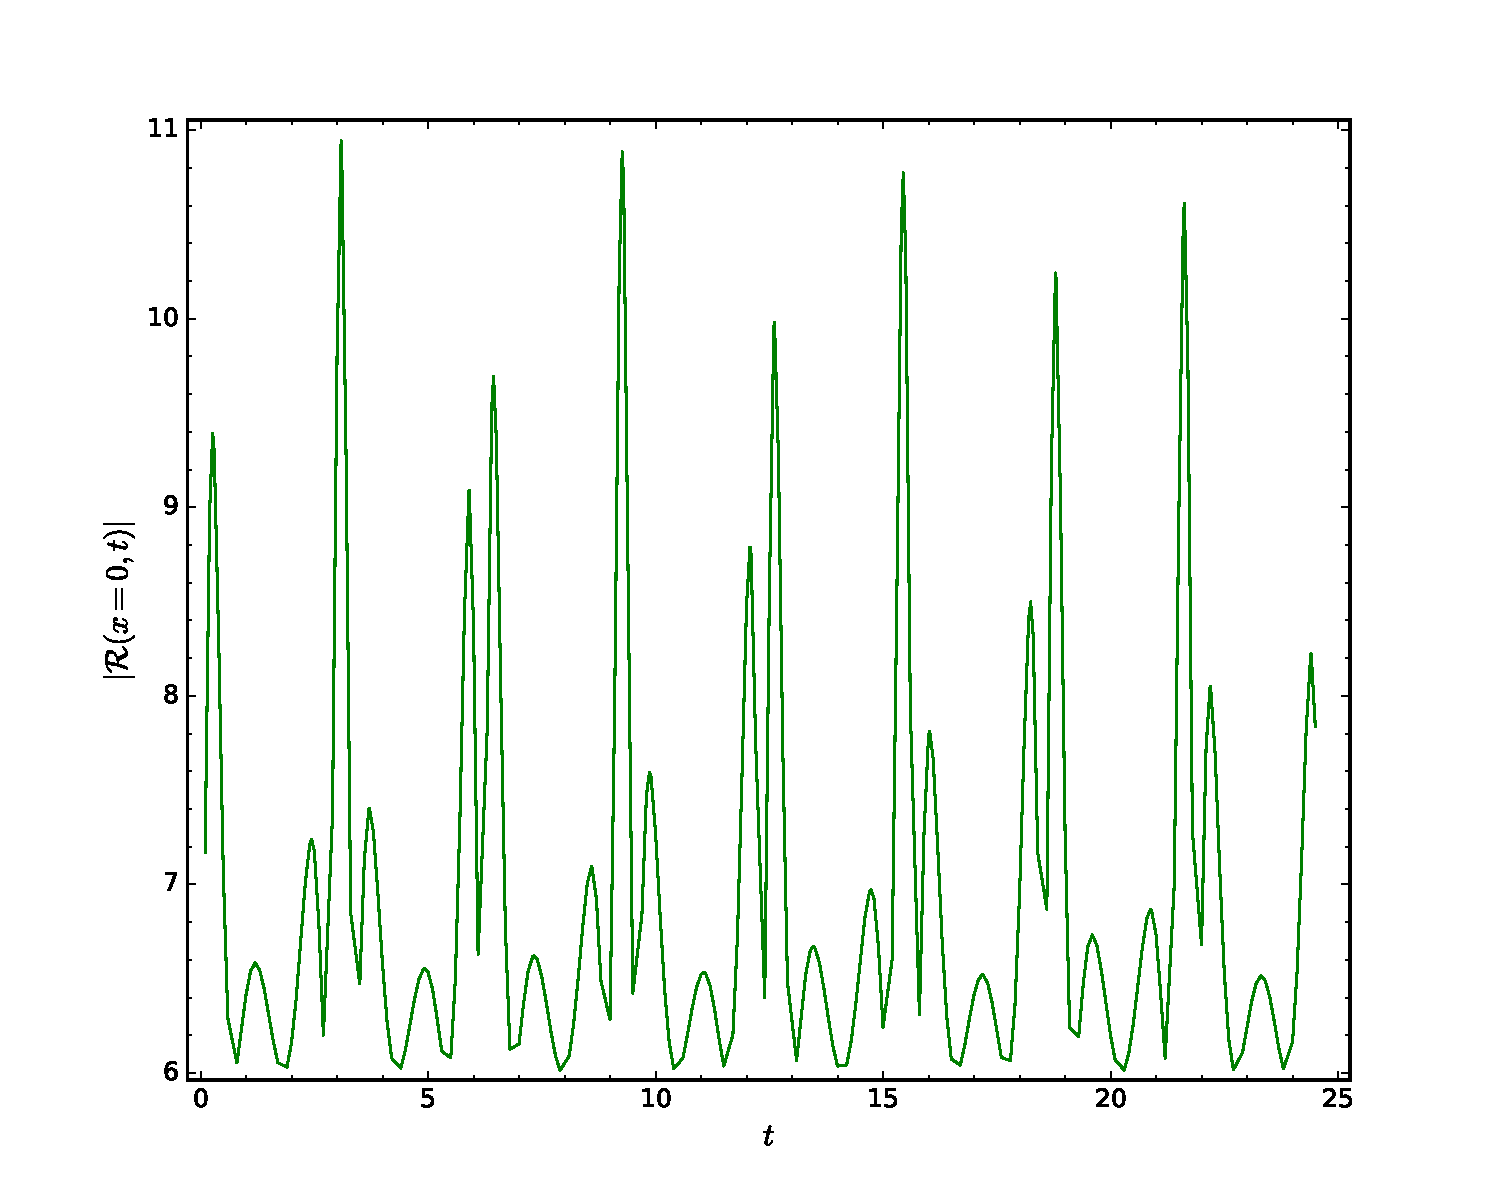
\includegraphics[width=\textwidth]{/Users/bradc/Research/Thesis/PhD/Chapter2/figs/Qpa2_00e-01padj200_ricci}
%		\caption{The Ricci scalar at the origin as a function of time.}
%		\label{fig: Qpa2_00e-01padj200_ricci}
%	\end{subfigure}
%	\;
%	\begin{subfigure}[t]{0.45\textwidth}
%		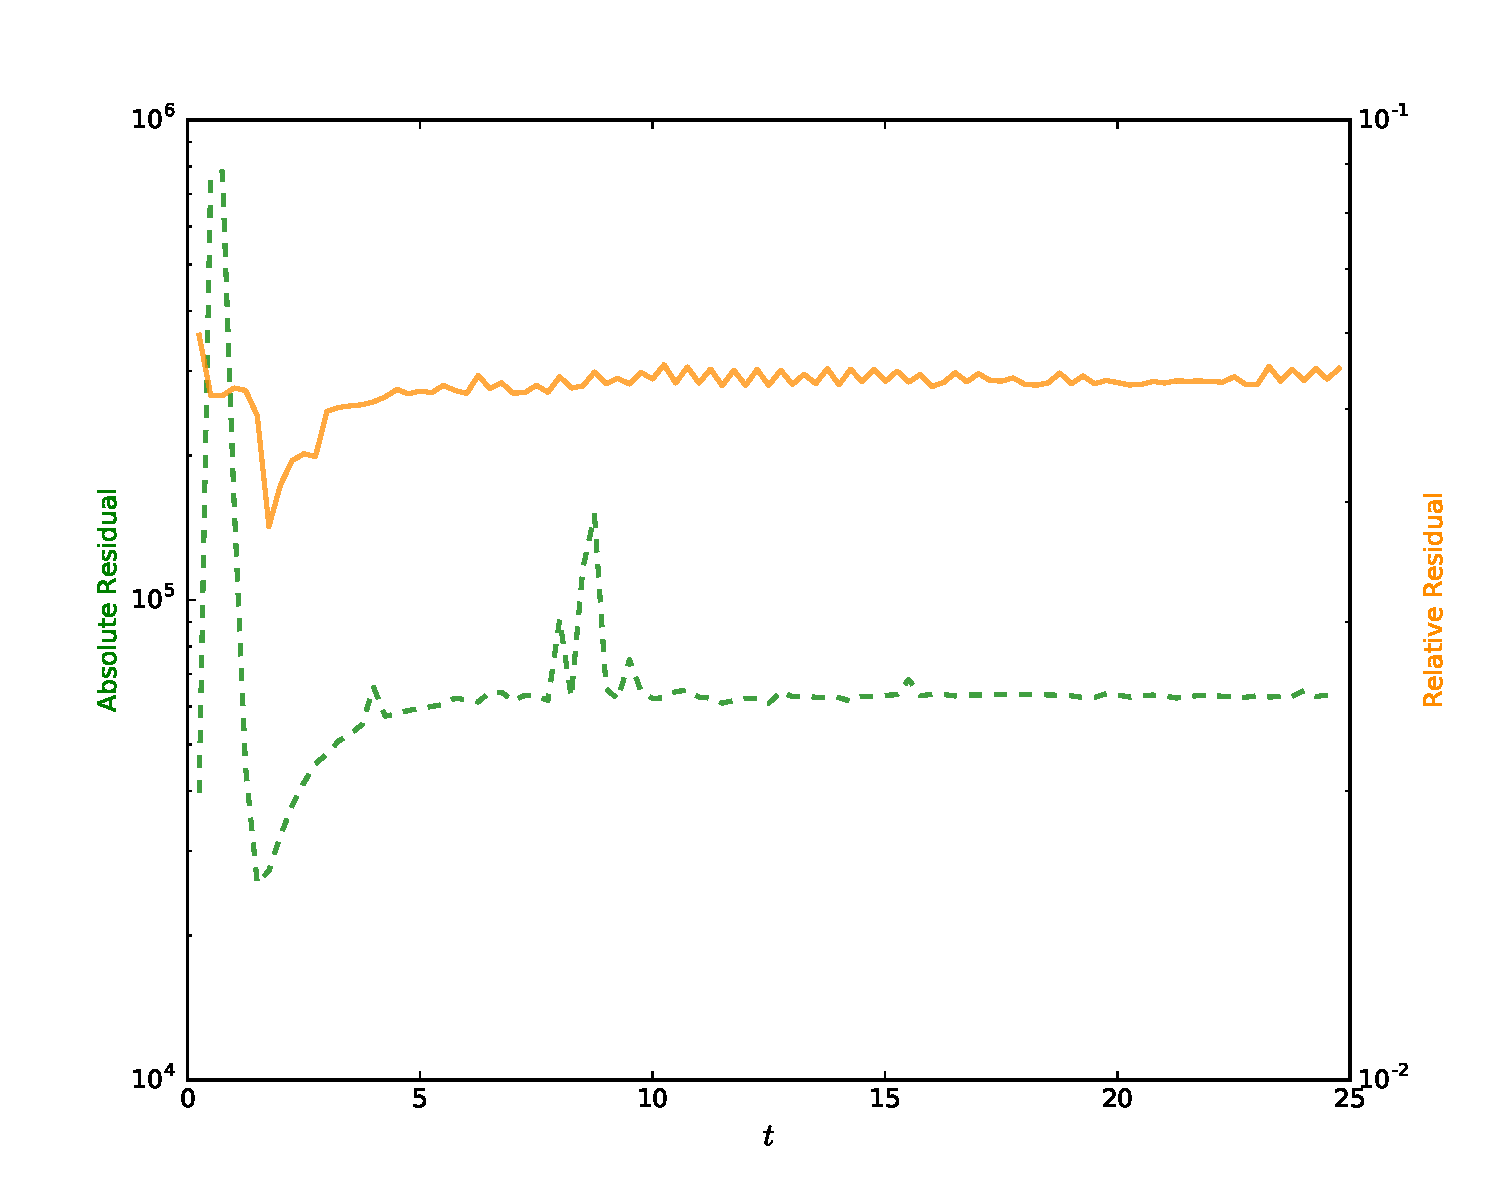
\includegraphics[width=\textwidth]{/Users/bradc/Research/Thesis/PhD/Chapter2/figs/Qp2_00e-01padj200_resids}
%		\caption{The residuals of the QP equation during the evolution of the padded QP solution.}
%		\label{fig: Qp2_00e-01padj200_resids}
%	\end{subfigure}
%	\caption[Stability indicators for a padded QP solution]{Measures of stability for an $\alpha_1 = 0.2$, $\jm = 100$ QP solution that has been padded with zeros to $\jm = 200$.}
%	\label{fig:paddedqpstab}
%	\caption{}
%	\end{figure}

%\begin{figure}[ht]
%	\centering
%	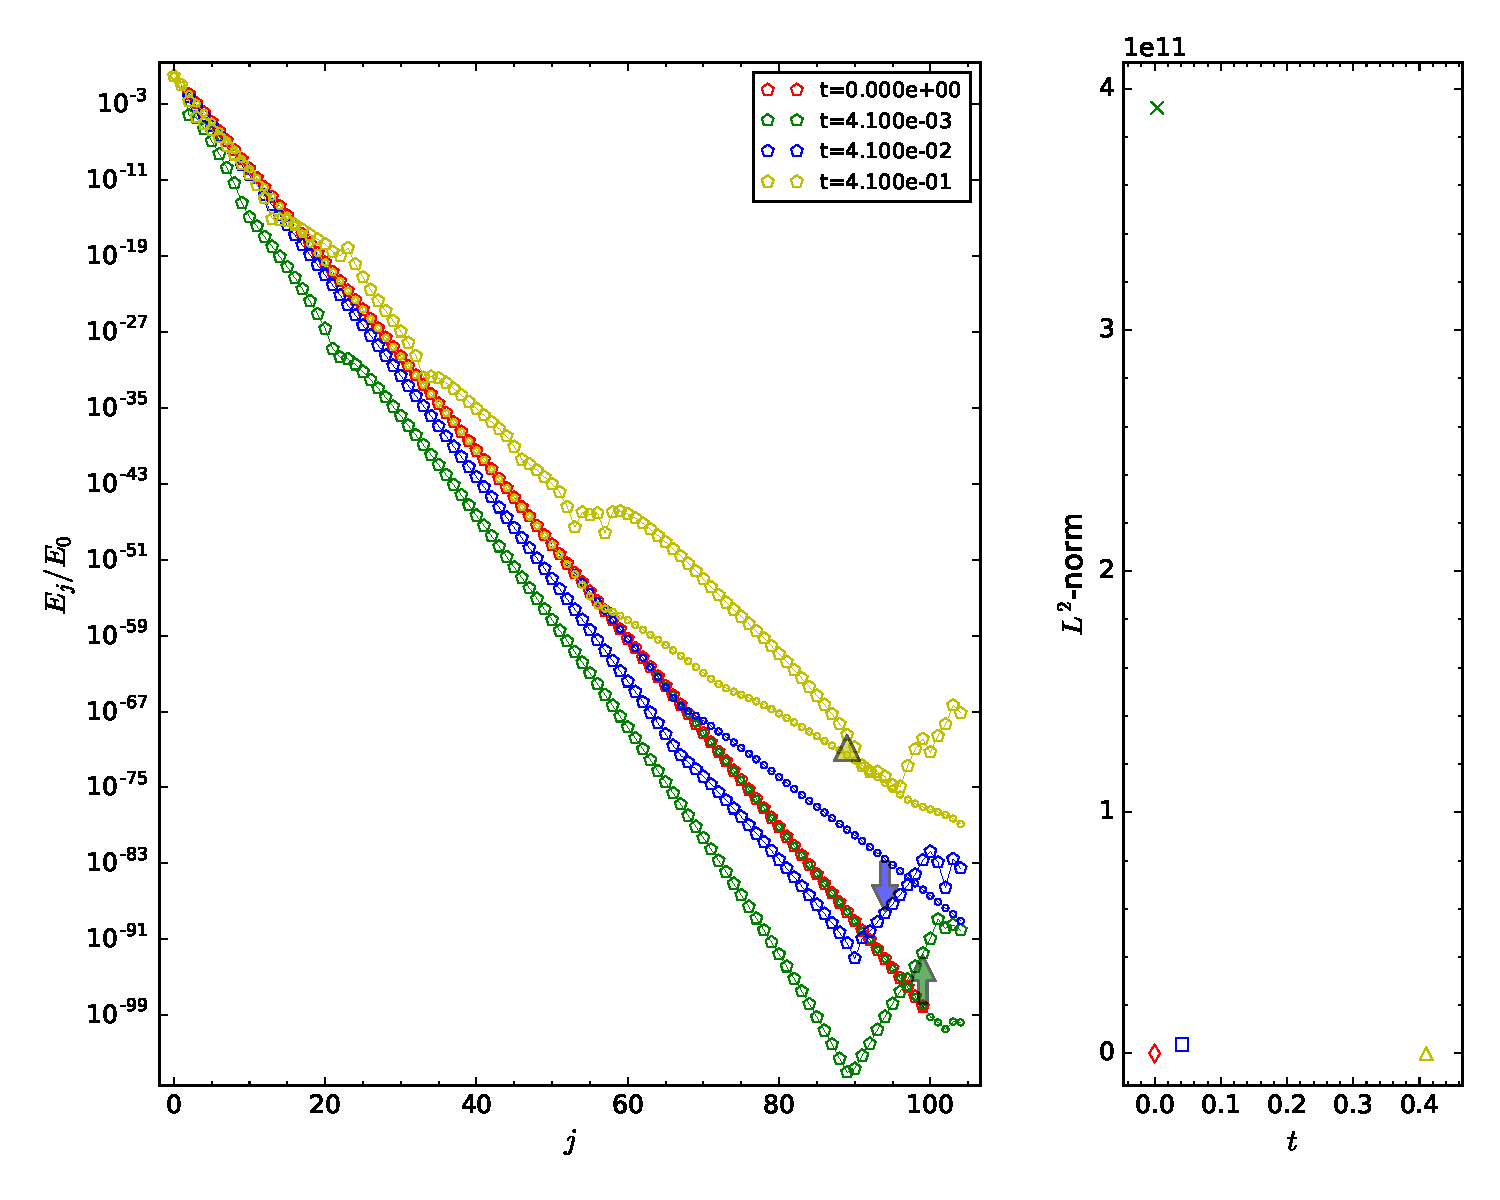
\includegraphics[width=0.75\textwidth]{/Users/bradc/Research/Thesis/PhD/Chapter2/figs/Qpa2_00e-01padj105_evolutionprojection}
%	\caption[Spectra during evolution of a padded QP solution are used as seeds to project back to the QP surface]{{\it Left}: Normalized spectra for a $\jm = 100$, QP solution that has been padded with five extra modes, then evolved in time. Intermediate spectra are used as seeds for projecting back to the QP surface at times $\tau \simeq 4.1 \times 10^{-3}, 4.1 \times 10^{-2}, 4.1 \times 10^{-1}$ (green, blue, yellow). Arrows are oriented from seed spectra to best fit spectra. {\it Right:} Corresponding $L^2$-norms of the error for each solution.}
%	\label{fig: Qpa2_00e-01padj105_evolutionprojection}
%\end{figure}

%%%%%%%%%%%%%%%%%%%%%%%%%%%%%%%%%%%%%%%%%

\subsection{High-Temperature QP Data}

We now apply the same amplitude-phase evolution procedure to higher temperature QP data. First, we consider a QP solution with $\jm = 100$ and $T \simeq 5.4$. Such a solution was demonstrated in figure~\ref{fig: const T perturbs} to be robust as $\jm$ increased. In figure~\ref{fig: HighTa4_072e-01j100T5_3921e+00_highjevo} we show  the fractional energy per mode during evolution. Because of the initial profile of solutions with these temperatures, there is a much higher fraction of the total energy in the higher modes; therefore, the accumulation of numerical errors that were present in low-temperature solutions are not as significant. Close inspection of figure~\ref{fig: HighTa4_072e-01j100T5_3921e+00_highjevo}, shows small oscillations in the fractional energy of the high frequency components of the scalar field. However, these oscillations are not sufficient to produce a qualitative change in the full energy spectrum, as shown in the left pane of figure~\ref{fig:HighTa4_072e-01j100T5_3921e+00_evo}. Examination of the absolute value of the scalar curvature at the origin in the right pane of figure~\ref{fig:HighTa4_072e-01j100T5_3921e+00_evo} shows that the large initial value of $| \mc R |$ oscillates rapidly during evolution. Since the TTF description is inherently stable, the curvature will never become infinite; however, large values of curvature with rapid oscillations are good indicators of instability. It would be interesting to use such a solution as initial data for evolution in the fully nonlinear system to test if stability is maintained over the perturbative timescale. 
\vspace{0.1in}
\begin{figure}[H]
	\centering
	\begin{subfigure}[t]{0.48\textwidth}
		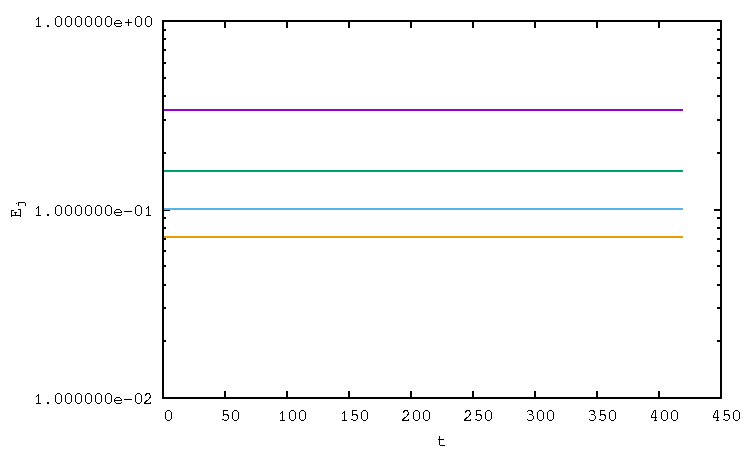
\includegraphics[width=\textwidth]{/Users/bradc/Research/Thesis/PhD/Chapter2/figs/HighTa4_072e-01j100T5_3921e+00_lowjevo}
		\label{}
	\end{subfigure}
	\hfill
	\begin{subfigure}[t]{0.48\textwidth}
		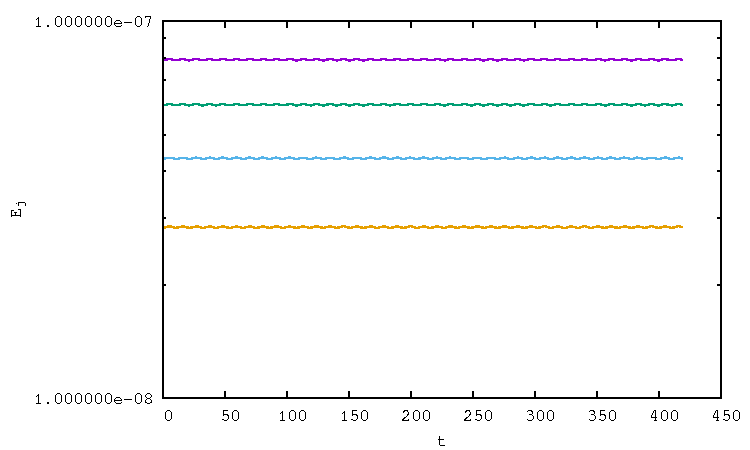
\includegraphics[width=\textwidth]{/Users/bradc/Research/Thesis/PhD/Chapter2/figs/HighTa4_072e-01j100T5_3921e+00_highjevo}
		\label{}
	\end{subfigure}
	\caption[Examining the energy per mode during the evolution of a $T \simeq 5.4$ QP solution]{Examining the energy per mode during the evolution of a $T \simeq 5.4$ QP solution with ${\epsilon = 0.1}$ over ${t \in [0, 425]}$. $E_j$ for ${j = 0, 1, 2, 3}$ (purple, green, blue, orange) is on the left,  $E_j$ for ${j = 96, 97, 98, 99}$ (purple, green, blue, orange) is on the right.}
	\label{fig: HighTa4_072e-01j100T5_3921e+00_highjevo}
\end{figure}
	
\begin{figure}[H]
	\begin{subfigure}[t]{0.48\textwidth}
		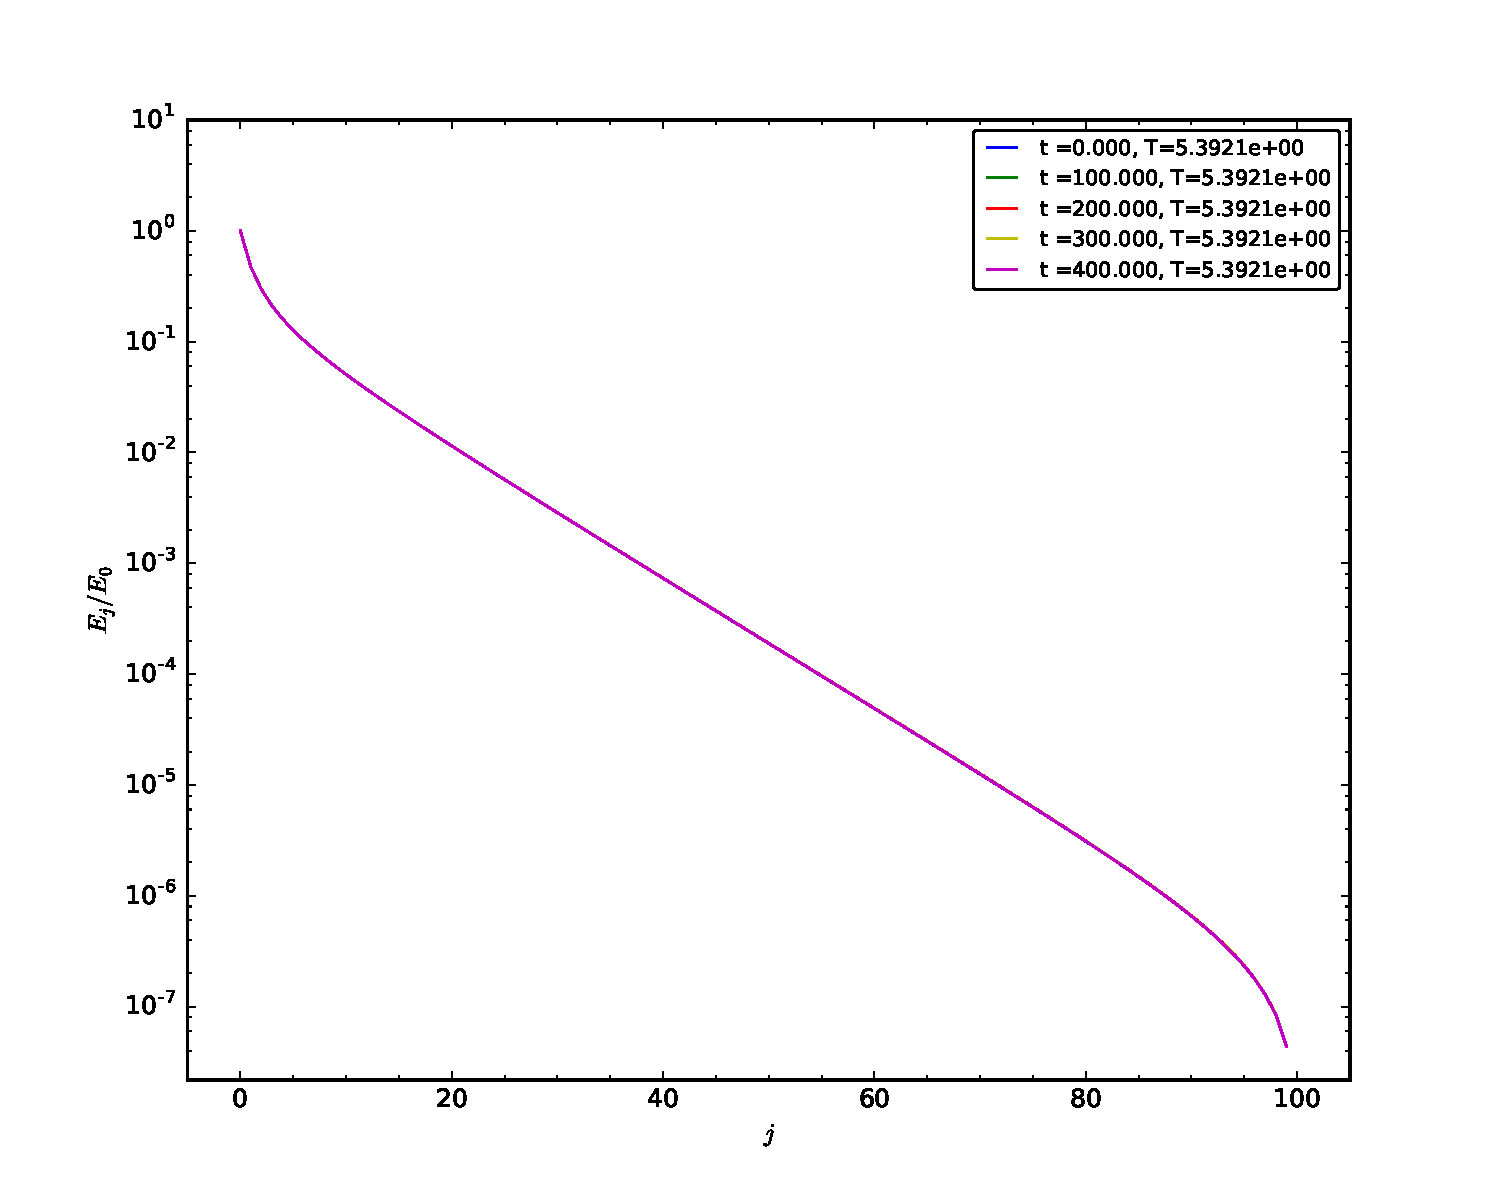
\includegraphics[width=\textwidth]{/Users/bradc/Research/Thesis/PhD/Chapter2/figs/HighTa4_072e-01j100T5_3921e+00_spectrumevo}
		\label{fig: HighTa4_072e-01j100T5_3921e+00_spectrumevo}
	\end{subfigure}
	\:
	\begin{subfigure}[t]{0.48\textwidth}
		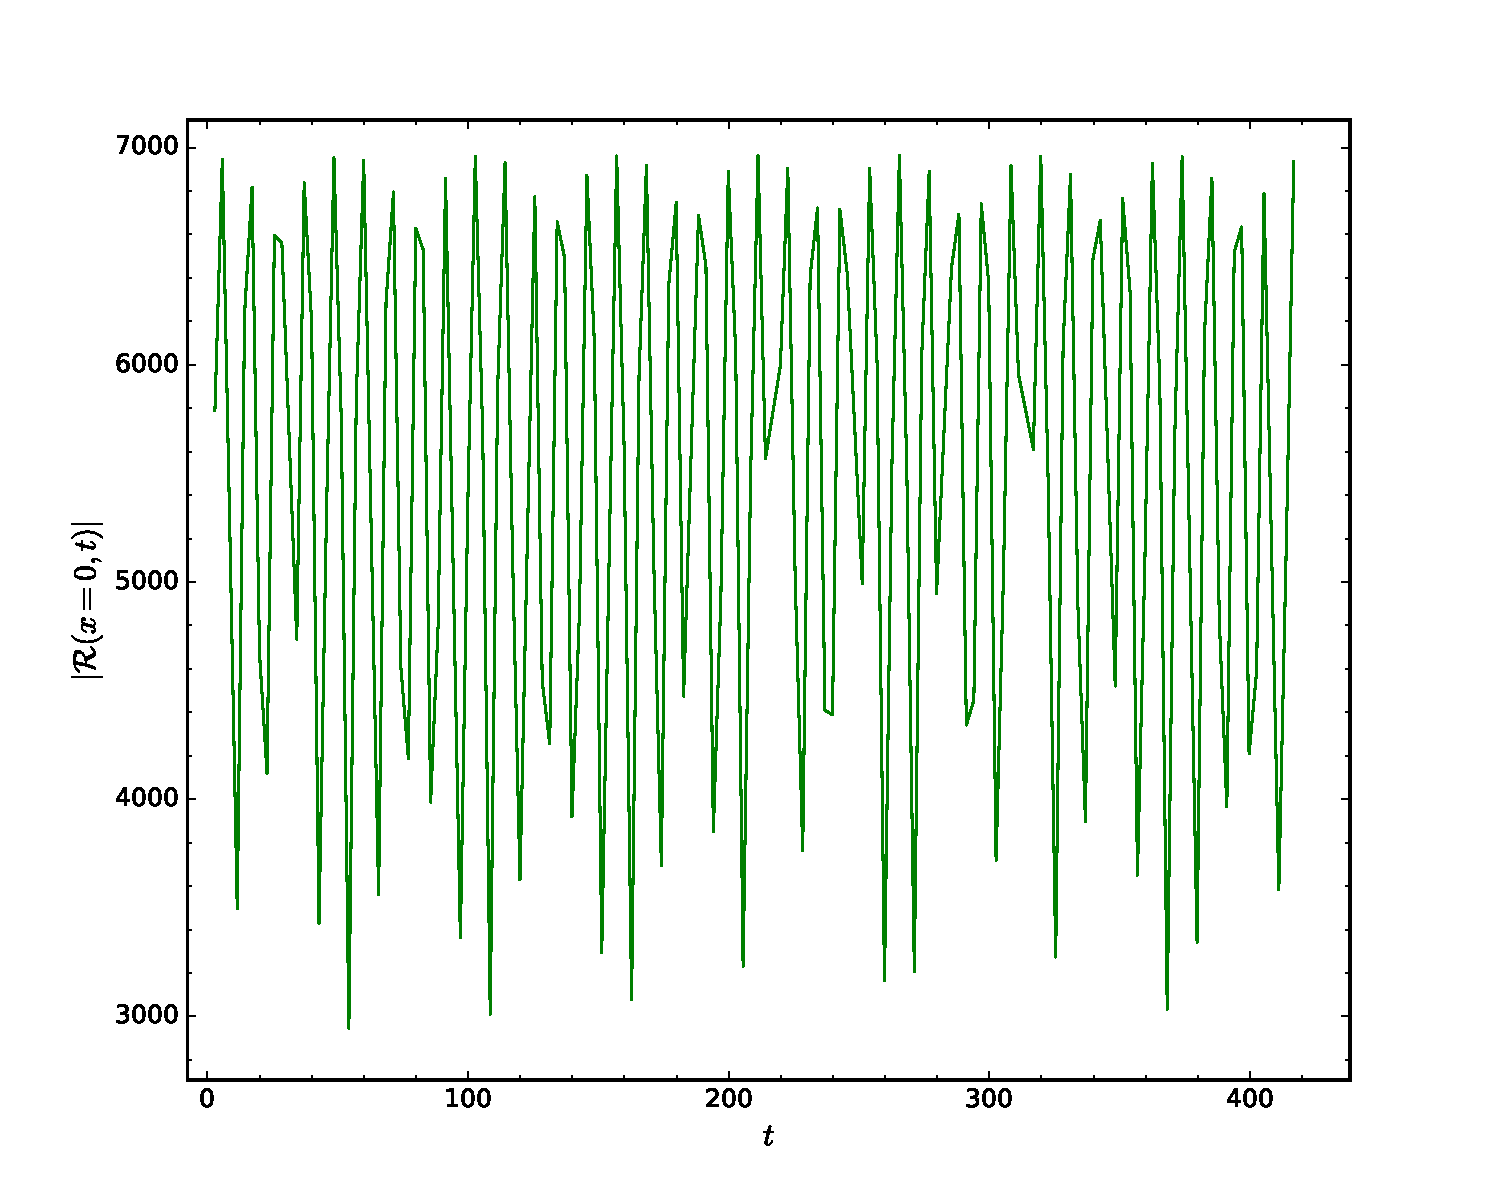
\includegraphics[width=\textwidth]{/Users/bradc/Research/Thesis/PhD/Chapter2/figs/HighTa4_072e-01j100T5_3921e+00Ricci}
		\label{fig: HighTa4_072e-01j100T5_3921e+00Ricci}
	\end{subfigure}
	\caption[Evolution of the energy spectrum and Ricci scalar for a $T \simeq 5.4$ QP solution]{The evolution of the energy spectrum (left) and upper envelope of the Ricci scalar (right) for a $T \simeq 5.4$ QP solution with $\epsilon = 0.1$ over $t \in [0, 425]$.}
	\label{fig:HighTa4_072e-01j100T5_3921e+00_evo}	
\end{figure}

\begin{figure}[h]
	\centering
%	\begin{subfigure}[t]{0.45\textwidth}
%		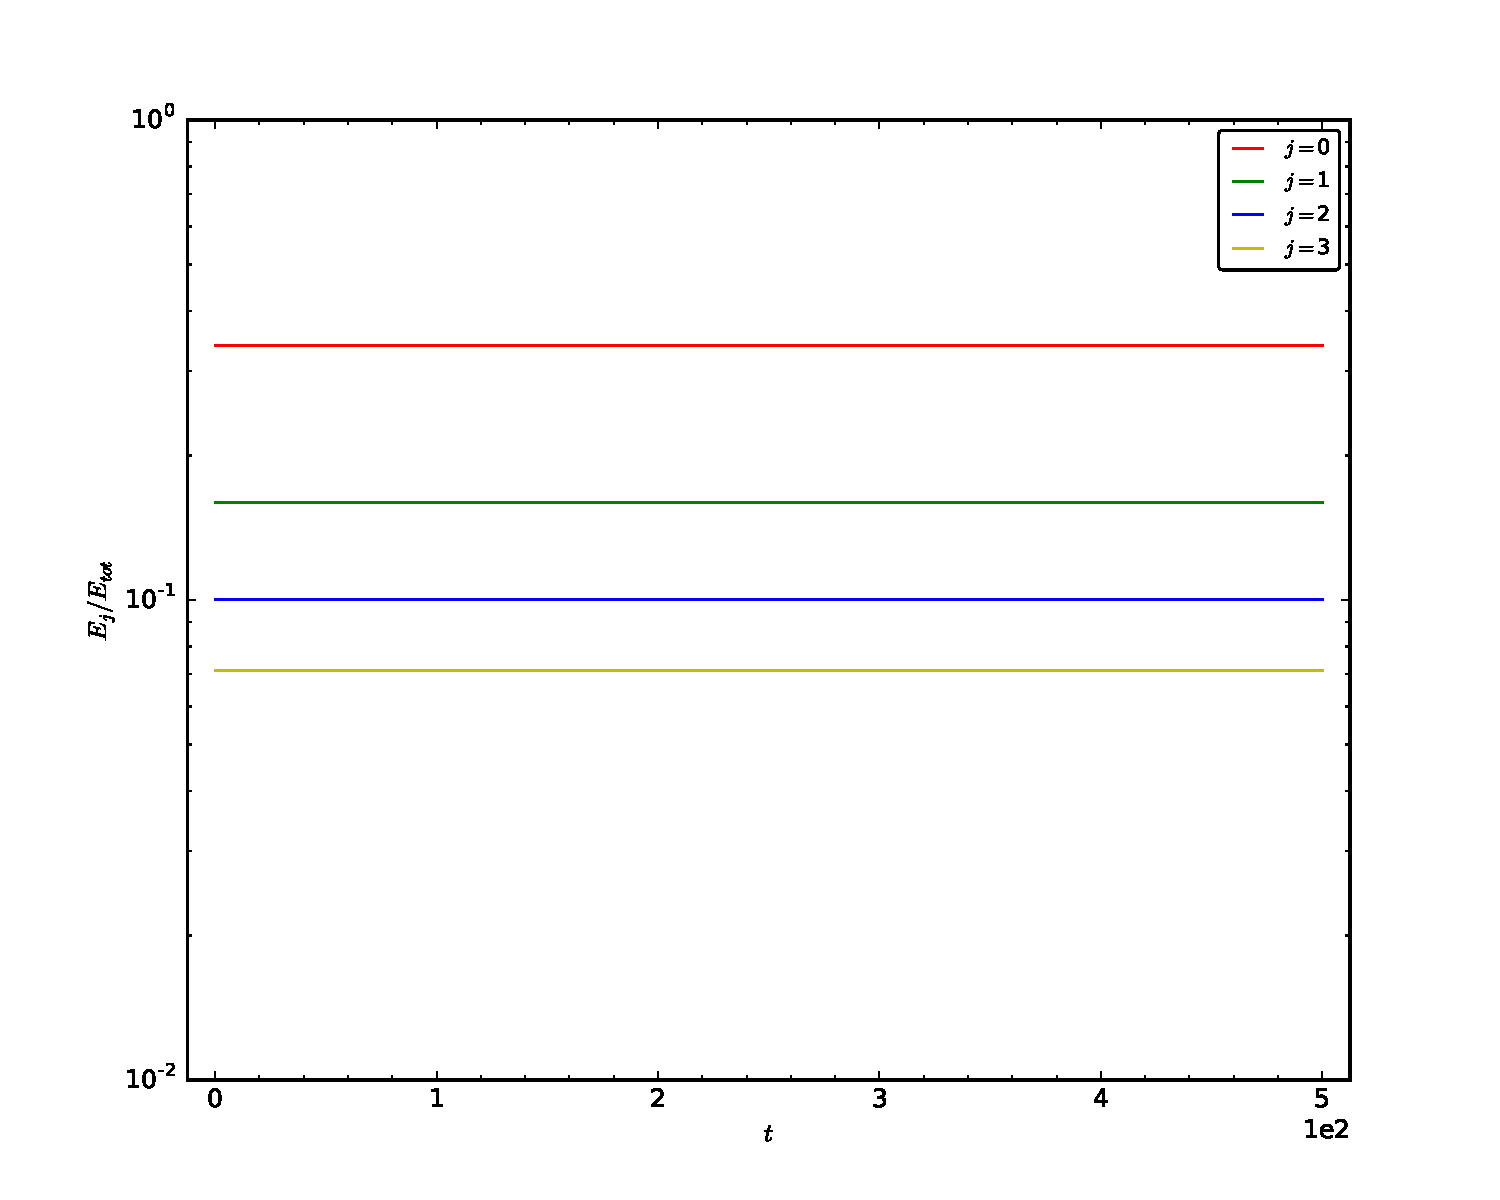
\includegraphics[width=\textwidth]{/Users/bradc/Research/Thesis/PhD/Chapter2/figs/HighTa4_072e-01padj200T5_3921e+00_lowjevo}
%	\end{subfigure}
%	\;
	\begin{subfigure}[t]{0.45\textwidth}
		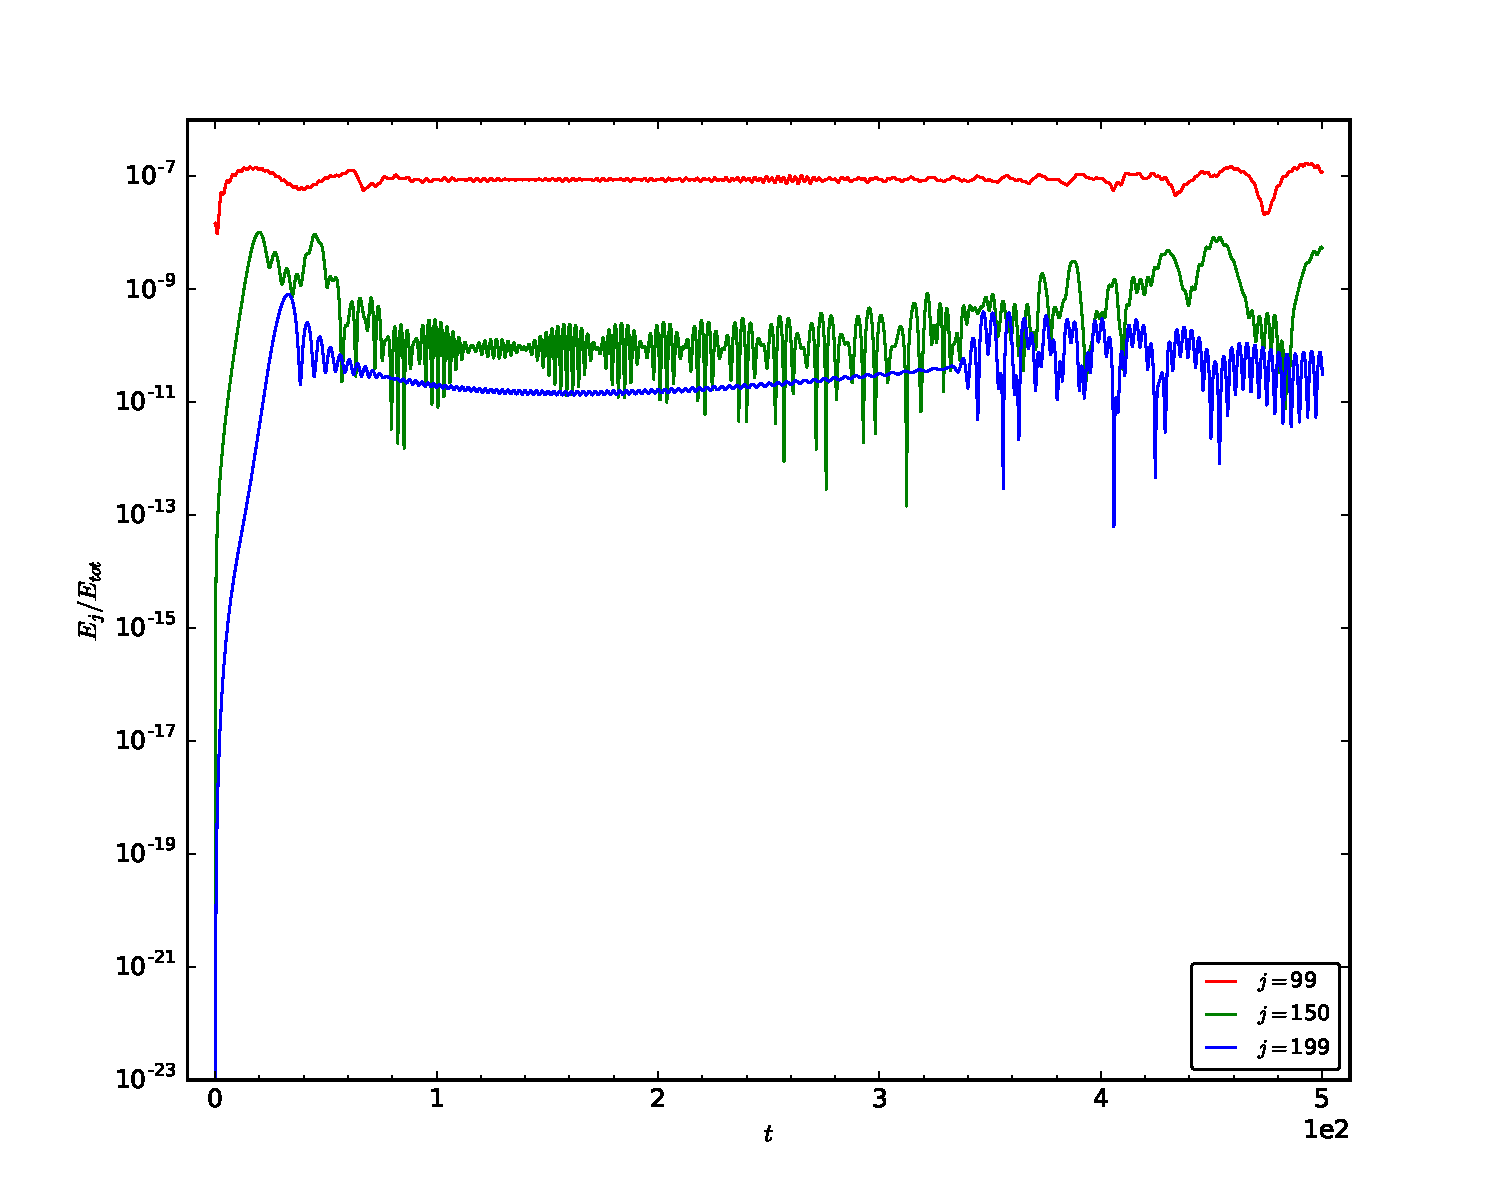
\includegraphics[width=\textwidth]{/Users/bradc/Research/Thesis/PhD/Chapter2/figs/HighTa4_072e-01padj200T5_3921e+00_evo}
	\end{subfigure}
	\;
	\begin{subfigure}[t]{0.45\textwidth}
		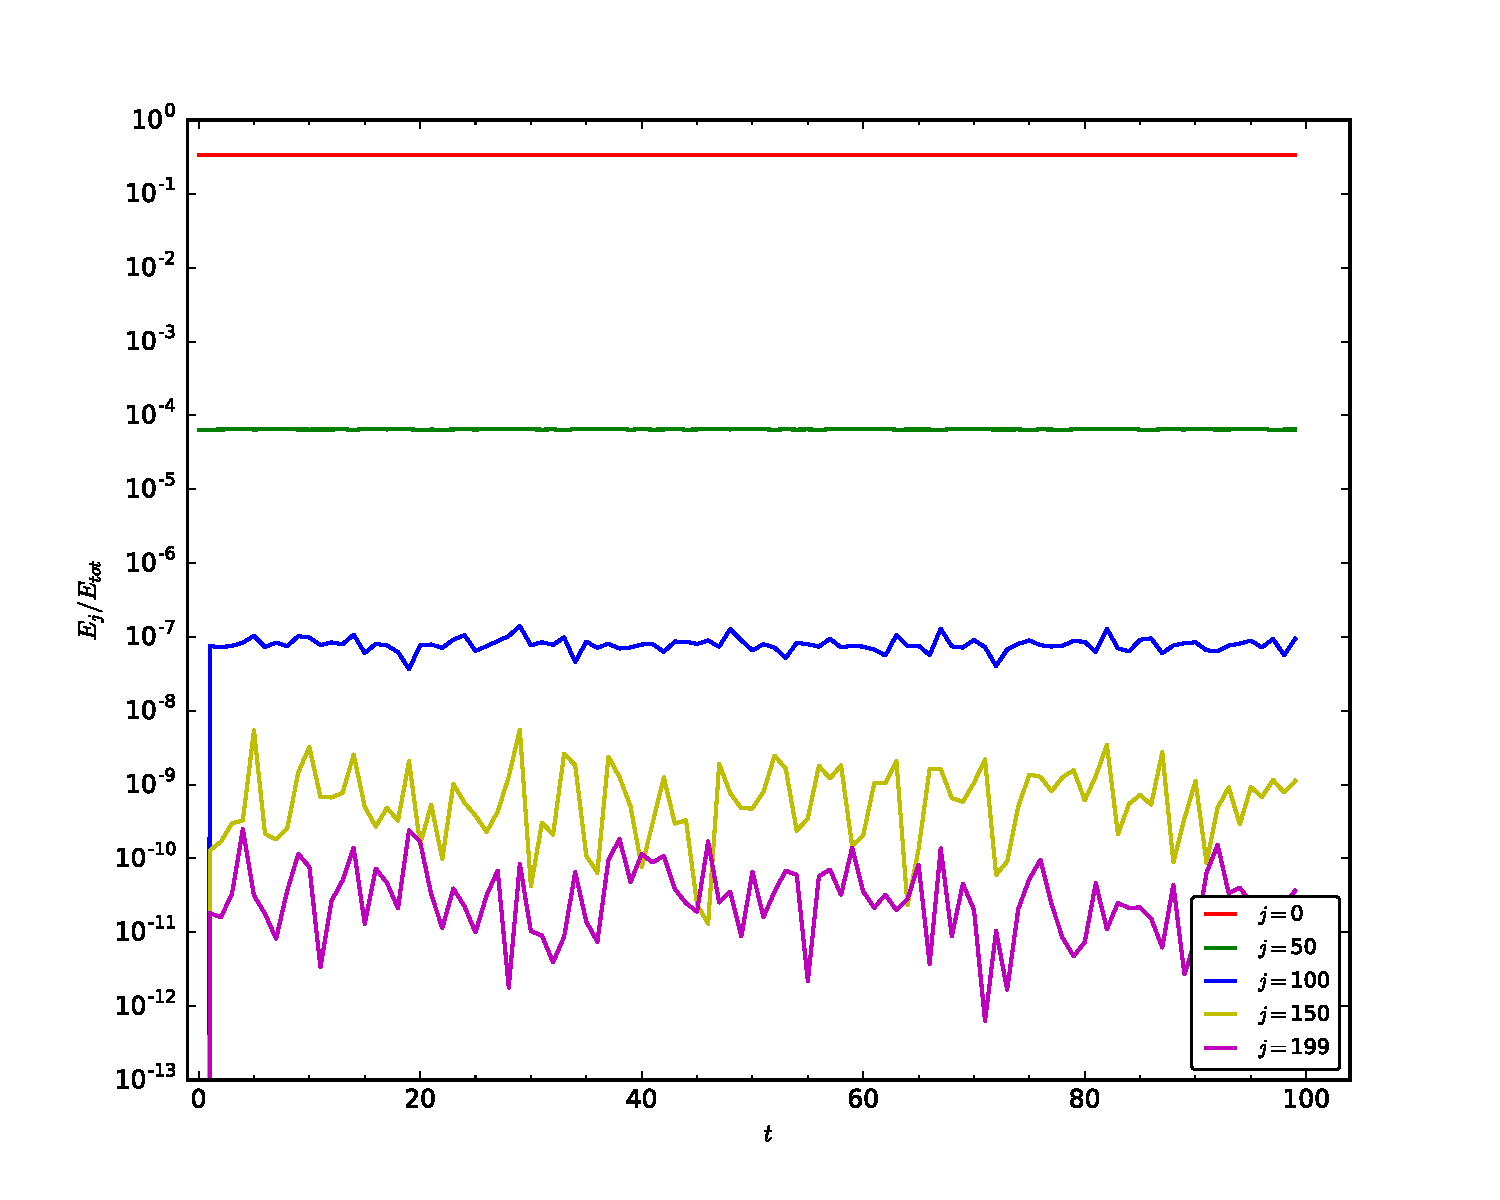
\includegraphics[width=\textwidth]{/Users/bradc/Research/Thesis/PhD/Chapter2/figs/HighTa4_072e-01padj200T5_3921e+00_spectrum}
	\end{subfigure}
	\caption[Evolution of the spectrum of a $T \simeq 5.4$ QP solution that has been padded with $100$ modes]{A $T \simeq 5.4$ QP solution shown in figure~\ref{fig:HighTa4_072e-01j100T5_3921e+00_evo} is padded with 100 extra modes and evolved with $\epsilon = 0.1$ over $t \in [0, 100]$}
	\label{fig: HighTa4_072e-01padj200T5_3921e+00_evo}
\end{figure}

\begin{figure}[ht]
	\centering
	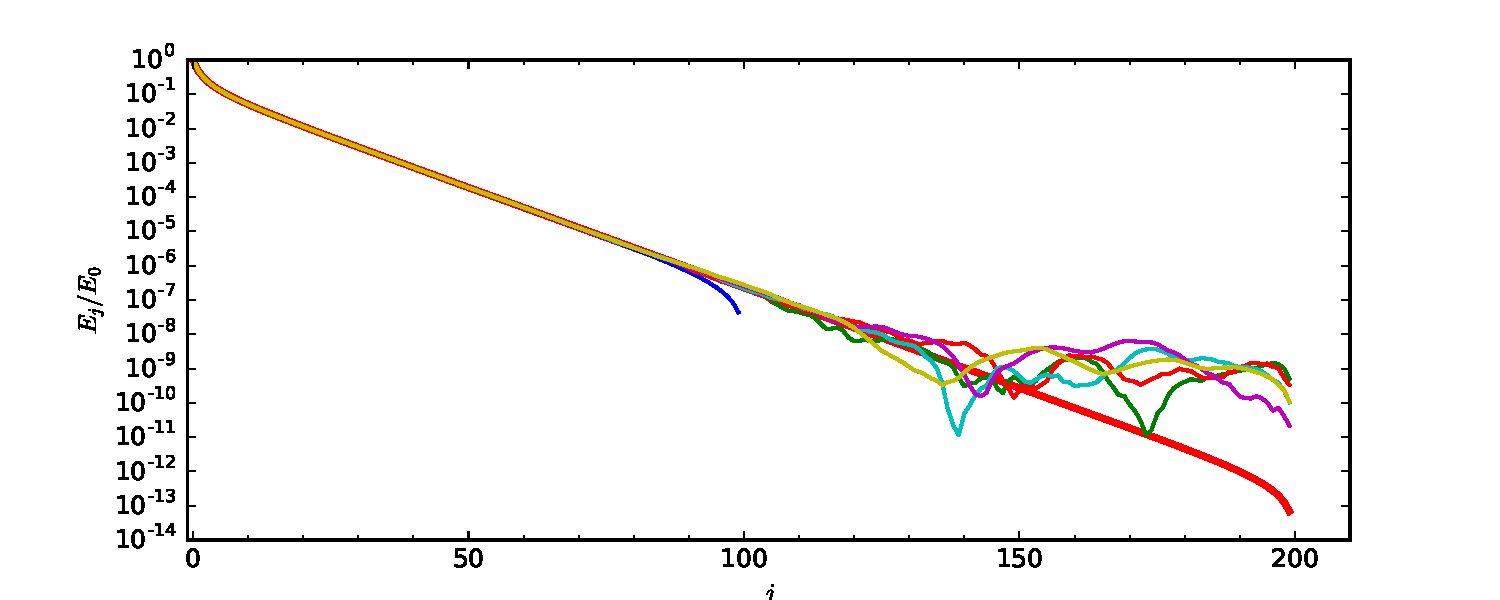
\includegraphics[width=0.75\textwidth]{/Users/bradc/Research/Thesis/PhD/Chapter2/figs/HighTa4_072e-01spec_vs_padv2}
	\caption[Comparison between a attracor solution with $j_{max} = 200$ and the evolution of a $j_{max} = 100$, $T \simeq 5.4$ solution that has been padded by $100$ modes]{Overlay of the known $T \simeq 5.4$ solution for $\jm = 200$ (thick red line) with the spectra in figure~\ref{fig: HighTa4_072e-01padj200T5_3921e+00_evo}.}
	\label{fig: HighTa4_072e-01spec_vs_pad}
\end{figure}

As in the case of low-temperature QP solutions, we wish to expand the space of possible solutions by padding high temperature solutions with extra modes that are initially set to zero. To do so, we consider padding a $T \simeq 5.4$ QP solution from $\jm = 100$ to $\jm = 200$ with $\alpha_j = 0$ for $j > 99$. Figure~\ref{fig: HighTa4_072e-01padj200T5_3921e+00_evo} demonstrates that after evolving in time there are indications of large scale energy transfer amongst modes with higher frequencies. Interestingly, the magnitude and oscillation frequency of the Ricci scalar at the origin is significantly decreased compared to the $\jm = 100$, $T \simeq 5.4$ solution. When compared against the known solution of the same temperature when $\jm = 200$, figure~\ref{fig: HighTa4_072e-01spec_vs_pad} indicates that the padded solution may not approach the known QP solution and instead may have produced a distinct, isothermal, but non quasi-periodic, solution.

%\begin{figure}[ht]
%	\centering
%	\begin{subfigure}[t]{0.45\textwidth}
%		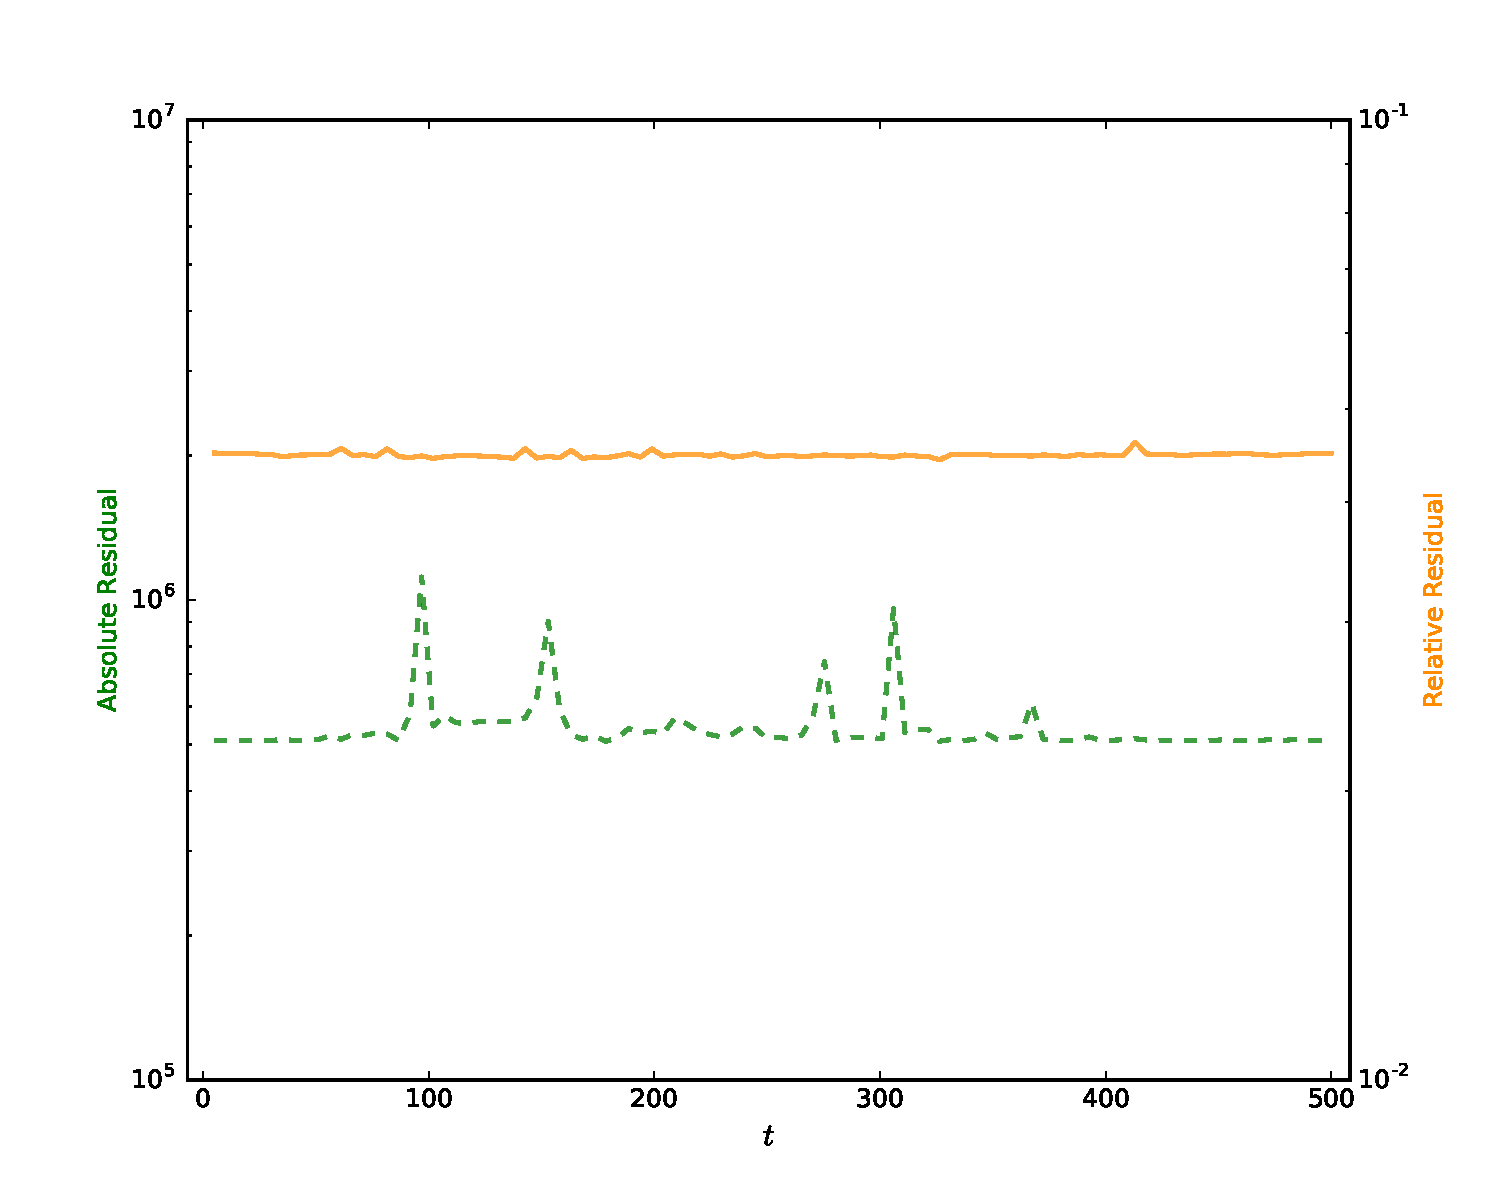
\includegraphics[width=\textwidth]{/Users/bradc/Research/Thesis/PhD/Chapter2/figs/HighTa4_072e-01padj200T5_3921e+00_qpresids}
%		\caption{The residuals of \eqref{qp eqn} during the evolution of the padded threshold temperature solutions shown in figure~\ref{fig:HighTa4_072e-01padj200T5_3921e+00_evo}.}
%	\end{subfigure}
%	\;
%	\begin{subfigure}[t]{0.45\textwidth}
%		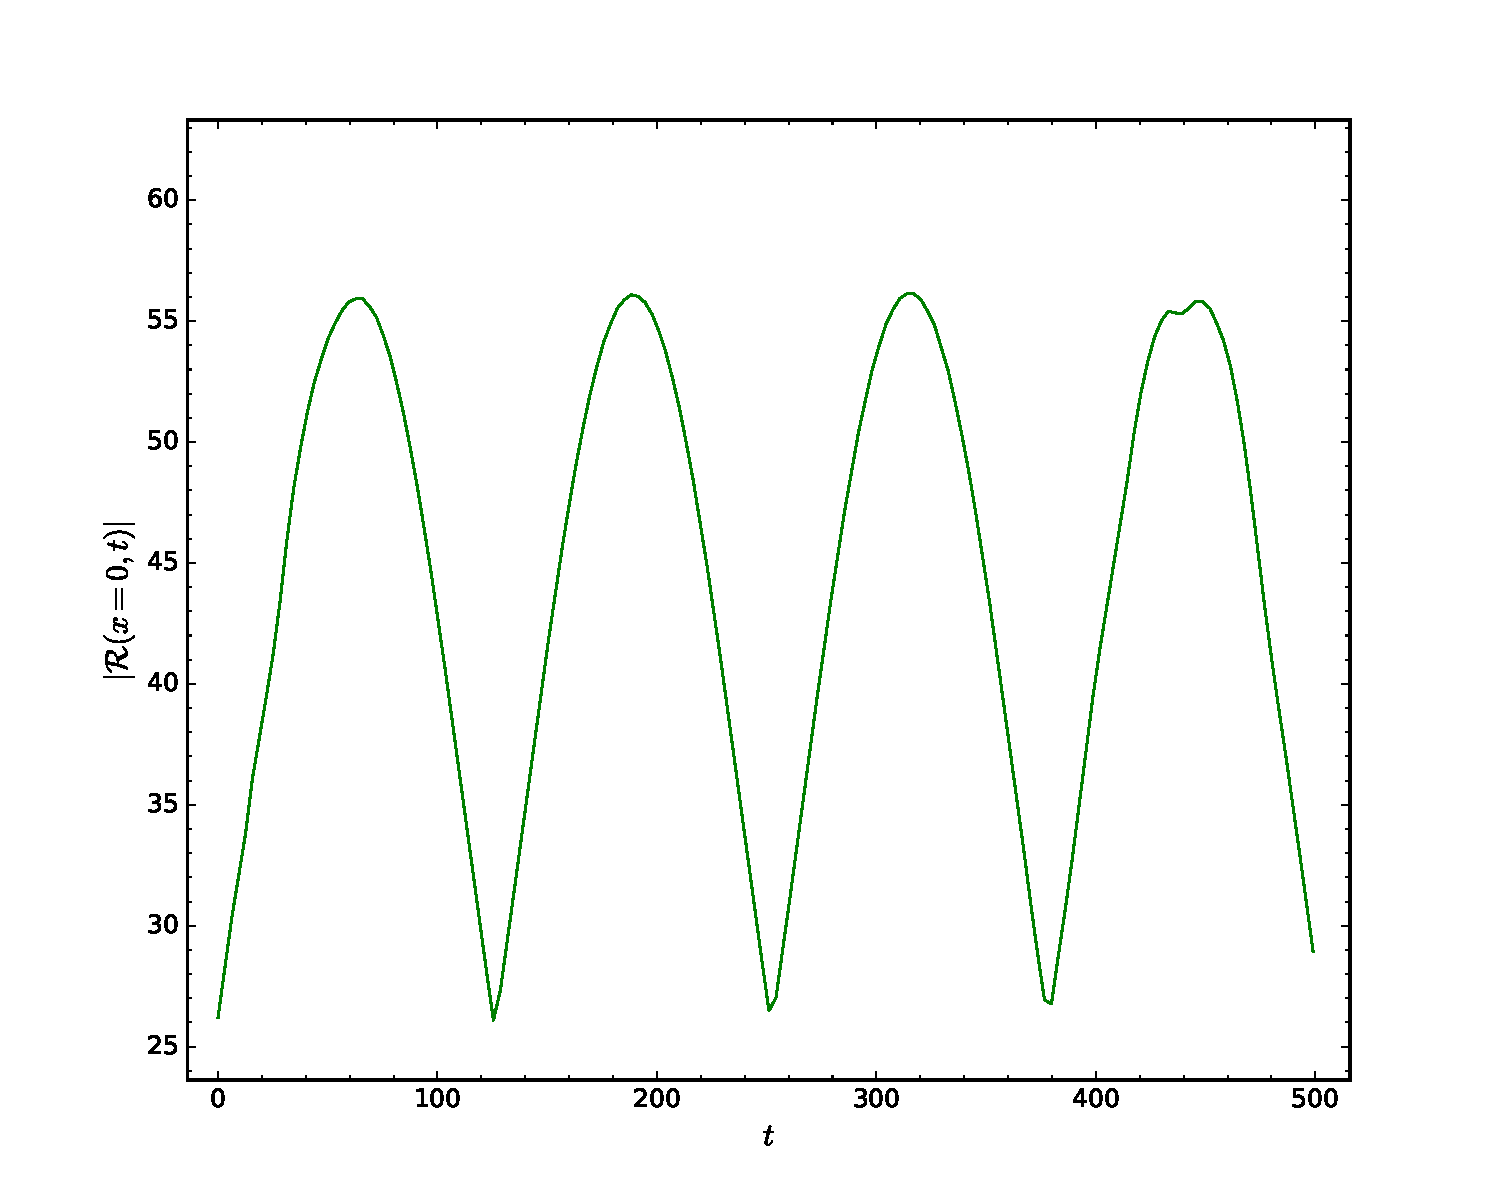
\includegraphics[width=\textwidth]{/Users/bradc/Research/Thesis/PhD/Chapter2/figs/HighTa4_072e-01padj200T5_3921e+00_ricci}
%		\caption{The upper envelope of the Ricci scalar at the origin per light-crossing time for the padded threshold temperature solution.}
%	\end{subfigure}
%	\caption[Padded threshold temperature solutions cannot be projected back to the QP solution surface]{Despite the spectrum of the padded threshold temperature solution (figure~\ref{fig:HighTa4_072e-01padj200T5_3921e+00_evo}) resembling that of lower-temperature QP solutions, these solutions move away from the QP surface and can no longer be projected back.}
%	\label{fig: HighTa4_072e-01padj200T5_3921e+00_projections}
%\end{figure}



%\begin{figure}[ht]
%	\centering
%	\begin{subfigure}[t]{0.45\textwidth}
%		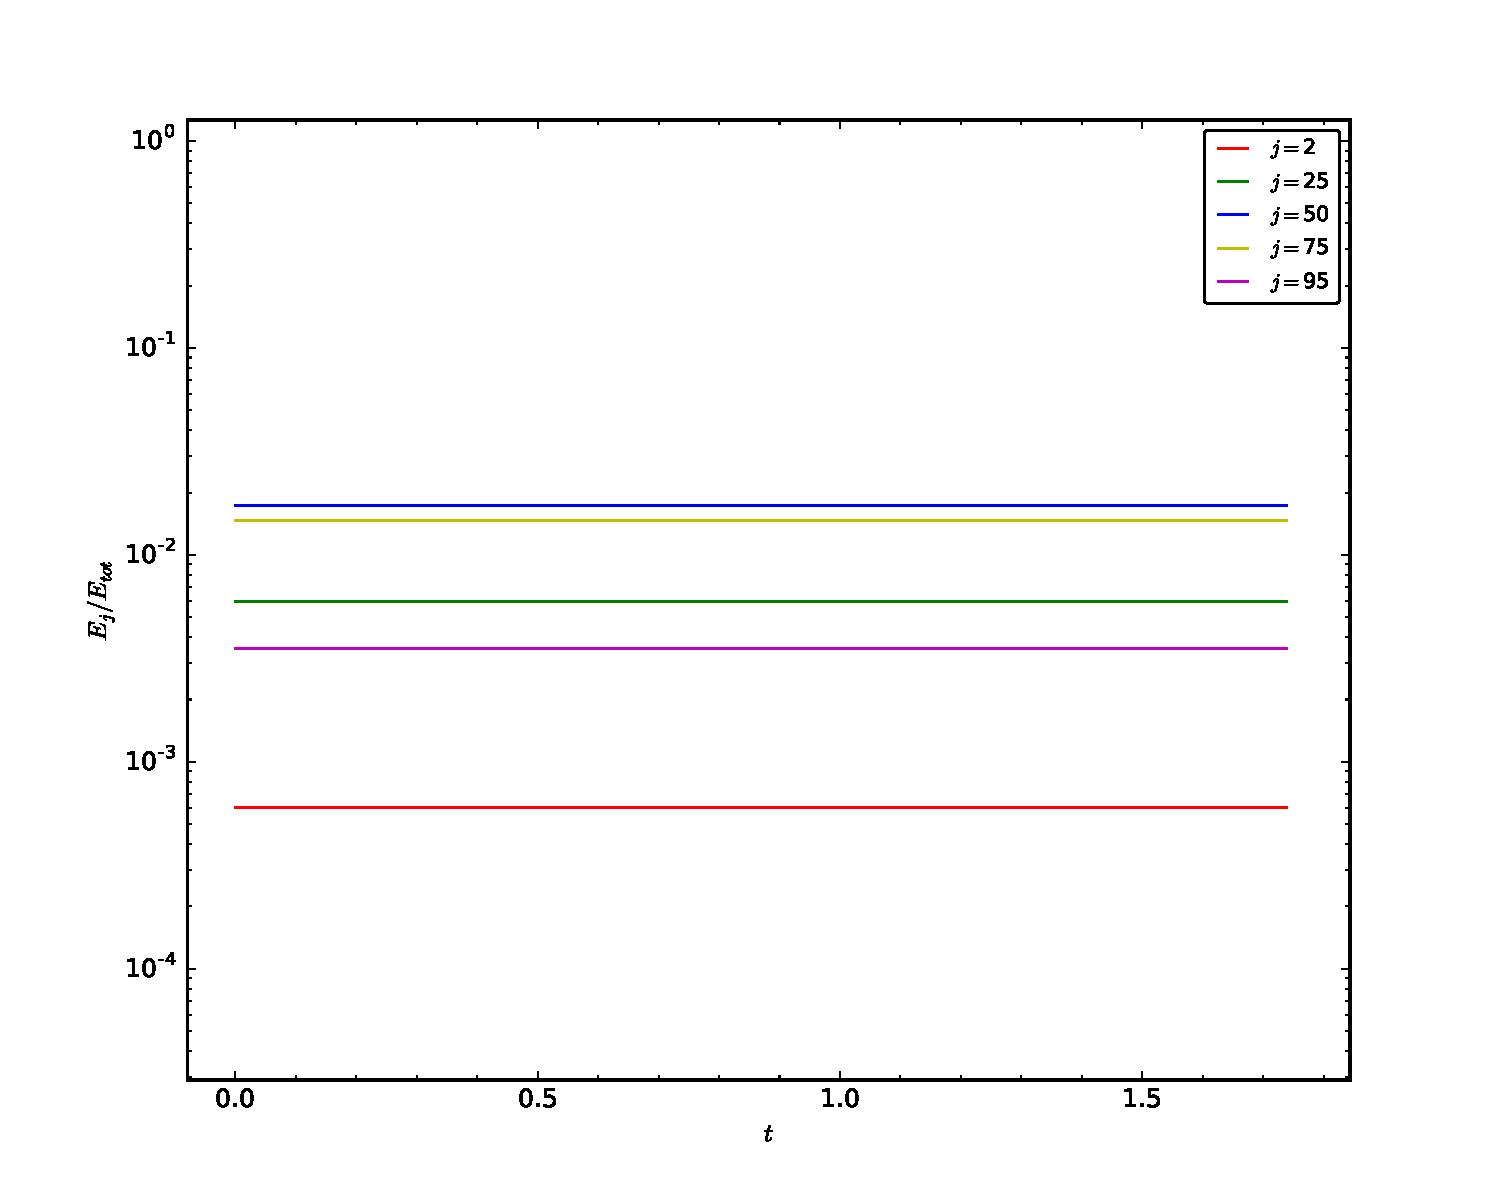
\includegraphics[width=\textwidth]{/Users/bradc/Research/Thesis/PhD/Chapter2/figs/HighTa2_1819e-01j100T6_6711e+01_fullevo}
%	\end{subfigure}
%	\;
%	\begin{subfigure}[t]{0.45\textwidth}
%		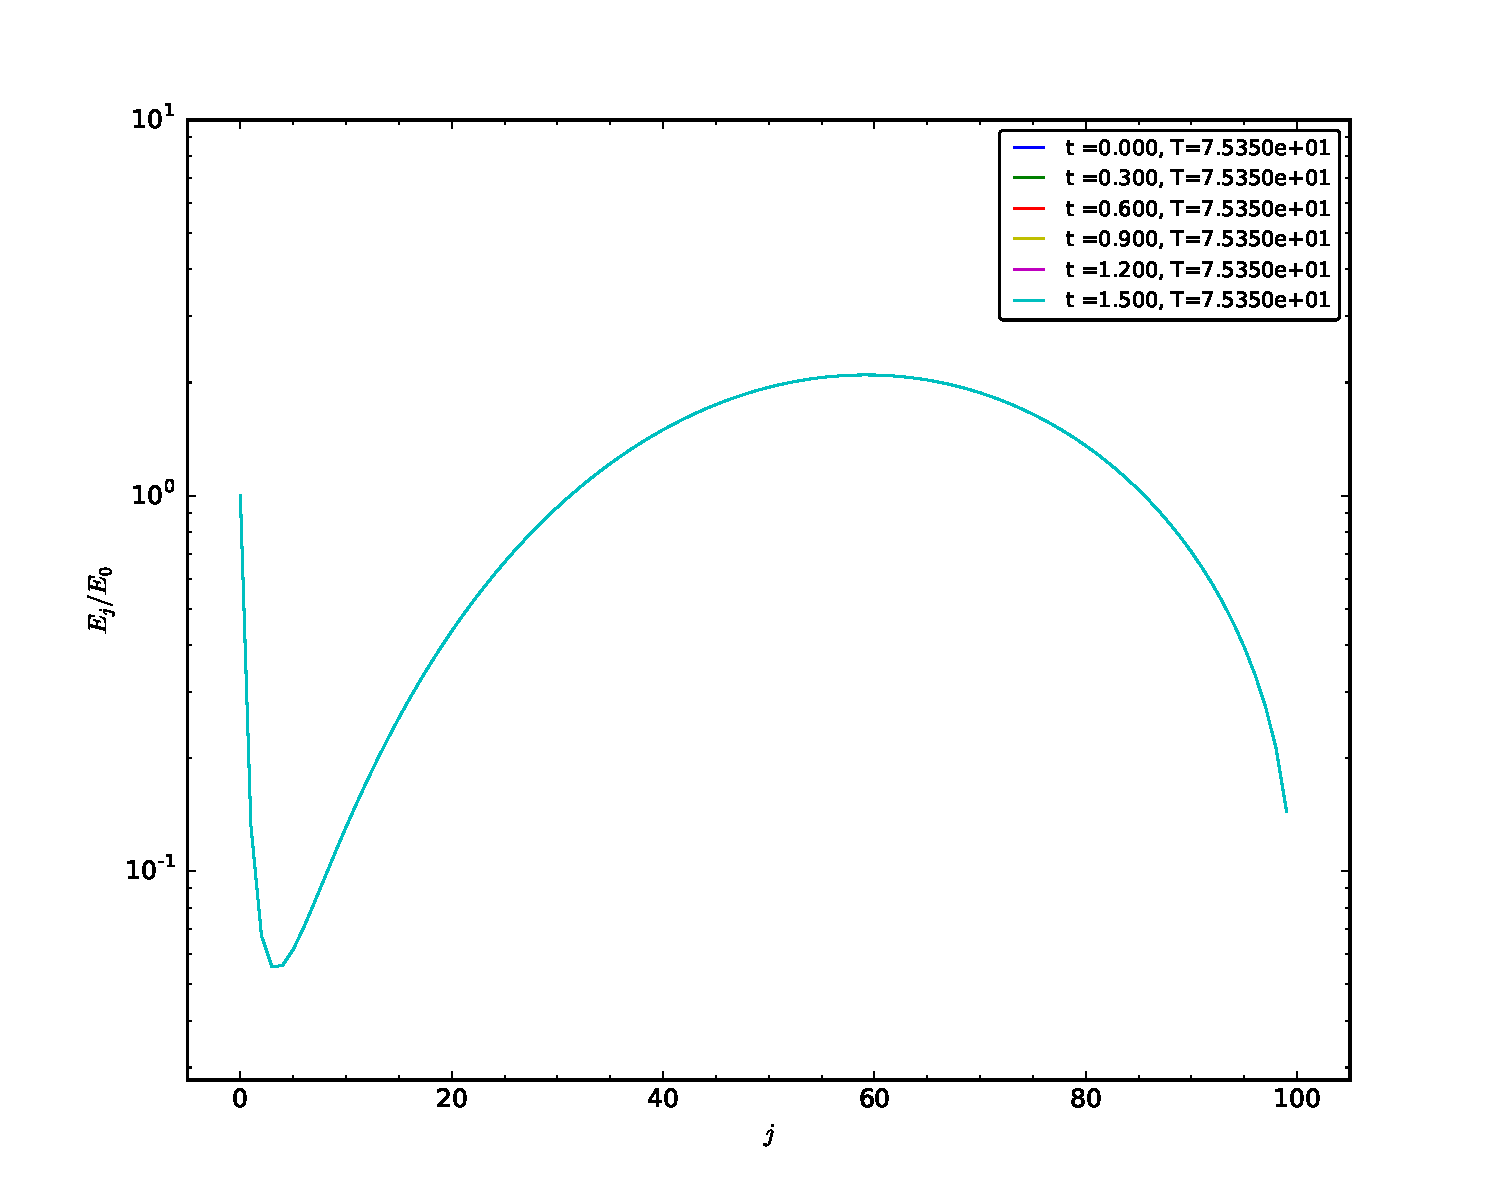
\includegraphics[width=\textwidth]{/Users/bradc/Research/Thesis/PhD/Chapter2/figs/HighTa2_1819e-01j100T6_6711e+01_specevo}
%	\end{subfigure}
%	\caption[Evolution of the energy spectrum for a high-temperature solution created by hand]{The evolution of a high-temperature solution created by hand from lower $\jm$ solutions.}
%	\label{fig: HighTa2_1819e-01j100T6_6711e+01}
%\end{figure}


%\begin{figure}[ht]
%	\centering
%	\begin{subfigure}[t]{0.45\textwidth}
%		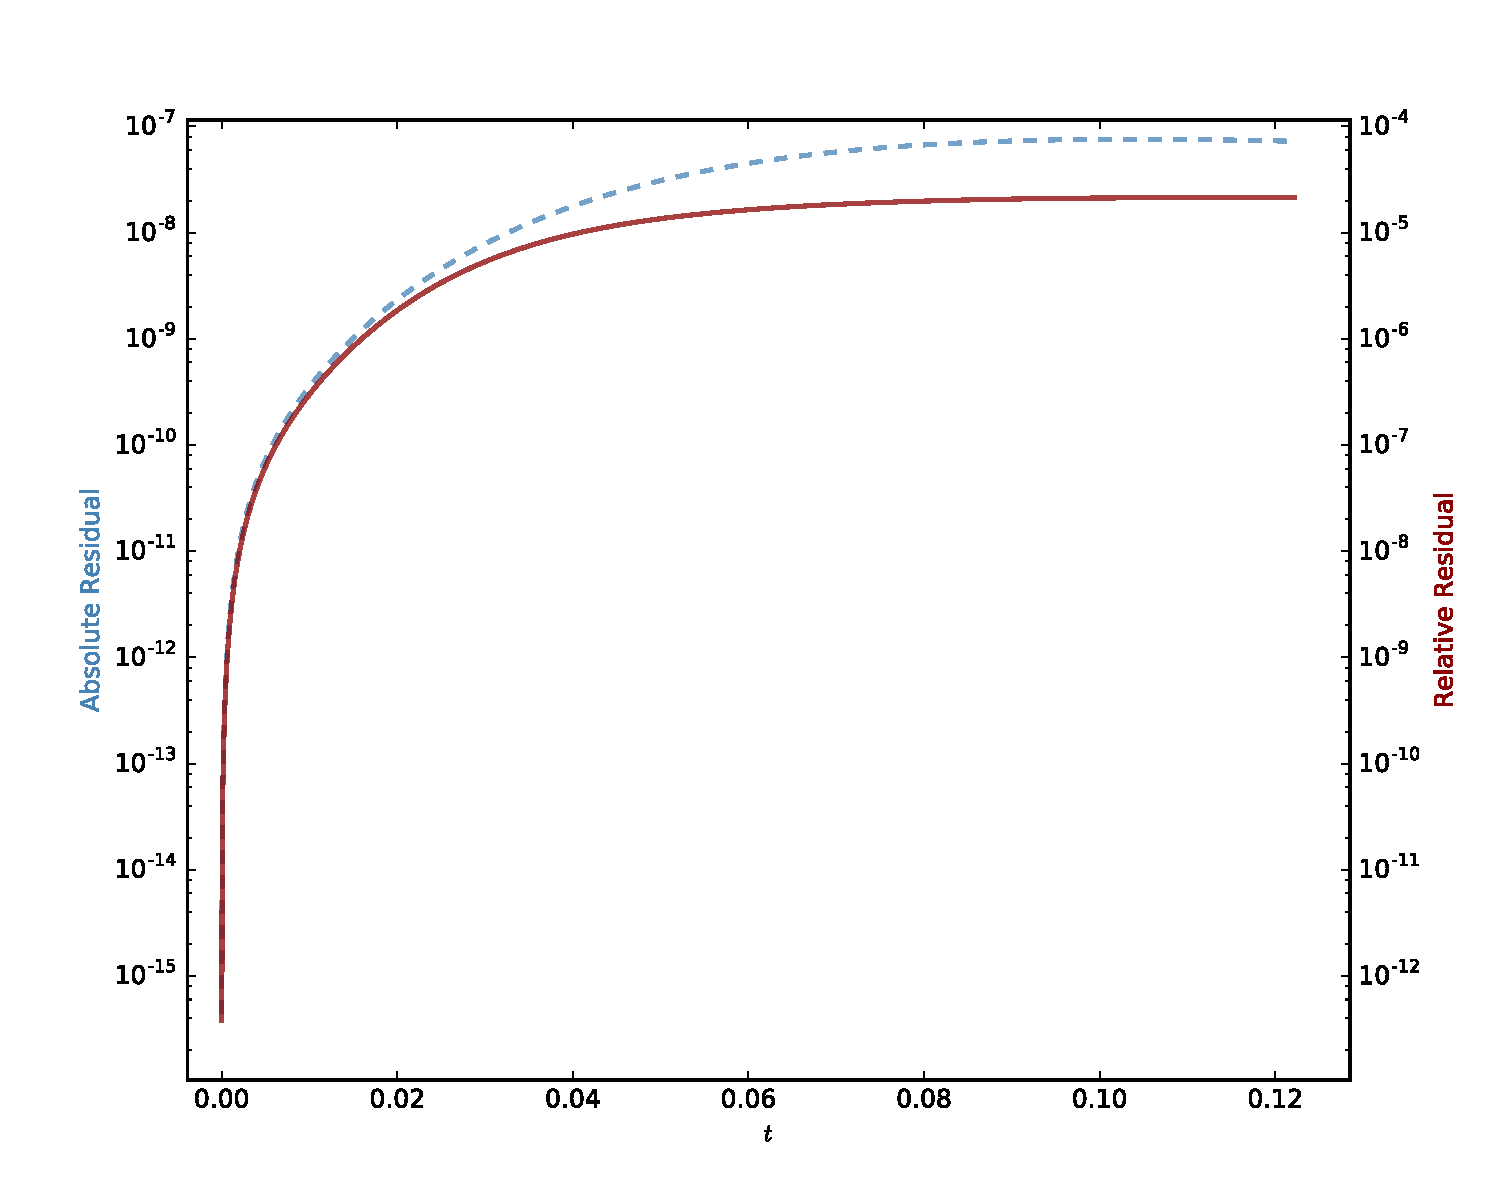
\includegraphics[width=\textwidth]{/Users/bradc/Research/Thesis/PhD/Chapter2/figs/Qpa4_40e-01j100EEresids}
%		\caption{An $\alpha_1 = 0.44$, $\jm = 100$ QP solution with $\epsilon = 0.001$.}
%		\label{fig:QPEEresid}
%	\end{subfigure}
%	\;
%	\begin{subfigure}[t]{0.45\textwidth}
%		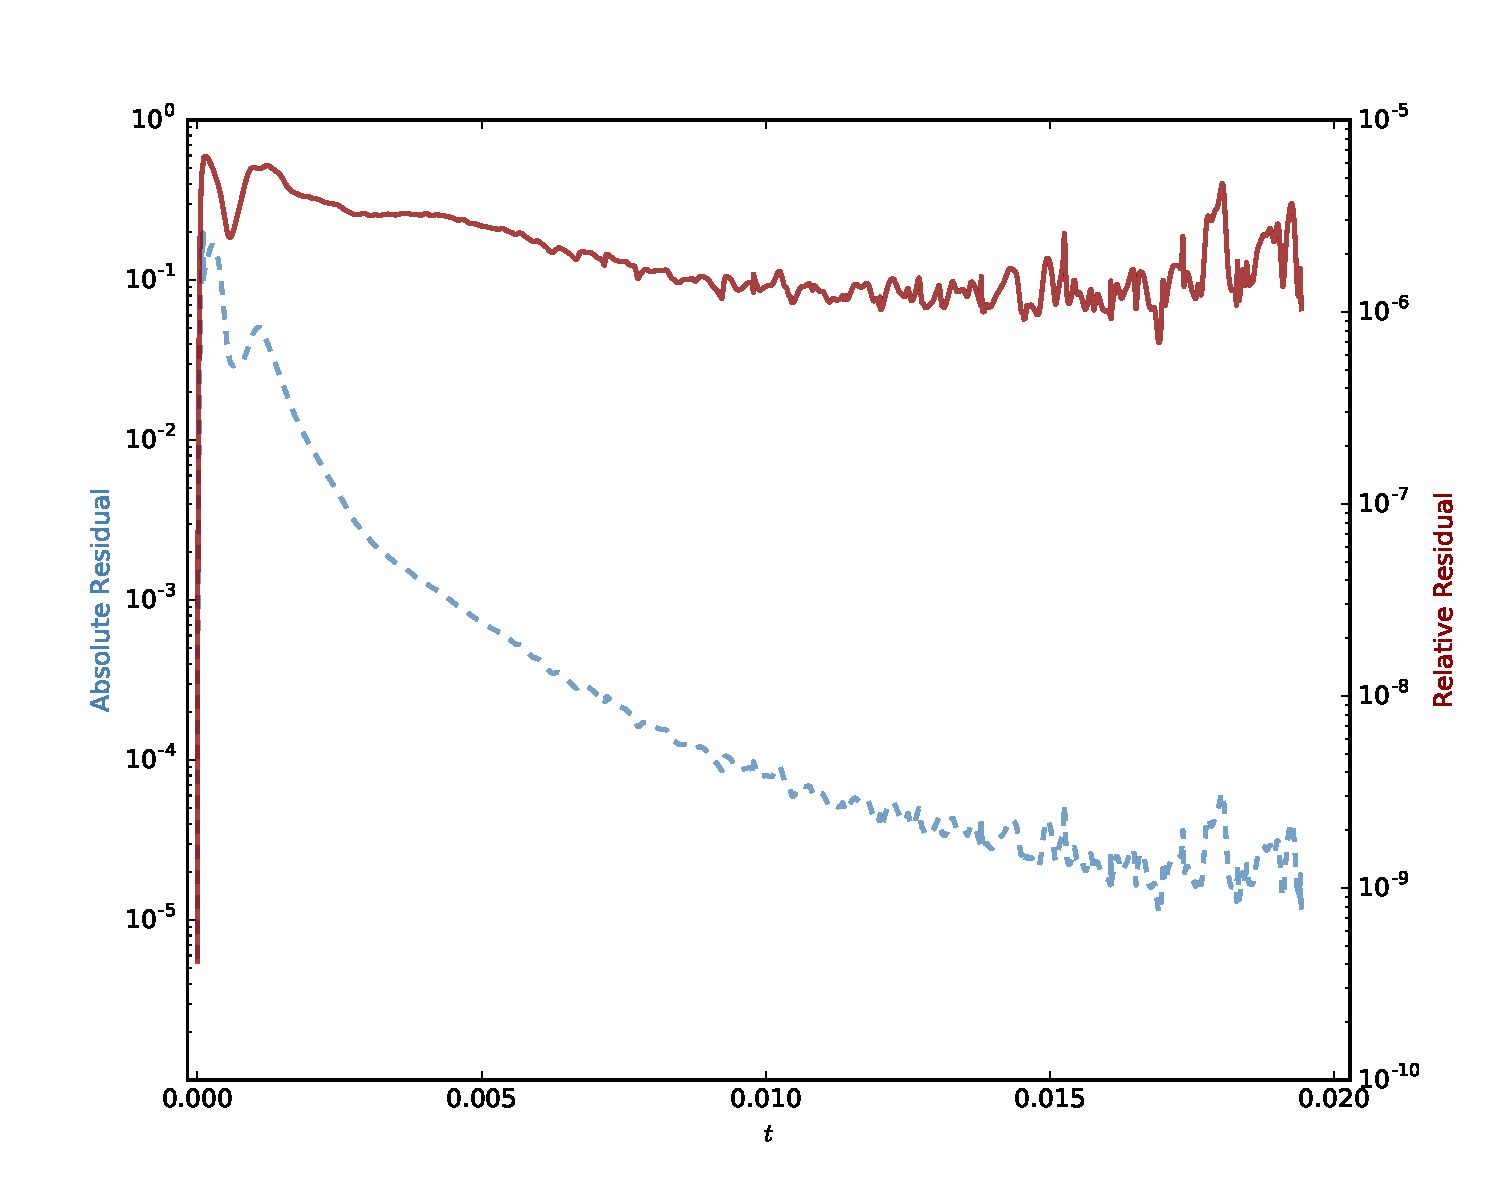
\includegraphics[width=\textwidth]{/Users/bradc/Research/Thesis/PhD/Chapter2/figs/HighTa2_1819e-01padj125T6_6711e+01_EEresids}
%		\caption{A $\jm = 100$, high-temperature solution is padded with zeros to $\jm = 125$ and evolved with $\epsilon = 0.001$.}
%		\label{fig:highTEEresid}
%	\end{subfigure}
%	\caption[Absolute and relative residuals for low- and high-temperature QP solutions]{Residuals from evaluating the constraints for QP and high temperature solutions.}
%	\label{fig:EEresids}
%\end{figure}

%Attempt padding out to $\jm = 125$ and run the evolution: see figure~\ref{fig:HighTa2_1819e-01padj125T6_6711e+01_evo}
%\begin{figure}[ht]
%	\centering
%	\begin{subfigure}[t]{0.45\textwidth}
%		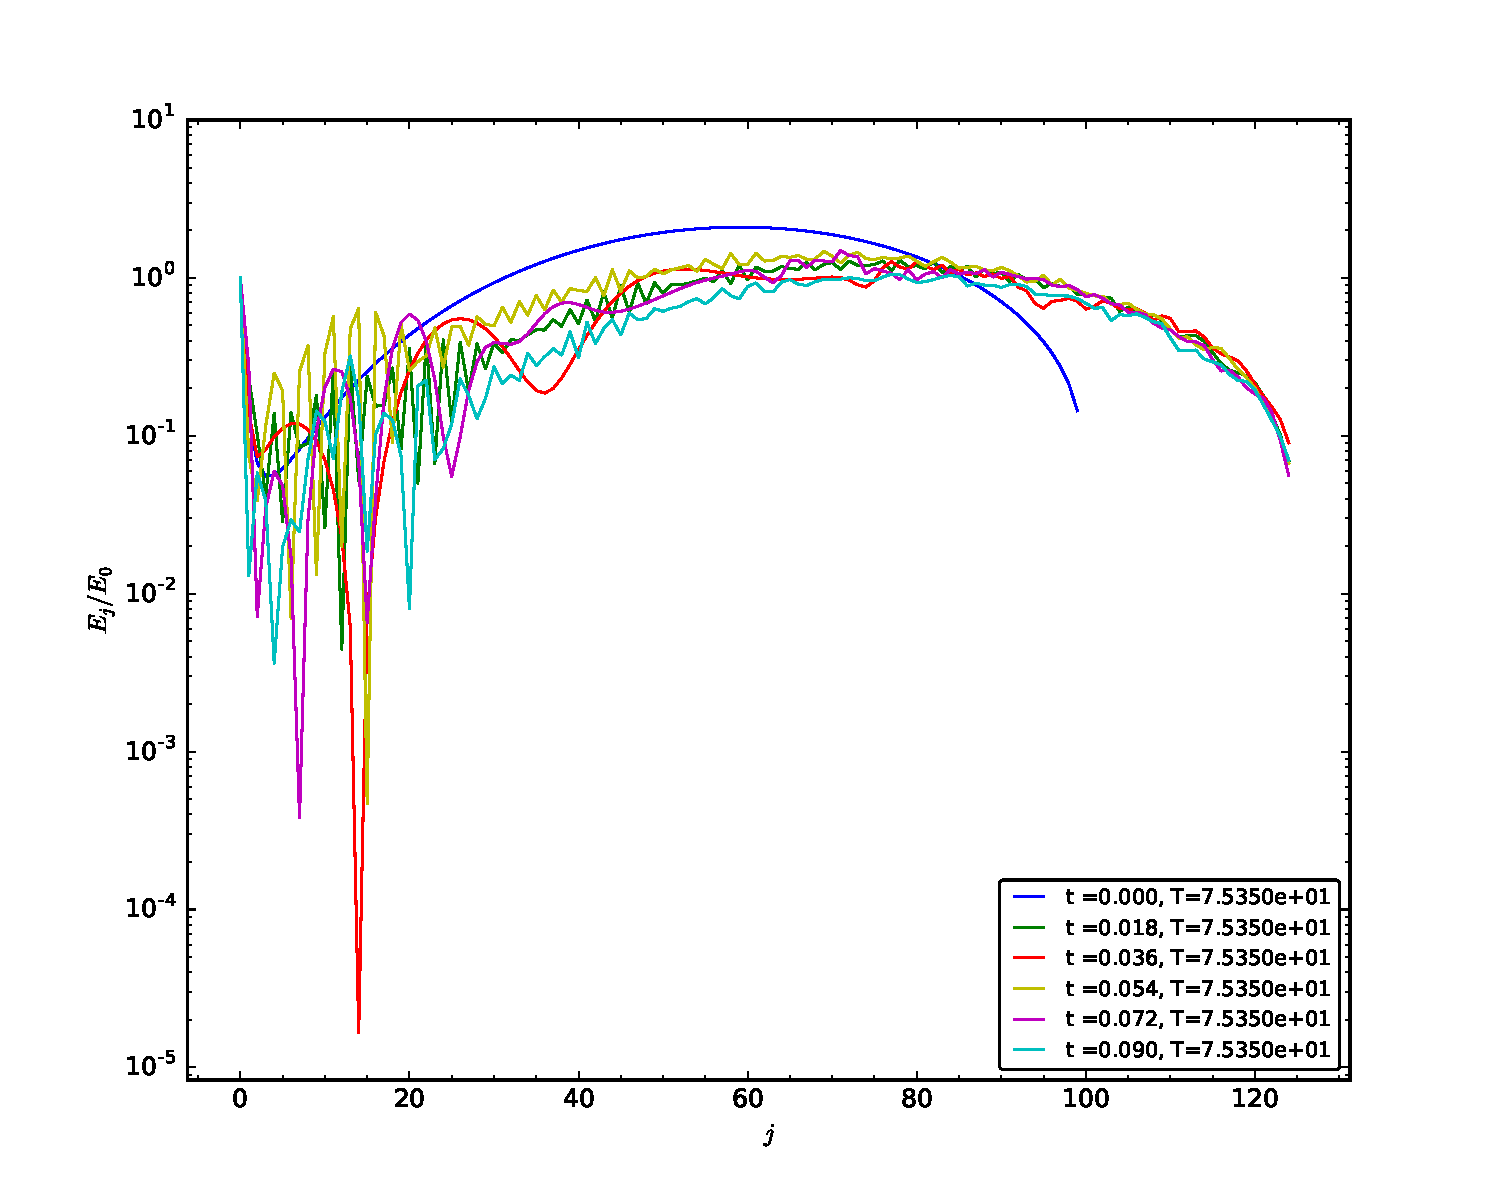
\includegraphics[width=\textwidth]{/Users/bradc/Research/Thesis/PhD/Chapter2/figs/HighTa2_192e-01padj125T6_6711e+01_spectrumevo}
%	\end{subfigure}
%	\;
%	\begin{subfigure}[t]{0.45\textwidth}
%		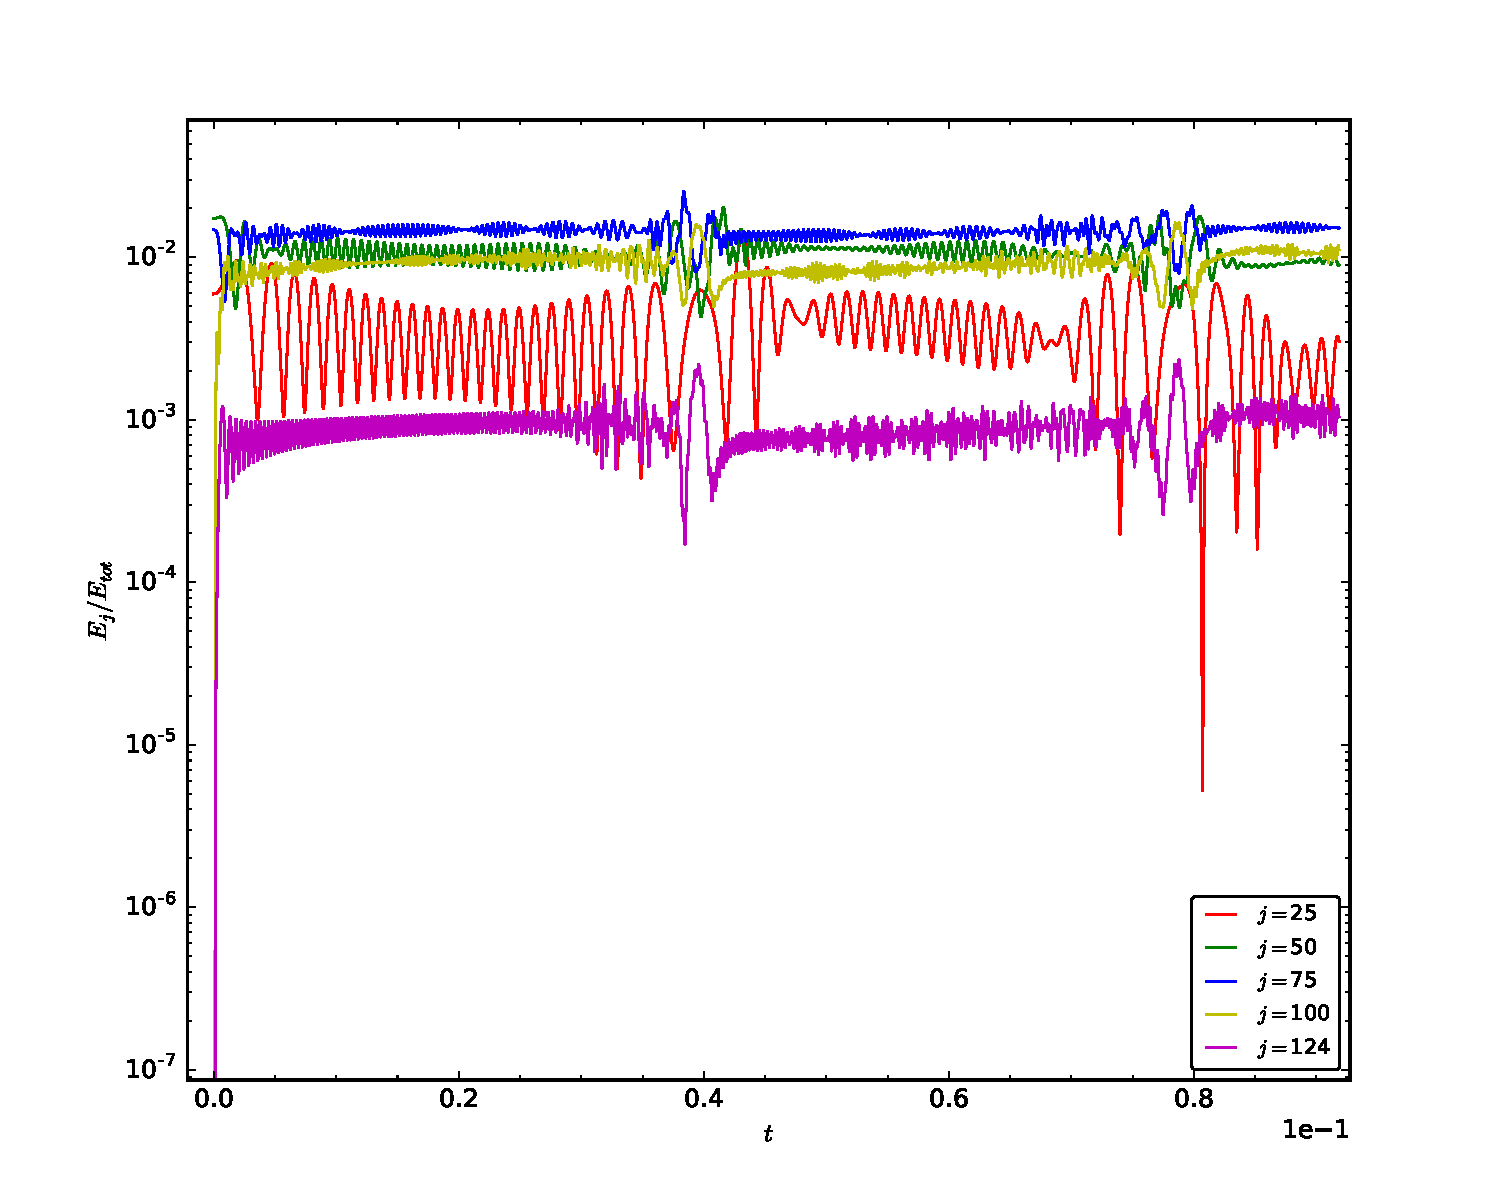
\includegraphics[width=\textwidth]{/Users/bradc/Research/Thesis/PhD/Chapter2/figs/HighTa2_192e-01padj125T6_6711e+01_fullevo}
%	\end{subfigure}
%	\;
%	\begin{subfigure}[t]{0.45\textwidth}
%		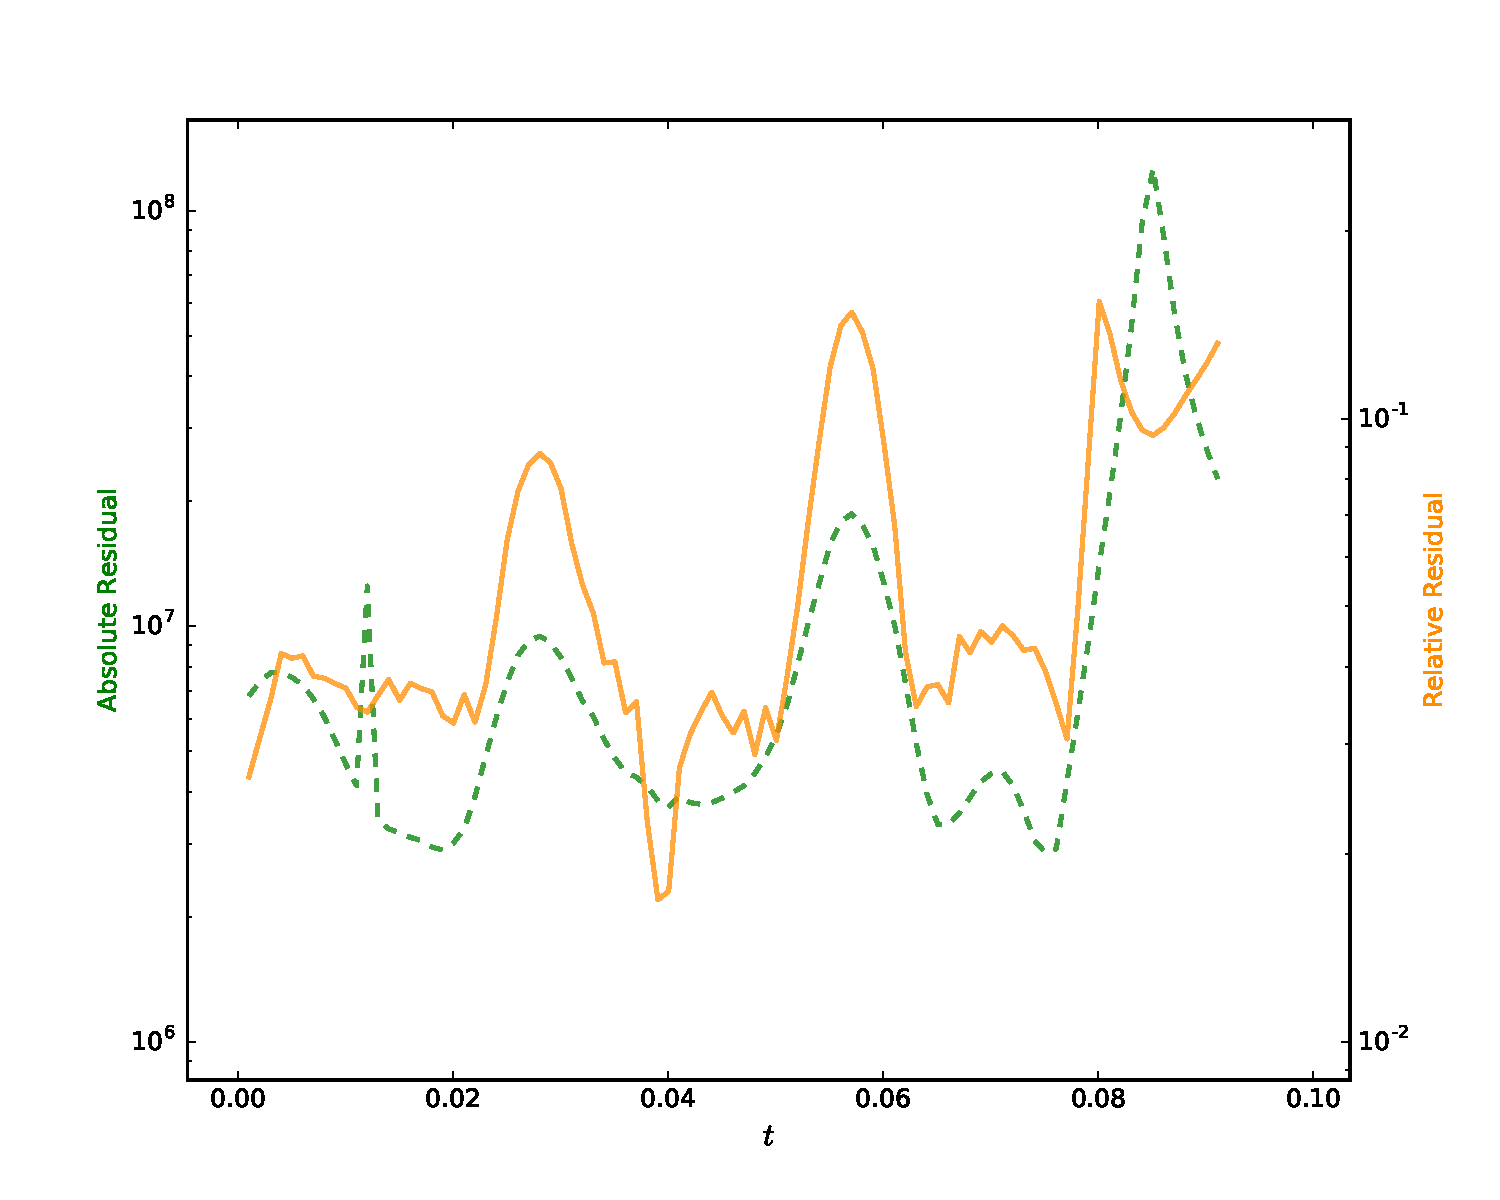
\includegraphics[width=\textwidth]{/Users/bradc/Research/Thesis/PhD/Chapter2/figs/HighTa2_1819e-01padj125T6_6711e+01_Qpresids}
%	\end{subfigure}
%	\;
%	\begin{subfigure}[t]{0.45\textwidth}
%		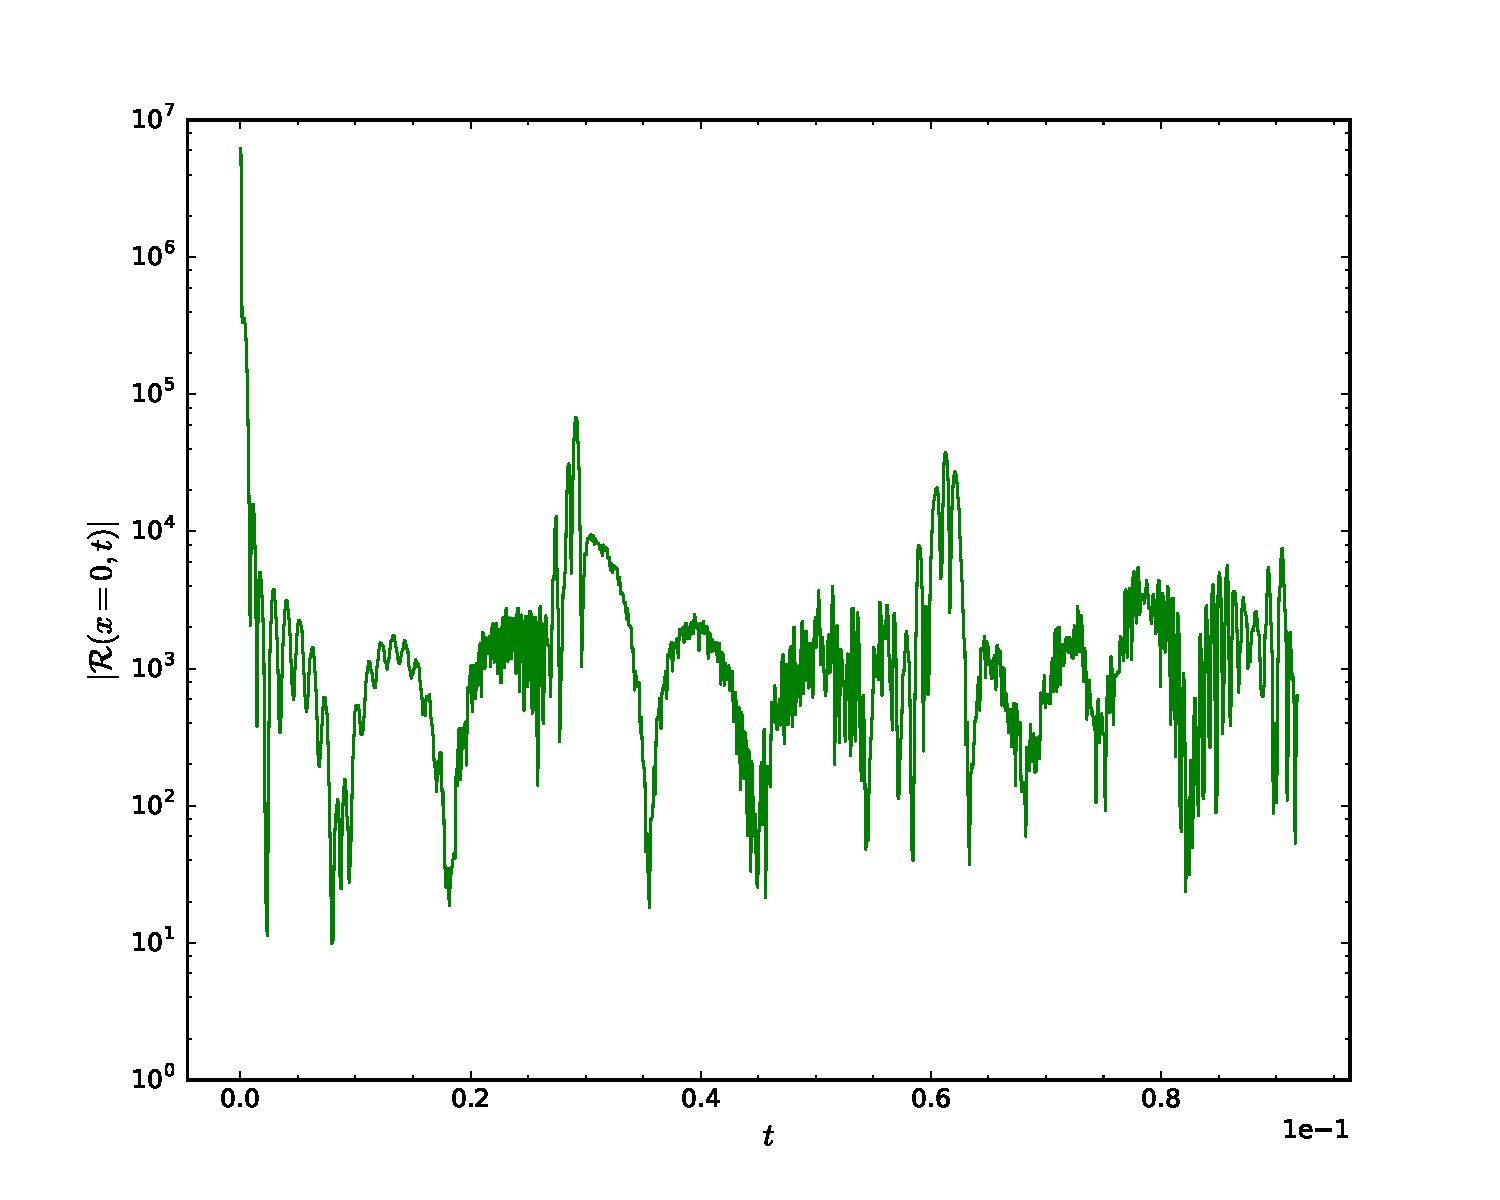
\includegraphics[width=\textwidth]{/Users/bradc/Research/Thesis/PhD/Chapter2/figs/HighTa2_1819e-01padj125T6_6711e+01_ricci}
%	\end{subfigure}
%	\caption[Evolution of the spectrum, absolute and relative residual, and Ricci scalar for a high-temperature solution that has been padded with $25$ extra modes]{Padding the same initial solution from figure~\ref{fig: making highT}, but with only $25$ extra modes.}
%	\label{fig:HighTa2_1819e-01padj125T6_6711e+01_evo}
%\end{figure}

%Finally, consider padding such a solution out to $\jm = 200$. See figure~\ref{fig:HighTa2_1819e-01padj200T6_6711e+01_evo} for results.
%\begin{figure}[ht]
%	\centering
%	\begin{subfigure}[t]{0.45\textwidth}
%		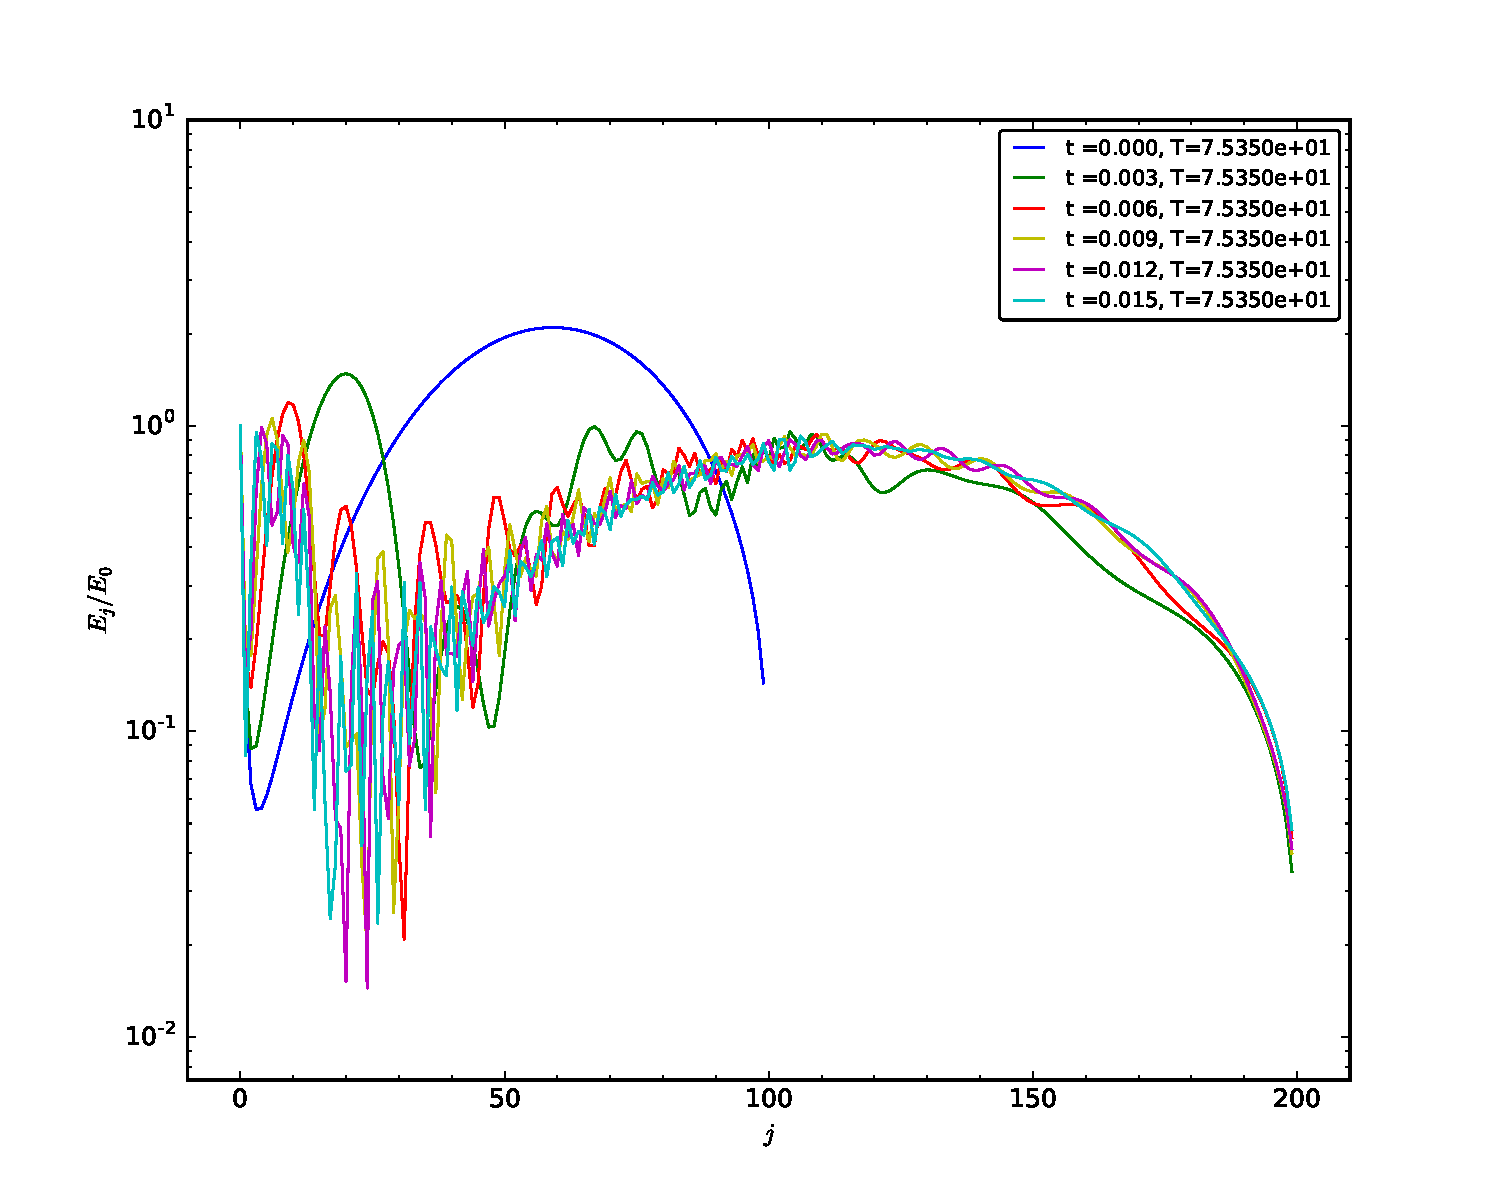
\includegraphics[width=\textwidth]{/Users/bradc/Research/Thesis/PhD/Chapter2/figs/HighTa2_1819e-01padj200T6_6711e+01_specevo}
%	\end{subfigure}
%	\;
%	\begin{subfigure}[t]{0.45\textwidth}
%		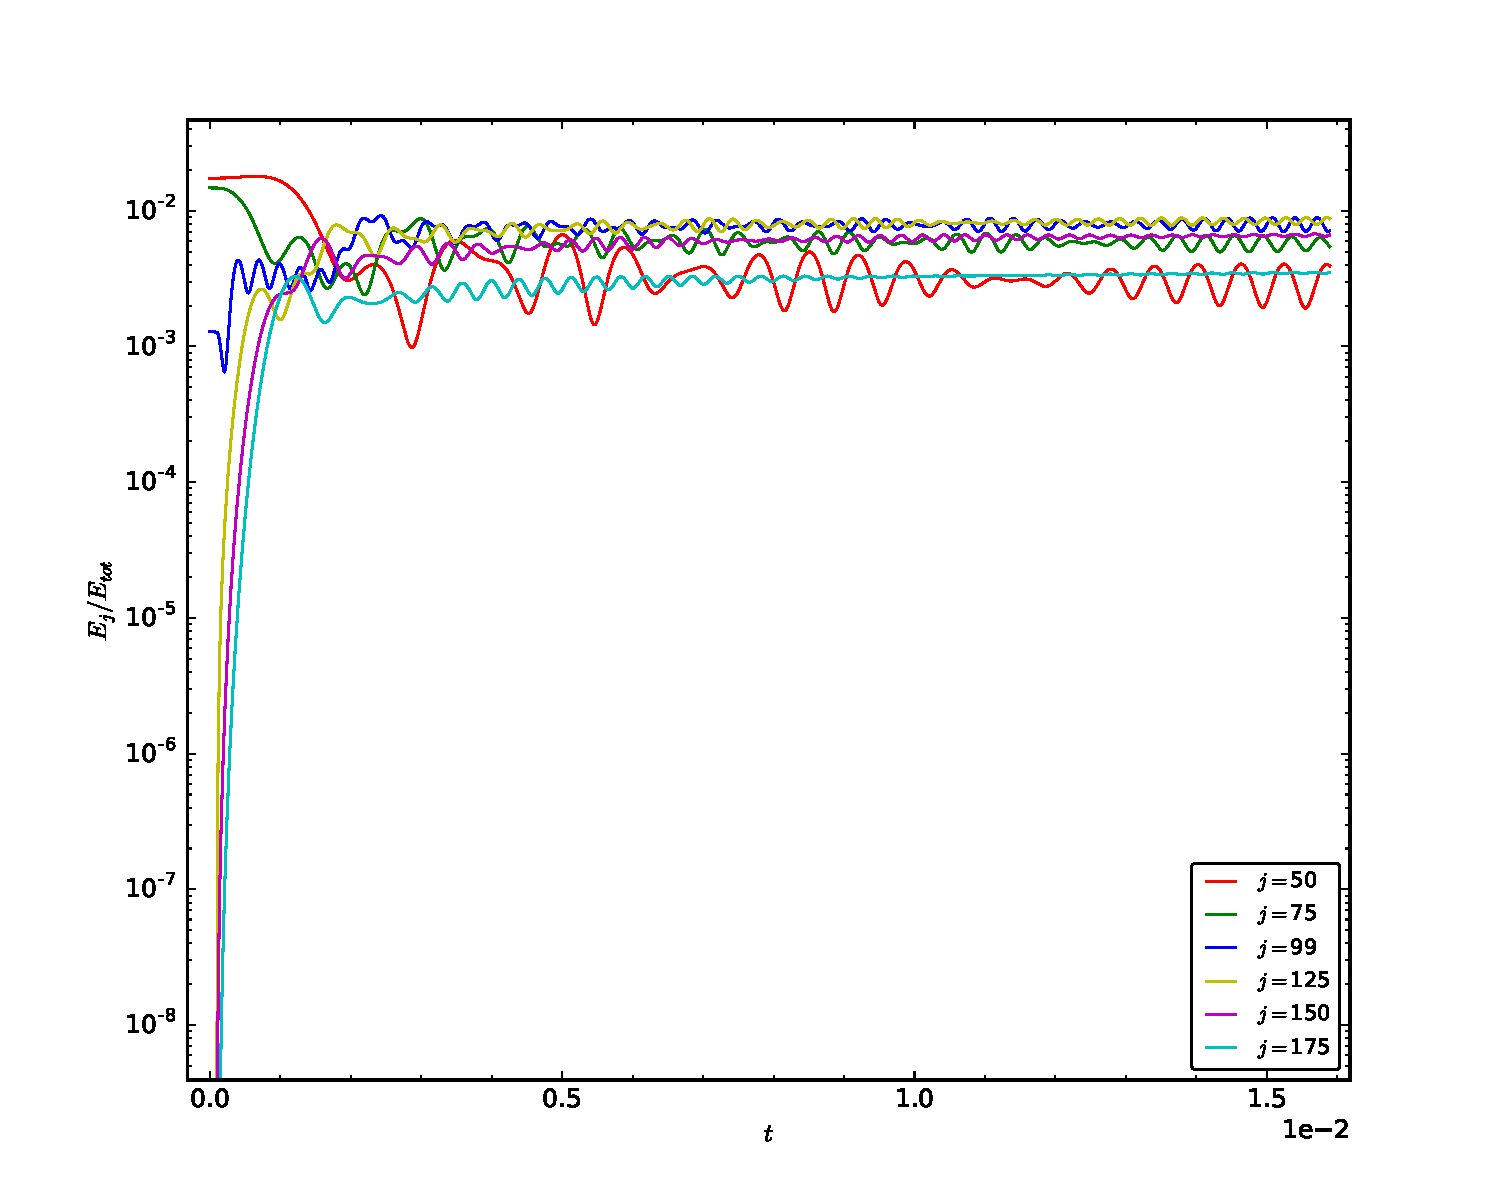
\includegraphics[width=\textwidth]{/Users/bradc/Research/Thesis/PhD/Chapter2/figs/HighTa2_1819e-01padj200T6_6711e+01_modesevo}
%	\end{subfigure}
%	\caption[Evolution of the spectrum of a high-temperature solution padded with $100$ modes]{Padding a $\jm = 100$, high temperature solution to $\jm = 200$ and evolving in time. $\epsilon = 0.1$}
%	\label{fig:HighTa2_1819e-01padj200T6_6711e+01_evo}
%\end{figure}

%The evolved profile of the high-temperature solution can no longer be projected back to the QP solution surface: figure~\ref{fig: HighTa2_1819e-01padj125T6_6711e+01_evolutionprojection}.
%\begin{figure}[ht]
%	\centering
%	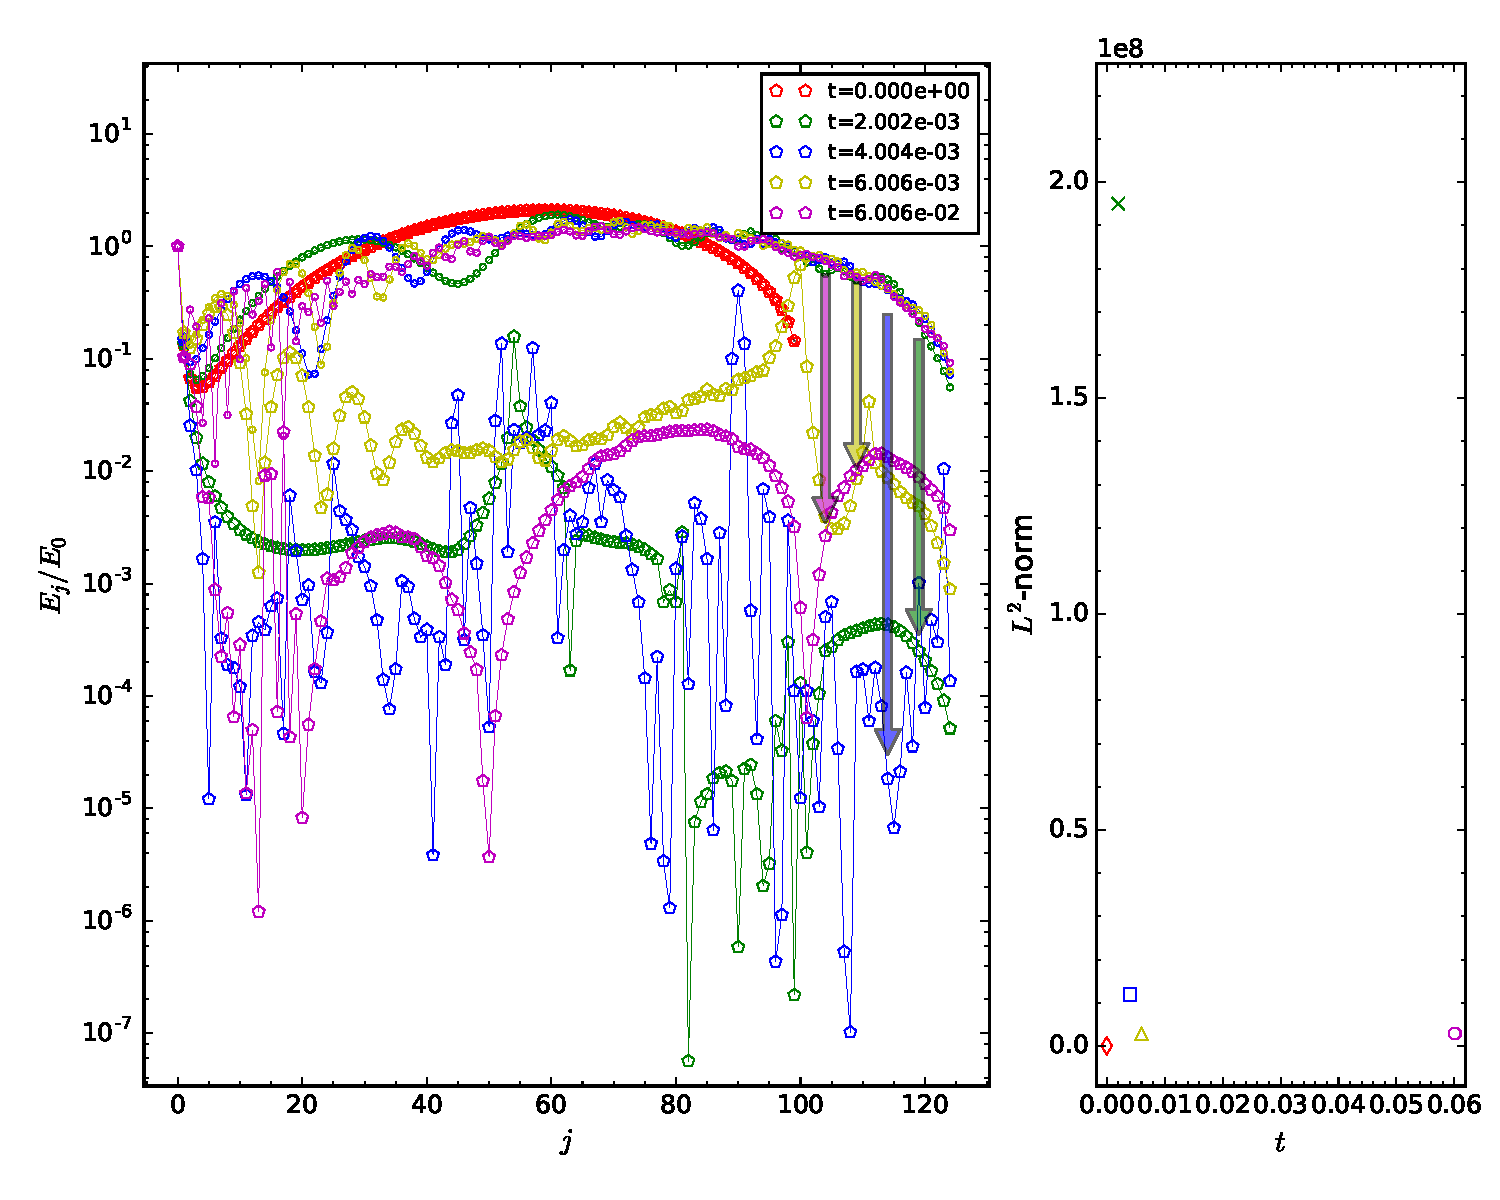
\includegraphics[scale=0.4]{/Users/bradc/Research/Thesis/PhD/Chapter2/figs/HighTa2_1819e-01padj125T6_6711e+01_evolutionprojection}
%	\caption[Evolution of the spectrum of a high-temperature solution padded with $25$ modes]{A high-temperature solution is padded with $25$ extra modes, then evolved in time. Above are the results of projecting back to the QP surface at $t \simeq 0.002, 0.004, 0.006, 0.06$ (red diamond, green cross, blue square, yellow triangle, magenta cirlce).}
%	\label{fig: HighTa2_1819e-01padj125T6_6711e+01_evolutionprojection}
%\end{figure}

%\begin{figure}[ht]
%	\centering
%	\begin{subfigure}[t]{0.45\textwidth}
%		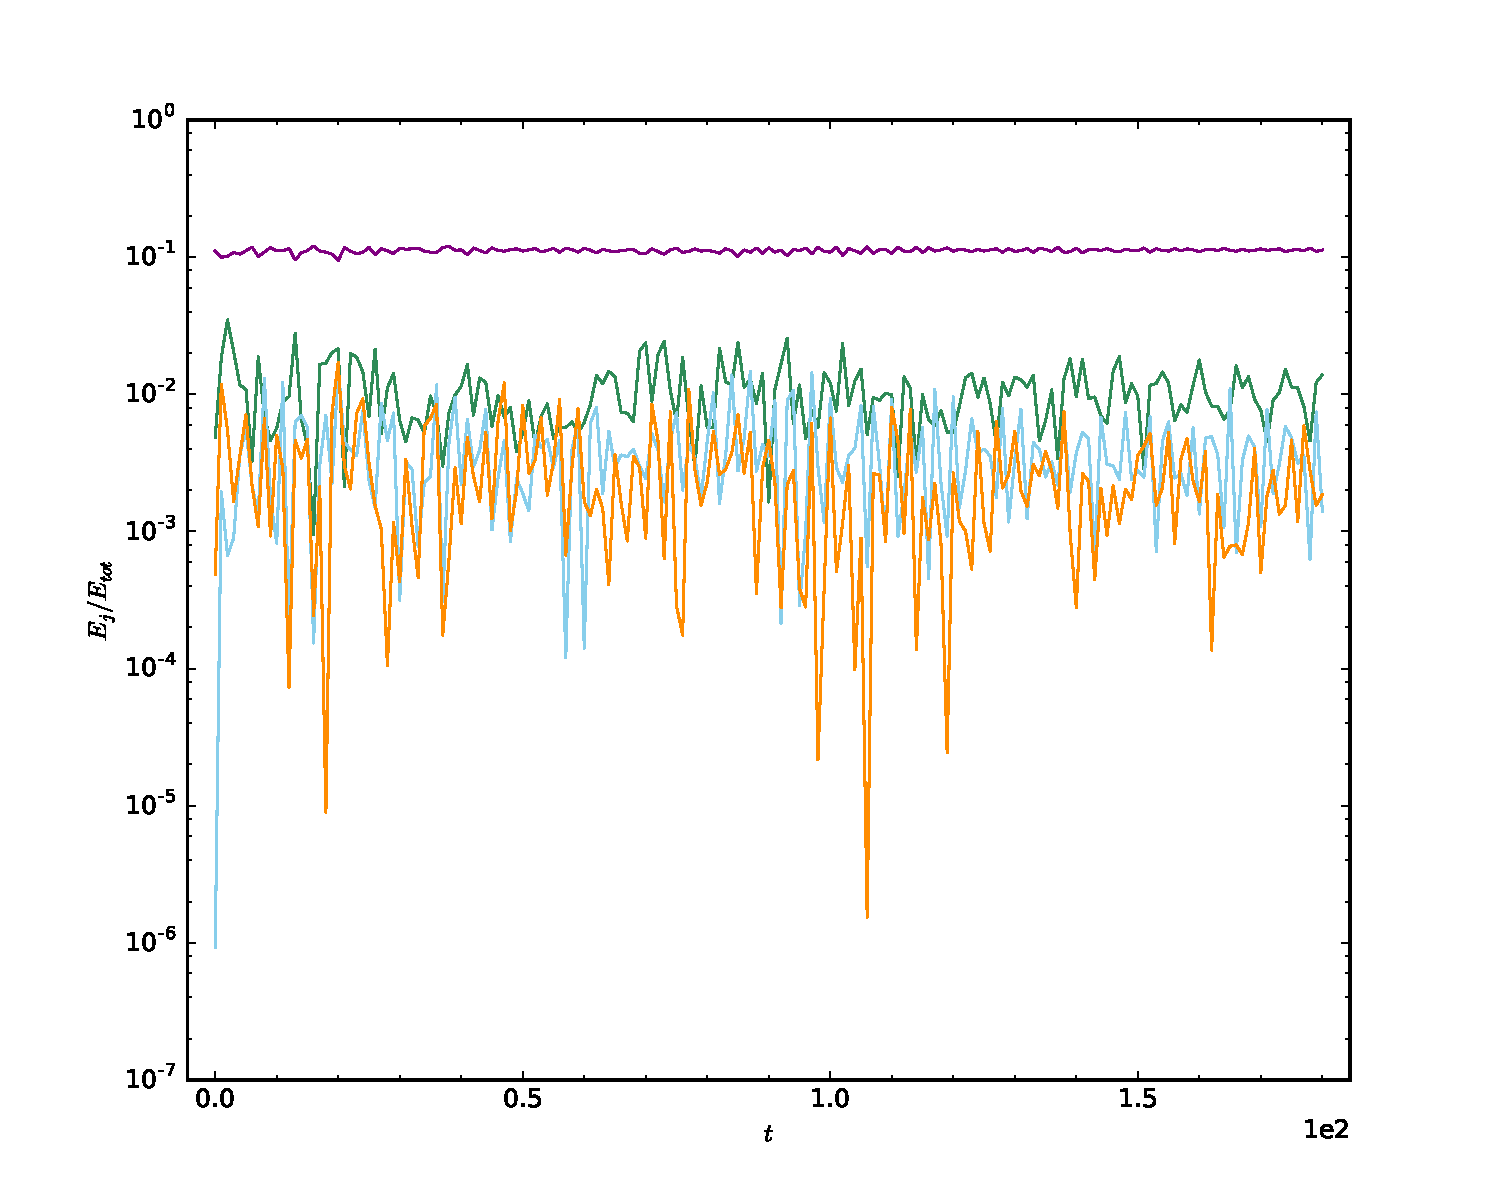
\includegraphics[width=\textwidth]{/Users/bradc/Research/Thesis/PhD/Chapter2/figs/HighTa1_779e-01j100T2_0000e+01_lowjevo}
%		\caption{Evolution of the first four modes: ${j = 0, 1, 2, 3}$ (purple, green, blue, orange).}
%	\end{subfigure}
%	\;
%	\begin{subfigure}[t]{0.45\textwidth}
%		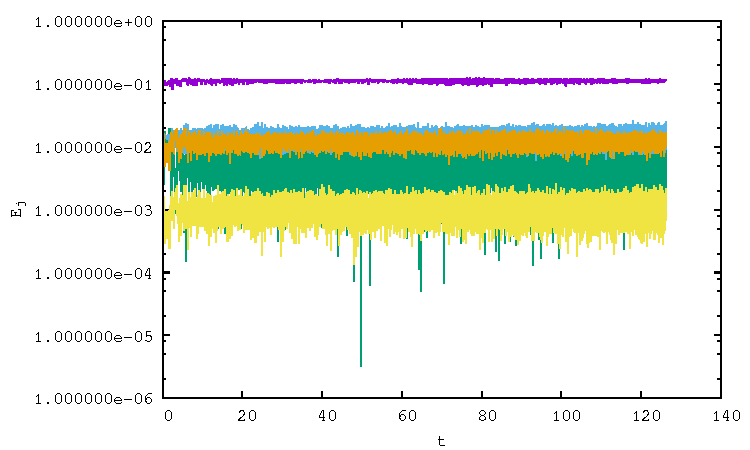
\includegraphics[width=\textwidth]{/Users/bradc/Research/Thesis/PhD/Chapter2/figs/HighTa1_779e-01j100T2_0000e+01_fullevo}
%		\caption{Comparative evolution of modes ${j=0, 25, 50, 75, 99}$ (purple, green, blue, orange, yellow).}
%	\end{subfigure}
%	\;
%	\begin{subfigure}[t]{0.45\textwidth}
%		\includegraphics[width=\textwidth]{/Users/bradc/Research/Thesis/PhD/Chapter2/figs/HighTa1_779e-01j100T2_0000e+01_specevo}
%		\caption{Energy spectrum at selected times throughout the evolution.}
%	\end{subfigure}
%	\;
%	\begin{subfigure}[t]{0.45\textwidth}
%		\includegraphics[width=\textwidth]{/Users/bradc/Research/Thesis/PhD/Chapter2/figs/HighTa1_779e-01j100T2_0000e+01_Ricci}
%		\caption{The upper envelope of the Ricci scalar at the origin, per light-crossing time.}
%	\end{subfigure}
%	\caption[Evolution of a high-temperature state that does not satisfy the QP equation]{The evolution of an intermediate, high-temperature solution that \emph{does not} correspond to a solution of the QP equations.}
%	\label{fig:HighTa1_779e-01j100T2_0000e+01evo}
%\end{figure}


%%%%%%%%%%%%%%%%%%%%%%%%%%%%%%%%%%%%%%%%%
%%%%%%%%%%%%%%%%%%%%%%%%%%%%%%%%%%%%%%%%%

\section{Discussion}
\label{sec: ttf discussion}

We have explored the space of quasi-periodic solutions within the perturbative description of a massless scalar field in AdS$_4$. Using the conserved quantities $E$ and $N$, we constructed families of quasi-periodic solutions that were distinguished by the temperature $T = E/N$ for different choices of the truncation value $\jm$. We have demonstrated that low temperature QP solutions, i.e. those that are clearly accessible by solving \eqref{qp eqn} for a given $\alpha_1$ such that $\alpha_1 < \alpha_0 = 1$, can be extended to arbitrarily large $\jm$ values, and therefore constitute solutions to the TTF theory. We have also examined high temperature QP solutions, which are found by perturbing low temperature solutions by $\delta E$ while keeping $N$ fixed. We found that high temperature solutions were robust against increasing $\jm$ only for temperatures $T \lesssim 5.5$. We also applied several alternative methods for generating high temperature QP solutions. However, we were not able to find evidence of any solutions that could be extended to the untruncated TTF system. We constructed low-$\jm$ solutions with $T \gg 5.5$, but found that they were not robust with increasing $\jm$ and therefore were not true solutions. Rather, only solutions with temperatures $T \lesssim 5.5$ could be extended to large $\jm$ values. The nature of this temperature threshold is not totally understood. It may be due to numerical limitations with the Newton-Raphson solving method, or it may be a physical limitation of the quasi-periodic ansatz.

By construction, TTF solutions are stable against gravitational collapse and therefore evolution within the TTF description will not produce a singularity. However, there are several indicators for instability in the fully nonlinear theory: the value of the Ricci scalar at the origin, the growth higher-order contributions to the lapse function $\delta$, and rapid growth/oscillations in the energy of high frequency modes. With these indicators in mind, we have shown that low temperature QP solutions constructed from directly solving \eqref{qp eqn} did produce oscillations in $\mc R$, however they did not exhibit other behaviour -- such as the rapid transfer of energy from low- to high-frequency components -- that would suggest instability in the fully nonlinear theory. At late times in their TTF evolution, these solutions project back to the QP surface without altering their energy spectra. 

In an effort to find QP solutions through extensions of known solutions, we constructed seed data from low temperature QP solutions that had been padded with extra, zero-energy modes. However, attempting to project back to the solution surface resulted either in solutions that were not robust as $\jm$ was increased, or failure to find any solution at all. When these data were taken as initial conditions for evolution within the TTF description, no new solutions were found as a result of the evolution. Instead, the inclusion of extra modes caused an isothermal drift away from the known QP seed solution and the Newton-Raphson solver was not able to project the data back to the QP surface. In such cases, the scalar curvature became oscillatory with values ranging up to $20$ times the initial curvature. Padding $T \simeq 5.4$ QP solutions with zero-energy modes once again produced an isothermal drift during evolution and did not converge towards the known QP solution for that temperature and number of modes. These solutions, however, exhibit slow oscillations of scalar curvature over a narrow range of values, hinting at stability over perturbative timescales in the nonlinear theory. 

With respect to the overall stability of AdS$_4$, as well as the interpretation of stable data in the bulk as non-thermalizing states in the boundary theory, we did not find evidence of families of quasi-periodic solutions with high temperatures that are robust against increasing $\jm$. It is important to note that we have focused entirely on solutions where the dominant energy contribution is in the $j = 0$ mode. Other configurations are possible where the dominant energy contribution is in the $j_r$ mode, with $r \neq 0$. As shown in \cite{1507.08261}, QP solutions for temperatures in certain ranges are degenerate in the value of $r$. It may be that the observed temperature limit for QP data we have seen is an indication that the $r=0$ family of solutions no longer dominates, and instead the correct quasi-periodic solution is one of the $r \neq 0$ families. Now that we have established the tools required to examine this possibility, it will be a focus of future research. Also to be considered in the future is the use of QP solutions as initial data for evolution within the fully nonlinear theory in order to help establish a more precise expression for the perturbative timescale $t_p$. With this, we can create hybrid evolutions for massless scalar field collapses that use TTF methods for evolutions when $t < t_p$ before changing to fully nonlinear methods for $t \geq t_p$. This would decrease the computational power required to study such collapses without compromising the accuracy of the simulation.

%%%%%%%%%%%%%%%%%%%%%%%%%%%%%%%%%%%%%%%%%
%%%%%%%%%%%%%%%%%%%%%%%%%%%%%%%%%%%%%%%%%

\paragraph*{Acknowledgments} The work of ND is supported in part by a Natural Sciences and Engineering
Research Council of Canada PGS-D grant to ND, NSF Grant PHY-1606654 at Cornell University, and by a grant from the Sherman Fairchild Foundation. The work of BC and AF is supported by the Natural Sciences and Engineering Research Council of Canada Discovery Grant program. This research was enabled in part by support provided by WestGrid (\href{www.westgrid.ca}{www.westgrid.ca}) and Compute Canada Calcul Canada (\href{www.computecanada.ca}{www.computecanada.ca}).

%%%%%%%%%%%%%%%%%%%%%%%%%%%%%%%%%%%%%%%%%
%%%%%%%%%%%%%%%%%%%%%%%%%%%%%%%%%%%%%%%%%

\begin{subappendices}

%%%%%%%%%%%%%%%%%%%%%%%%%%%%%%%%%%%%%%%%%
%%%%%%%%%%%%%%%%%%%%%%%%%%%%%%%%%%%%%%%%%

\vspace{-0.15in}

\section{Seeding Methods For Non-Linear Solvers}
\label{app: seeding}
To generate seed values for the $\alpha_j$ with $j \geq 2$, \cite{1507.08261} used the exponential relation
\begin{align}
\label{old seed}
\alpha_j \sim \frac{3 e^{-\mu j}}{2j + 3}
\end{align}
in AdS$_4$, where $\mu = \ln (3 / 5 \alpha_1 )$. However, as $j_{max}$ increased, the seed values diverged significantly from the true solutions (see figure~\ref{fig: solutionfitting} for a comparison between known QP $\alpha_j$ values, the seeds generated by \eqref{old seed}, and the result of the fitting procedure). Although this profile was sufficient for low $j_{max}$ solutions, above $j_{max} \gtrsim 150$, \eqref{old seed} no longer provided an adequate starting guess. To overcome this problem, we applied an exponential fit to the tail values of a known QP solution with lower $j_{max}$. As explained below, this exponential fit was used to extrapolated the data to a higher $j_{max}$. 

\begin{figure}
	\centering
	\includegraphics[width=0.5\textwidth]{/Users/bradc/Research/Thesis/PhD/Chapter2/figs/TailFitPlot}
	\caption{Fitting the tail of the ${\jm = 175}$ spectrum to construct a seed for ${j_{max} = 200}$ at fixed ${\alpha_1 = 0.2}$. Also included is actual QP spectrum for ${j_{max} = 200}$.}
  	\label{fig: tail fitting}
\end{figure}
	
To err on the side of caution, the $\alpha_j$ with ${j \in [ j_{max} - 30, j_{max} - 10]}$ were used from each QP solution to provide more accurate seed values when increasing $\jm$ by 25. See figure~\ref{fig: tail fitting} for a comparison of seed values generated by tail fitting to actual QP solutions. The solutions found using this method of seeding versus those found from the seeding given in \eqref{old seed} had relative differences on the order of $10^{-14}$.

\begin{figure}[ht]
\centering
	\begin{subfigure}[t]{0.45\textwidth}
		\includegraphics[width=\textwidth]{/Users/bradc/Research/Thesis/PhD/Chapter2/figs/SolutionsvsFits_a2_00e-01_pg1}
		\caption{$\alpha_1 = 0.2$ QP solutions for $j_{max} \in [25,100]$.}
		\label{fig: sol vs fit low jmax}
	\end{subfigure}
	\quad
	\begin{subfigure}[t]{0.45\textwidth}
		\includegraphics[width=\textwidth]{/Users/bradc/Research/Thesis/PhD/Chapter2/figs/SolutionsvsFits_a2_00e-01_pg2}
		\caption{$\alpha_1 = 0.2$ QP solutions for $j_{max}~\in~[140,200]$.}
		\label{fig: sol vs fit high jmax}
	\end{subfigure}
	\caption[Comparison of seed values to known QP solutions and exponential fitting]{A comparison of seeds predicted by \eqref{old seed} to known QP solution. Also included for comparison are the results of fitting the QP solutions to a generic exponential fit.}
	\label{fig: solutionfitting}
\end{figure}
			


%\begin{figure}[ht]
%	\centering
%	\begin{subfigure}[t]{0.45\textwidth}
  %		\includegraphics[width=\textwidth]{/Users/bradc/Research/Thesis/PhD/Chapter2/figs/TailFitPlot}
  %		\caption{Fitting the tail of the $j_{max} = 175$ spectrum to construct a seed for $j_{max} = 200$ at fixed $\alpha_1 = 0.2$. Also included is actual QP spectrum for $j_{max} = 200$.}
  %		\label{fig: tail fitting}
%	\end{subfigure}
%\end{figure}
%	\;
%	\begin{subfigure}[t]{0.45\textwidth}
%		\includegraphics[width=0.97\textwidth]{/Users/bradc/Research/Thesis/PhD/Chapter2/figs/SeedvsUnseed}
%		\caption{Relative difference between $\alpha_1=0.2$ QP solutions found using tail-fitting and those from the exponential profile~\eqref{old seed}.}
%		\label{fig: seedvsunseed}
%	\end{subfigure}
%	\caption[Illustrating the tail fitting procedure]{The process and result of tail fitting the $\alpha_j$ spectra of QP solutions to generate better seed values.}
%  	\label{fig: fit & resids}
%\end{figure}

%%%%%%%%%%%%%%%%%%%%%%%%%%%%%%%%%%%%%%%%%
%%%%%%%%%%%%%%%%%%%%%%%%%%%%%%%%%%%%%%%%%

\section{Auxiliary Integrals For Calculating the $T, R, S$ Coefficients}
\label{app: integrals}

The auxiliary coefficients $X, Y, W, W^*, A$, and $V$ allow the symmetries of the $T, R$ and $S$ coefficients to be more easily recognized and therefore reduce the number of total calculations involved in determining \eqref{T calc} - \eqref{S calc}. These auxiliary coefficients are written simply in terms of the eigenfunctions in \eqref{ttf eigens} and their derivatives. Explicitly, they are
\begin{align}
\label{X int}
X_{ijk\ell} &= \int^{\pi/2}_0 dx \, e'_i(x) e_j(x) e_k(x) e_\ell(x) \sin(x) \cos(x) \left( \tan(x) \right)^{d-1} \\
\label{Y int}
Y_{ijk\ell} &= \int^{\pi/2}_0 dx \, e'_i(x) e_j(x) e'_k(x) e'_\ell(x) \sin(x) \cos(x) \left( \tan(x) \right)^{d-1} \\
\label{W int}
W_{ijk\ell} &= \int^{\pi/2}_0 dx \, e_i(x) e_j(x) \sin(x) \cos(x) \int^x_0 dy \, e_k(y) e_\ell(y) \left( \tan(y) \right)^{d-1} \\
\label{W* int}
W^*_{ijk\ell} &= \int^{\pi/2}_0 dx \, e'_i(x) e'_j(x) \sin(x) \cos(x) \int^x_0 dy \, e_k(y) e_\ell(y) \left( \tan(y) \right)^{d-1} \\
\label{A int}
A_{ij} &= \int^{\pi/2}_0 dx \, e'_i(x) e'_j(x) \sin(x) \cos(x) \\
\label{V int}
V_{ij} &= \int^{\pi/2}_0 dx \, e_i(x) e_j(x) \sin(x) \cos(x) \, .
\end{align}

In terms of these coefficients, the TTF source terms are given by
\begin{align}
\label{T calc}
T_\ell &= \frac{1}{2} \ol^2 X_{\ell\ell\ell\ell} + \frac{3}{2} Y_{\ell\ell\ell\ell} + 2\omega_\ell^4 W_{\ell\ell\ell\ell} + 2\omega_\ell^2 W^*_{\ell\ell\ell\ell} - \omega_\ell^2 (A_{\ell\ell} + \omega_\ell^2 V_{\ell\ell} ) \\
\label{R calc}
R_{i\ell} &=\frac{1}{2} \left(\frac{\oi^2 + \ol^2}{\ol^2 - \oi^2}\right) (\omega_\ell^2 X_{i\ell\ell i} - \omega_i^2 X_{\ell ii\ell}) + 2\left(\frac{\ol^2 Y_{i\ell i\ell } - \oi^2 Y_{\ell i\ell i}}{\ol^2 - \oi^2} \right) \nonumber \\
&+ \left(\frac{\oi^2 \ol^2}{\ol^2 - \oi^2}\right) (X_{i\ell \ell i} - X_{\ell i\ell i}) + \frac{1}{2} (Y_{ii\ell \ell } + Y_{\ell \ell ii}) + \oi^2 \ol^2 (W_{\ell \ell ii} + W_{ii\ell \ell }) \nonumber \\
&+ \oi^2 W^*_{\ell \ell ii} + \ol^2 W^*_{ii\ell \ell } - \ol^2 (A_{ii} + \omega_i^2 V_{ii} ) \\
\label{S calc}
S_{ijk\ell } &= -\frac{1}{4} \left( \frac{1}{\omega_i + \omega_j} + \frac{1}{\omega_i - \omega_k} + \frac{1}{\omega_j - \omega_k} \right) (\omega_i \omega_j \omega_k X_{\ell ijk} - \omega_\ell  Y_{i\ell jk}) \nonumber \\
& - \frac{1}{4} \left( \frac{1}{\omega_i + \omega_j} +\frac{1}{\omega_i - \omega_k} - \frac{1}{\omega_j - \omega_k} \right) (\oj \ok \ol X_{ijk\ell } - \oi Y_{jik\ell } ) \nonumber \\
& -\frac{1}{4} \left( \frac{1}{\oi + \oj} - \frac{1}{\oi - \ok} + \frac{1}{\oj -\ok} \right) (\oi \ok \ol X_{jik\ell } - \oj Y_{ijk\ell } ) \nonumber \\
& -\frac{1}{4} \left( \frac{1}{\oi + \oj} - \frac{1}{\oi - \ok} - \frac{1}{\oj - \ok} \right) (\oi \oj \ol X_{kij\ell } - \ok Y_{ikj\ell }) \, .
\end{align}



%%%%%%%%%%%%%%%%%%%%%%%%%%%%%%%%%%%%%%%%%
%%%%%%%%%%%%%%%%%%%%%%%%%%%%%%%%%%%%%%%%%

\section{Frequency of Solution Checking}
\label{app: reop freq}

The frequency of applying the nonlinear solver to project back down to the QP solution surface is an important part of ensuring that the perturbative method remains applicable. If QP solutions are perturbed by too large an energy, or for too many iterations, the intermediate solutions may not be close enough to the solution surface to provide an adequate seed value. Such was the concern when examining the purported high-temperature solutions from existing sources.

For example, consider the process of applying perturbations of $\delta E = 0.01\%$ up to some intermediate temperature without projecting back to the QP surface, then projecting back every 100 iterations until a maximum temperature is reached. Starting with the QP solution corresponding to $\alpha_1 = 0.2$, the lower panel of figure~\ref{fig: reop check} shows the result of repeated perturbations of $\delta E = 0.01\%$ that are not projected back the to QP surface.

\begin{figure}[h!]
	\centering
	\begin{subfigure}[t]{0.48\textwidth}
		\includegraphics[width=\textwidth]{/Users/bradc/Research/Thesis/PhD/Chapter2/figs/j50T17cont_4paper}
		\label{fig: reop check j50}
	\end{subfigure}
	\;
	\begin{subfigure}[t]{0.48\textwidth}
		\includegraphics[width=\textwidth]{/Users/bradc/Research/Thesis/PhD/Chapter2/figs/j150T17cont_4paper}
		\label{fig: reop check j150}
	\end{subfigure}
\caption[Comparison of spectra and temperatures for different projection frequencies between $j_{max}=50$ and $j_{max} = 150$ solutions]{{\it Left}: the result of unchecked perturbations of a $j_{max} = 50$ QP solution up to an intermediate temperature before switching to regular checking. {\it Right}: the same procedure is applied to a $j_{max}=150$ QP solution.}
\label{fig: reop check}
\end{figure}

The behaviour of the spectra differ for the low and high $j_{max}$ cases. For the $j_{max}=50$ solutions, the spectra in the lower panel of the figure can be remain smooth through more than 27,000 iterations of $\delta E$ perturbations. When a temperature of approximately 17 is reached, the spectrum is used as a seed value for the nonlinear solver and a smooth solution is found. Continuing with the same $\delta E$, but reapplying the nonlinear solver produces mixed results; the temperatures of increasing iterations do not increase monotonically, but do always project back to a solution with nearly the same temperature. However, the spectra themselves are no longer smooth by iteration 3,100. As discussed in \S~\!\ref{ssec: a1 projections}, loss of smoothness is merely indicative of a change of sign in the alpha values; however, this is also accompanies a breakdown of the perturbative conditions in \S\!~\ref{ssec: highT}. Because only a small number of modes are considered, numerical solutions are still found by the Newton-Raphson solver but no longer represent physical states. Continuing this procedure, we find that the solver fails to find a solution even at the modest temperature of $T \simeq 38$.

The behaviour of the $j_{max}=150$ solutions is consistent with their lower-mode number counterparts, albeit more pronounced. We see that kinks in the spectrum develop even when the nonlinear solver has not been applied. The intermediate solution used as a seed for the nonlinear solver did not project back to a nearby temperature, instead falling from $T \simeq 14.2$ to $T \simeq 4.3$. As the perturbative procedure continued, projection back to the QP surface was only possible in for a short time before no solutions could be found. 

\end{subappendices}

%%%%%%%%%%%%%%%%%%%%%%%%%%%%%%%%%%%%%%%%%
%%%%%%%%%%%%%%%%%%%%%%%%%%%%%%%%%%%%%%%%%

\end{document}

%%%%%%%%%%%%%%%%%%%%%%%%%%%%%%%%%%%%%%%%%
%%%%%%%%%%%%%%%%%%%%%%%%%%%%%%%%%%%%%%%%%


%\subsection{Stability of QP Solutions}

%Having identified QP solutions that are robust in the limit of $\jm \to \infty$, as well as a class of higher temperature solutions found from incremental perturbations about QP solutions, we can now ask how these solutions would evolve within the perturbative description. In particular, we wish to examine possible direct and inverse energy cascades in these quasi-periodic solutions, and determine if they continue to represent stable data. The cascades of energy between length scales will be evident in the spectra. Indirect observations of stability can be made through the value of the Ricci scalar at the origin, since large absolute values and/or rapid increases in scalar curvature often indicate instability in numerical simulations \cite{1104.3702}. 

%Another indicator of possible collapse and/or violation of the perturbative approximation is the growth of residuals when the TTF solutions are substituted into the Einstein equations. The residuals are calculated by reconstructing the time dependence of the scalar field and its derivatives using the amplitude-phase variables, and comparing the $\mc O(\epsilon^2)$ values of the derivatives of the metric functions in \eqref{EE const1}-\eqref{EE const2}. In particular, using the numerical values of the amplitude-phase variables $A_j$ and $B_j$, \eqref{ttf phi} gives the value of the leading-order scalar field contribution, $\phi_1(t,x)$. The $\mc O(\epsilon^2)$ contribution to the derivatives of metric functions come from
%\begin{align}
%\label{ddelta}
%\p_x \delta_2(t,x) &= -\sin(x) \cos(x) \left( (\p_x \phi_1)^2 + (\p_t \phi_1)^2 \right) \, , \\
%\label{dA}
%\p_x A_2(t,x) &= -\frac{1 - d + \cos(2x)}{\sin(x) \cos(x)}(A_2 - 1) - \sin(x) \cos(x) \left( (\p_x \phi_1)^2 + (\p_t \phi_1)^2 \right) \, , \\
%\text{with} \; A_2(t,x) &= - \frac{\cos^d(x)}{\sin^{d-1}(x)} \int^x_0 \tan^{d-1}(y) \left( (\p_t \phi_1)^2 + (\p_x \phi_1)^2 \right) dy \, .
%\end{align}
%The $L^2$-norm of the differences between \eqref{ddelta}-\eqref{dA} and \eqref{EE const1}-\eqref{EE const2} would constitute the residuals of the Einstein equations. However, while the leading-order contribution to the residuals is $\mc O(\epsilon^4)$, there are in fact higher order terms that enter into the calculation of $\p_t \phi$. A careful evaluation of the constraints would therefore include calculating the $\mc O(\epsilon^4)$ term in the metric function $A(t,x)$ so that the product $A ( \Phi^2 + \Pi^2)$ would include terms $\mc O(\epsilon^6)$. Instead, we limit our focus to examining only the difference between \eqref{EE const1} and \eqref{ddelta}, which does not suffer from higher-order contributions. The examination of residuals is taken as a suggestion of how well a TTF solution continues to satisfy the Einstein equations throughout its evolution, with the understanding that growing residuals would indicate that higher order terms in the perturbative expansion are becoming relevant. See figure~\ref{fig: qpEEresids} for an example.

%\begin{figure}[H]
%	\centering
%	\includegraphics[width=0.5\textwidth]{/Users/bradc/Research/Thesis/PhD/Chapter2/figs/Qpa4_40e-01j100EEresids}
%	\caption[Absolute and relative residuals for a low-temperature QP solution]{Absolute and relative residuals of the Einstein equations during evolution of a low-temperature, $\jm = 100$ QP solution with $\epsilon = 0.001$.}
%	\label{fig: qpEEresids}
%\end{figure}

